%MARCOS RIAL DOCAMPO

%%%%%%%%%%%%%%%%%%%%%%%
%% DOCUMENTO MAESTRO %%
%%%%%%%%%%%%%%%%%%%%%%%


\documentclass[12pt,a4paper,openright,spanish,
%draft
]{book}

%-----------------%
%- CONFIGURACIÓN -%
%-----------------%

%MARCOS RIAL DOCAMPO
%Parte del documento principal TFG

%%%%%%%%%%%%%%%%%%%%%%%%%%%%%%%%%%%%%%%%%%%%%%%%%%%%%%
%% ARCHIVO DE CONFIGURACIÓN DEL DOCUMENTO PRINCIPAL %%
%%%%%%%%%%%%%%%%%%%%%%%%%%%%%%%%%%%%%%%%%%%%%%%%%%%%%%


\usepackage{amsmath} %Paquetes de matemáticas
\usepackage{graphicx} %Permite añadir imágenes
\usepackage{epstopdf} %Los gráficos EPS se imprimirán en los PDFs
\usepackage{float} %Recolocación de las figuras
\usepackage{subfig} %Permite añadir varias imágenes en una misma figura
\usepackage{anysize} %Permite modificar los márgenes

\usepackage[utf8]{inputenc} %Codificación
\usepackage[spanish]{babel} %Idioma español
\usepackage[T1]{fontenc}
\usepackage[bitstream-charter]{mathdesign}
\usepackage{textcomp}
%\usepackage{times} %Fuente
\usepackage{moreverb} %Opciones adicionales de verbatim.
\usepackage{verbatim} %Texto sin formato

\usepackage{multirow} %Para poder centrar verticalmente el contenido de las celdas de una tabla
\usepackage{fancyhdr} %Encabezados y pies de página
\usepackage{url} %Para introducir URLs
\usepackage{latexsym} %Para introducir el símbolo de LaTeX
\usepackage{emptypage} %Páginas en blanco
\usepackage{acronym} %Para acrónimos
%\usepackage{tocbibind} %Índice en cada capítulo
\usepackage{natbib} %Bibliografía
\usepackage{caption} %Para los pies de foto

%\usepackage[colorlinks,linktocpage=true,citecolor=blue,linkcolor=blue,backref=page]{hyperref} %Vínculos para impresión digital
\usepackage[colorlinks,linktocpage=true,citecolor=black,linkcolor=black,backref=page]{hyperref} %Vínculos para impresión papel

\renewcommand*{\backref}[1]{}
\renewcommand*{\backrefalt}[4]{
	\ifcase #1 (No citado)
		\or (Citado en página~#2.)
		\else (Citado en páginas #2.)
	\fi%
}
\renewcommand*{\backrefsep}{, }
\renewcommand*{\backreftwosep}{y~}
\renewcommand*{\backreflastsep}{y~}


\usepackage[toc,page]{appendix} %apéndice para incluir los mapas

\usepackage{booktabs} %estilo de tablas

\usepackage{pdfpages} %Incrustar páginas en pdf

%\usepackage{filecontents} %para incluir pdf a3 en el documento. Activado para anejomapas2.tex
%\begin{filecontents}{mapas}
%\documentclass[a3paper,landscape,fullpage]{article}
%\usepackage[a3paper,landscape]{geometry}
%\begin{document}
%\pagestyle{empty}
%I'm your a3paper page :-)
%\end{document}
%\end{filecontents}

%\usepackage[paper=A4,pagesize]{typearea} %otro tipo de inserción de pdf en a3 activado para anejomapas.tex
%\usepackage{afterpage}

\usepackage{listings}
\renewcommand{\lstlistingname}{Función}
\lstset{
	frame=tb,
    framerule=0pt,
    aboveskip=3mm,
    belowskip=3mm,
    framextopmargin=3pt,
    framexbottommargin=3pt,
    %framexleftmargin=0.2cm,
    framesep=0pt,
    rulesep=.4pt,
    backgroundcolor=\color{gray97},
    rulesepcolor=\color{black},
    stringstyle=\color{mauve},
    showstringspaces = false,
    basicstyle=\footnotesize\ttfamily,
    commentstyle=\color{dkgreen},
    keywordstyle=\color{blue},
    numbers=left,
    numbersep=-6.5pt,
    numberstyle=\tiny\color{gray},
    numberfirstline = false,
    breaklines=true,
    morekeywords={*,...}
   }

\usepackage{color}
\definecolor{gray97}{gray}{.97}
\definecolor{gray75}{gray}{.75}
\definecolor{gray45}{gray}{.45}
\definecolor{mauve}{rgb}{0.58,0,0.82}
\definecolor{dkgreen}{rgb}{0,0.6,0}

%Define el formato de los encabezados y pies de página del índice y la lista de acrónimos
\lhead[{\small \rightmark}]{{\small %CAPÍTULO \thechapter.
 \leftmark}}
\chead[]{}
\rhead[{\small %CAPÍTULO \thechapter. 
\leftmark}]{{\small \rightmark}}
\renewcommand{\headrulewidth}{0.5pt}

% aqui definimos el pie de pagina de las paginas pares e impares.
\lfoot[]{}
\cfoot[{\small \thepage}]{{\small \thepage}}
\rfoot[]{}
\renewcommand{\footrulewidth}{0.5pt}

% aqui definimos el encabezado y pie de pagina de la pagina inicial de un capitulo.
\fancypagestyle{plain}{
\fancyhead[L]{}
\fancyhead[C]{}
\fancyhead[R]{}
\fancyfoot[L]{}
\fancyfoot[C]{\thepage}
\fancyfoot[R]{}
\renewcommand{\headrulewidth}{0pt}
\renewcommand{\footrulewidth}{0.5pt}
}



%\marginsize{2.5cm}{2.5cm}{2cm}{2cm} %márgenes izquierdo, derecho, superior e inferior

\linespread{1.5} %interlineado

%\parindent=3mm
%\parskip=3mm

%\usepackage[spanish]{minitoc}

%\setcounter{minitocdepth}{3} 
%\setlength{\mtcindent}{0pt} 
%\renewcommand{\mtcfont}{\small\bf} 
%\renewcommand{\mtcSfont}{\small\bf}

%\hyphenation{}

%\newcommand{\Sep}{\vspace{1.5em}}
%\newcommand{\SmallSep}{\vspace{0.5em}}

\renewcommand{\labelitemi}{-}

\pretolerance=2000   %activar para evitar cortes de palabras
\tolerance=1000      %activar para evitar cortes de palabras

%---------------%
%- INFORMACIÓN -%
%---------------%

\title{Análisis de separabilidad espectral de especies de mangle en el Golfo de Fonseca\\Aplicación a la clasificación de imágenes Landsat}
\author{Marcos Rial Docampo}
\date{\today}
\newcommand{\institucion}{Universidad de Santiago de Compostela\xspace}
\newcommand{\facultad}{Escuela Politécnica Superior de Lugo\xspace}


%-----------%
%- PORTADA -%
%-----------%
\setlength{\headheight}{15pt}
\thispagestyle{empty}


%----------------------------------%
%- INICIO DOCUMENTO DE LA MEMORIA -%
%----------------------------------%
\pagestyle{fancy}
\begin{document}

%MARCOS RIAL DOCAMPO
%Parte del documento principal TFG

%%%%%%%%%%%%%
%% PORTADA %%
%%%%%%%%%%%%%




\begin{figure}[t]
\centering

\includegraphics[scale=0.2]{./Imagenes/USCbn.eps} %Imagen institucional
\end{figure}

\begin{center}
\textbf{{\Huge UNIVERSIDAD DE SANTIAGO DE COMPOSTELA}\\[1cm]
{\LARGE ESCUELA POLITÉCNICA SUPERIOR DE LUGO}}\\[1cm]
{\Large Grado en Ingeniería en Geomática y Topografía}\\[3cm]
{\Large ANÁLISIS DE SEPARABILIDAD ESPECTRAL DE ESPECIES DE MANGLAR EN EL GOLFO DE FONSECA}\\
{\Large APLICACIÓN A LA CLASIFICACIÓN DE IMÁGENES LANDSAT}\\[2cm]
{\normalsize \vfill{Alumno:\\Marcos Rial Docampo\\Tutores:\\Eduardo Corbelle Rico\\Rafael Enrique Corrales Andino}}\\
{\footnotesize \vfill{Lugo - 2015% \\ Trabajo fin de Grado presentado en la Escuela Politécnica Superior de la Universidad de Santiago de Compostela para la obtención del Grado en Ingeniería en Geomática y Topografía
}}
\end{center}

\frontmatter
\begin{titlepage}
\maketitle
\end{titlepage}
\thispagestyle{empty}

\newpage
%LICENCIA
%MARCOS RIAL DOCAMPO
%Parte del documento principal TFG

%%%%%%%%%%%%%%
%% LICENCIA %%
%%%%%%%%%%%%%%

\thispagestyle{plain}
\vspace*{\fill}
\begin{center}

\includegraphics{./Imagenes/by-sa.eps}\\
Esta obra está sujeta a la licencia Reconocimiento-CompartirIgual 3.0 España de Creative Commons. Para ver una copia de esta licencia, visite \url{http://creativecommons.org/licenses/by-sa/3.0/es/} o envíe una carta a Creative Commons, 444 Castro Street, Suite 900, Mountain View, California, 94041, USA.

\end{center}

\newpage
%AGRADECIMIENTOS
%MARCOS RIAL DOCAMPO

%%%%%%%%%%%%%%%%%%%%%%%%%%%%%%%
%% PÁGINA DE AGRADECIMIENTOS %%
%%%%%%%%%%%%%%%%%%%%%%%%%%%%%%%

\thispagestyle{plain}
%\emph{ }

%\vspace{7mm}
%\textbf{\huge{Agradecimientos}}
%\vspace{2mm}

\begin{flushright}
	\textit{Aquí se colocan los agradecimientos.}
\end{flushright} 

\cleardoublepage

%RESUMEN
%MARCOS RIAL DOCAMPO

\chapter*{Resumo/Resumen/Abstract}
\markboth{}{RESUMEN}
\section*{Resumo}
A proliferación da acuicultura, coa conseguinte creación de estanques de cría de camarón, son unha das principais causas da deforestación do manglar que se debe coñecer en maior profundidade. Analizouse o grao de separabilidade espectral entre especies de mangle (\textit{Rizophora mangle}, \textit{Laguncularia racemosa} y \textit{Avicennia germinans}) no Golfo de Fonseca, situado na costa pacífica de El Salvador, Honduras e Nicaragua.

Para a análise de separabilidade espectral aplicáronse funcións escritas en R de Índice de Acordo Espectral (IAE), \textit{Continuum Removal} (CR) e Ángulo Espectral a observacións de reflectividade tomados cun espectro-radiómetro portátil. Para elo creáronse en R scripts para cada un dos análises así como para a creación das gráficas de firmas espectráis. Posteriormente realizáronse diversas clasificacións de imaxes obtidas polo sensor OLI do satélite Landsat 8, tanto supervisadas coma non supervisadas, incluindo o procesado das imaxes da zona de estudio e a aplicación de índices de vexetación (NDVI e SAVI) todo isto co software GRASS GIS, que deixan claro os lugares onde se asienta o ecosistema manglar.

A análise mostra pouca separabilidade entre as especies analizadas. O resultado da análise de separabilidade espectral non marca a mellora da clasificación tal e como se esperaba nun primeiro momento.

\noindent\textbf{Palabras clave}: manglar, Golfo de Fonseca, separabilidade espectral, técnicas de análise espectral, R, reflectividade, Landsat 8, clasificación, GRASS GIS, software libre.

\section*{Resumen}
La proliferación de la acuicultura, con la consiguiente creación de estanques de cría de camarón, son una de las principales causas de la deforestación del manglar que conviene conocer en mayor profundidad. Se analizó el grado de separabilidad espectral entre especies de mangle (\textit{Rizophora mangle}, \textit{Laguncularia racemosa} y \textit{Avicennia germinans}) en el Golfo de Fonseca, situado en la costa pacífica de El Salvador, Honduras y Nicaragua.

Para el análisis de separabilidad espectral se aplicaron funciones escritas en R de Índice de Acuerdo Espectral (IAE), \textit{Continuum Removal} (CR) y Ángulo Espectral a observaciones de reflectividad tomados con un espectro-radiómetro portátil. Para ello se crearon en R scripts para cada uno de los análisis así como para la creación de las gráficas de firmas espectrales. Posteriormente se realizaron diversas clasificaciones de imágenes obtenidas por el sensor OLI del satélite Landsat 8, tanto supervisadas como no supervisadas, incluyendo el procesado de las imágenes de la zona de estudio y la aplicación de índices de vegetación (NDVI y el SAVI) todo ello con el software GRASS GIS, que dejan claro los lugares donde se asienta el ecosistema manglar.

El análisis muestra poca separabilidad entre las especies analizadas. El resultado del análisis de separabilidad espectral no marca la mejora de la clasificación tal y como se esperaba en un primer momento.

\noindent\textbf{Palabras clave}: manglar, Golfo de Fonseca, separabilidad espectral, técnicas de análisis espectral, R, reflectividad, Landsat 8, clasificación, GRASS GIS, software libre.

\section*{Abstract}
Abstract
\addcontentsline{toc}{chapter}{Resumen}

%-----------------------%
%- ÍNDICES Y ACRÓNIMOS -%
%-----------------------%

%\dominitoc
\tableofcontents 
\listoffigures 
\addcontentsline{toc}{chapter}{Índice de Figuras}

\listoftables
\addcontentsline{toc}{chapter}{Índice de Tablas}
\newpage

%Lista de acrónimos
%MARCOS RIAL DOCAMPO
%Parte del documento principal TFG

%%%%%%%%%%%%%%%%%%%%%%%%
%% Lista de acrónimos %%
%%%%%%%%%%%%%%%%%%%%%%%%


\chapter*{Lista de Acrónimos}

\acrodef{AVHRR}{Advanced Very High Resolution Radiometer}
AVHRR: Advanced Very High Resolution Radiometer.

\acrodef{CR}{Continuum Removal}
CR: Continuum Removal.

\acrodef{CRAN}{Comprehensive R Archive Network}
CRAN: The Comprehensive R Archive Network.

\acrodef{EROS}{Earth Resources Observation and Science Center}
EROS: Earth Resources Observation and Science Center.

\acrodef{ETM}{Enhanced Thematic Mapper}
ETM: Enhanced Thematic Mapper.

\acrodef{ETM+}{Enhanced Thematic Mapper Plus}
ETM+: Enhanced Thematic Mapper Plus.

\acrodef{GDAL}{Geospatial Data Abstraction Library}
GDAL: Geospatial Data Abstraction Library.

\acrodef{GeoTIFF}{Geographic Tagged Image File Format}
GeoTIFF: Geographic Tagged Image File Format.

\acrodef{GRASS}{Geographic Resources Analysis Support System}
GRASS: Geographic Resources Analysis Support System.

\acrodef{IFOV}{Instantaneous Field of View}
IFOV: Instantaneous Field of View.

\acrodef{IAE}{Índice de Acuerdo Espectral}
IAE: Índice de Acuerdo Espectral.

\acrodef{IRC}{Infrarrojo Cercano}
IRC: Infrarrojo Cercano.

\acrodef{IRM}{Infrarrojo Medio}
IRM: Infrarrojo Medio.

\acrodef{IRT}{Infrarrojo Térmico}
IRT: Infrarrojo Térmico.

\acrodef{ISF}{Ingeniería Sin Fronteras}
ISF: Ingeniería Sin Fronteras.

\acrodef{JHU}{Johns Hopkins University}
JHU: Johns Hopkins University.

\acrodef{JPL}{Jet Propulsion Laboratory}
JPL: Jet Propulsion Laboratory.

\acrodef{L1T}{Level 1 Terrain}
L1T: Level 1 Terrain.

\acrodef{M}{Microondas}
M: Microondas.

\acrodef{ND}{Nivel digital}
ND: Nivel Digital.

\acrodef{NDVI}{Normalized Difference Vegetation Index}
NDVI: Normalized Difference Vegetation Index.

\acrodef{NIR}{Near Infrared}
NIR: Near Infrared.

\acrodef{NV}{Nivel visual}
NV: Nivel Visual.

\acrodef{OLI}{Operational Land Imager}
OLI: Operational Land Imager.

\acrodef{SIG}{Sistema de Información Geográfico}
SIG: Sistema de Información Geográfica.

\acrodef{SIGFIRM}{Sistema de Gestión de Firmas Espectrales Agrícolas}
SIGFIRM: Sistema de Gestión de Firmas Espectrales Agrícolas.

\acrodef{SVN}{Subversion}
SVN: Apache Subversion.

\acrodef{SWIR}{Short Wave Infrared}
SWIR: Short Wave Infrared.

\acrodef{TFG}{Trabajo Fin de Grado}
TFG: Trabajo Fin de Grado.

\acrodef{TIFF}{Tagged Image File Format}
TIFF: Tagged Image File Format.

\acrodef{TIRS}{Thermal Infrared Sensor}
TIRS: Thermal Infrared Sensor.

\acrodef{TM}{Thematic Mapper}
TM: Thematic Mapper.

\acrodef{TOA}{Top of Atmosphere}
TOA: Top Of Atmosfphere.

\acrodef{USC}{Universidade de Santiago de Compostela}
USC: Universidade de Santiago de Compostela.

\acrodef{USGS}{United States Geological Survey}
USGS: United States Geological Survey.

\acrodef{UTM}{Universal Transversa de Mercator}
UTM: Universal Transversa de Mercator.
\addcontentsline{toc}{chapter}{Lista de Acrónimos}

%--------------------%
%- CUERPO PRINCIPAL -%
%--------------------%

\mainmatter
%CAPÍTULO 1. INTRODUCCIÓN
%MARCOS RIAL DOCAMPO
%Parte del documento principal TFG

%%%%%%%%%%%%%%%%%%%%%%%%%%%%%%
%% CAPÍTULO 1. INTRODUCCIÓN %%
%%%%%%%%%%%%%%%%%%%%%%%%%%%%%%


\chapter{Introducción}
\label{cap:introduccion}

\section{Marco Global}
Antes de comenzar conviene diferenciar los términos mangle y manglar. Comúnmente se conoce como mangle a la especie forestal (árbol o arbusto) que crece en el ecosistema del manglar o también llamados bosques de mangle (figura \ref{fig:mangle}). Por lo tanto, en este documento se hablará de especies de mangle y se recurrirá al manglar o bosque de mangle para determinar la zona en la que viven estas especies.\Sep

\begin{figure}
	\centering
	\includegraphics[width=0.7\linewidth]{./Imagenes/Mangle2.eps}
	\captionsetup{font={footnotesize,it}}
	\caption[Mangle en el Golfo de Fonseca]{Aspecto del mangle en un estero del Golfo de Fonseca. Fotografía de Rafael Enrique Corrales.}
	\label{fig:mangle}
\end{figure}

Los manglares componen en la costa de centroamérica uno de los sistemas medioambientales más extensos y complejos del mundo. Situados en la zona intermareal próxima a las desembocaduras de los ríos o esteros, están compuestos por más de 80 especies diferentes de árboles y siendo hábitat de más de 2000 especies de animales, algunas de ellas migratorias.\Sep

La importancia ecológica y comercial de este sistema propio de zonas tropicales y subtropicales, como se muestra en la figura \ref{fig:mundial}, es notable puesto que previenen la erosión de la línea de costa y sirven como sustento económico de la población en forma de producción de la industria pesquera y aporte de madera, leño y carbón \citep{Lara1999}.\Sep

Centroamérica posee muchos kilómetros de costa en relación a su área territorial, con relaciones cercanas a que por cada kilómetro de costa existen $80km^{2}$ de continente y cerca del 70\% de su población vive a menos de 100 km de la costa. Estos datos representan, más si cabe, la importancia de estas zonas para la población y da una idea de su valor económico.\Sep

\begin{figure}
	\centering
	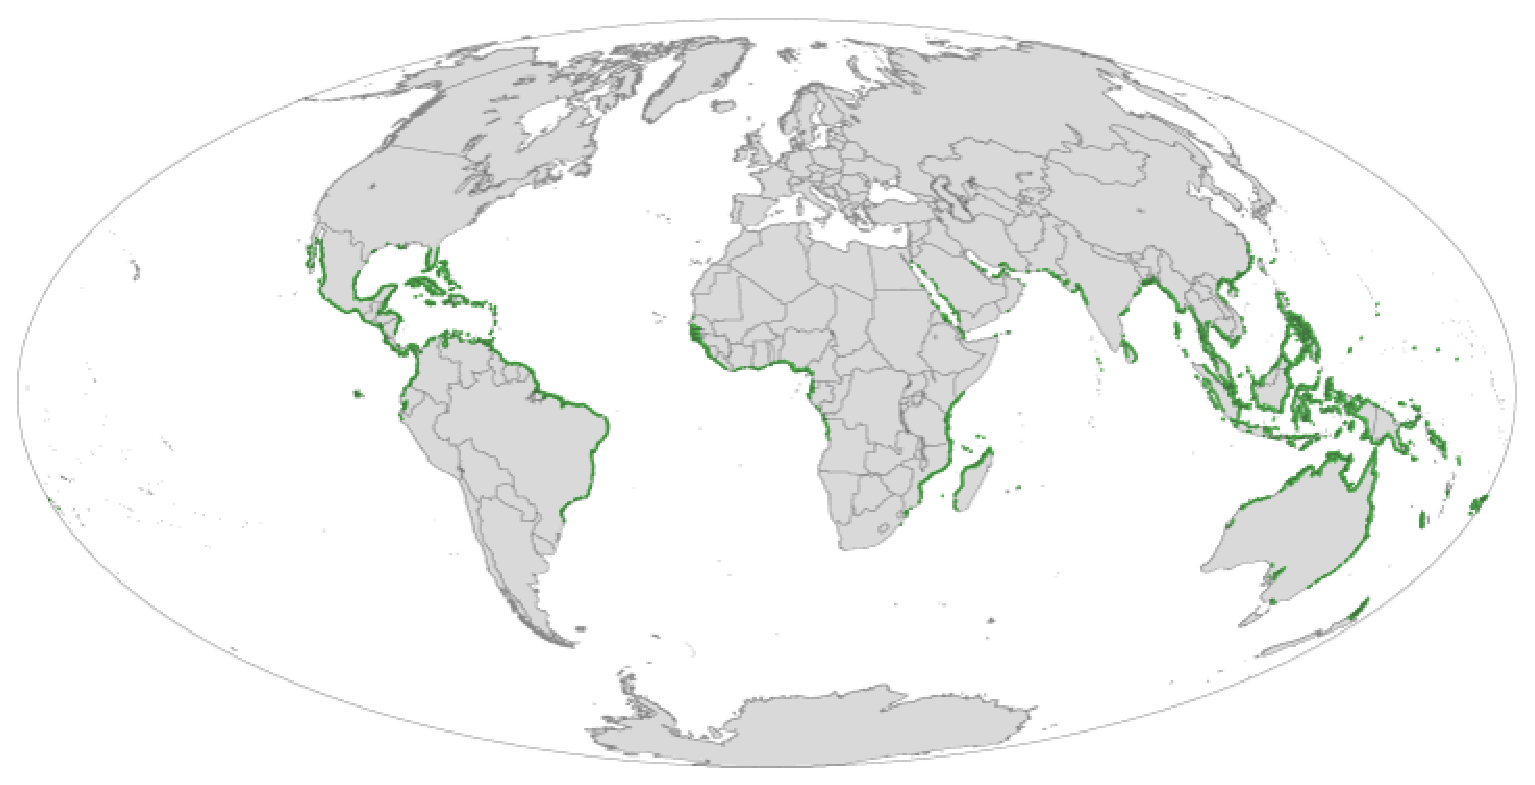
\includegraphics[width=0.8\linewidth]{./Imagenes/distribucion_mundial_mangle.eps}
	\captionsetup{font={footnotesize,it}}
	\caption[Distribución mundial de manglar]{Distribución mundial del manglar. Fuente: Wikimedia Commons.}
	\label{fig:mundial}
\end{figure}

El manglar es un ecosistema delicado y dependiente de los procesos que ocurren fuera de sus fronteras, como pueden ser cambios en las escorrentías de los ríos que afectan a estas zonas, alteraciones en la calidad del agua, provocadas por ejemplo por contaminantes arrastrados por la deriva, o porcentaje de salinidad de las aguas. Esto convierte a mareas, ríos y corrientes litorales como principales agentes alteradores del ecosistema manglar, pero también existe una componente humana importante que afecta directamente.\Sep

Los bosques de mangle de esta región están compuestos por bosque de mangle alto y bosque de mangle bajo. El bosque alto es el situado sobre la línea de costa y su altura varía entre los 5 y los 10 metros, mientras que el bosque bajo se sitúa contiguo al alto en zonas más cercanas a tierra. En el bosque de mangle alto conviven las especies \textit{Rhizophora mangle} y \textit{Laguncularia racemosa}. En el bosque de mangle bajo conviven mayormente las especies \textit{Avicennia germinans} y \textit{Conocarpus erectus}. Estas especies, excepto la última, serán descritas más adelante en el capítulo de Materiales y Métodos (\ref{cap:materialymetodos}).\Sep

En cambio, el manglar es un ecosistema gravemente amenazado. Como se mencionaba, el impacto ambiental, directo e indirecto, no solo procede de la creación de infraestructuras, expansión urbana y desarrollo de industria petrolera sino también de la reconversión en zonas de cría de camarón (figura \ref{fig:camaroneras}) o agricultura costera y salinas (figura \ref{fig:salinas}) que deterioran la calidad del agua. Otras causas del deterioro a escala global de los manglares serían la escasa legislación de la propiedad de recursos naturales, los cambios de actividad de las comunidades costeras, las malas decisiones políticas, la ausencia de planes de desarrollo costero, la depreciación del valor ecológico, la explotación no sostenible o el desconocimiento de las consecuencias \citep{yanez1994}.\Sep

\begin{figure}
	\centering
	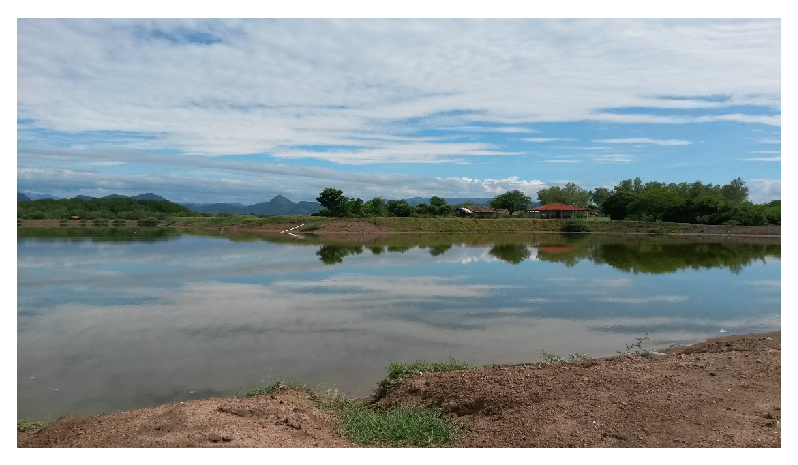
\includegraphics[width=0.9\linewidth]{./Imagenes/Camaronera2.eps}
	\captionsetup{font={footnotesize,it}}
	\caption[Estanques de cría de camarón]{Estanques dedicados a la cría de camarón en el Golfo de Fonseca. Fotografía de Rafael Corrales Andino.}
	\label{fig:camaroneras}
\end{figure}

Una de las posibles soluciones que mitiguen estas causas es la de conocer mejor este ecosistema y su funcionamiento. Precisamente esta es una de las finalidades de este \ac{TFG}.\Sep

El empleo de sensores remotos para proyectos relacionados con el medioambiete y el entorno forestal es una realidad y se han utilizado mucho estas últimas décadas con unos buenos resultados. Como por ejemplo, \cite{bodart2011pre} y \cite{cajacuri2011medicion} realizan un estudio multitemporal de los cambios sufridos por las coverturas forestales, mientras que el estudio de \cite{chen2013multi} se centra precisamente en analizar los cambios en el bosque de mangle hondureño apoyándose en imágenes Landsat. \cite{lee2009applying} destacan la utilización de sensores remotos por la velocidad y precisión a la hora de recabar datos y comparan la utilización de diferentes sensores.\Sep

\begin{figure}
	\centering
	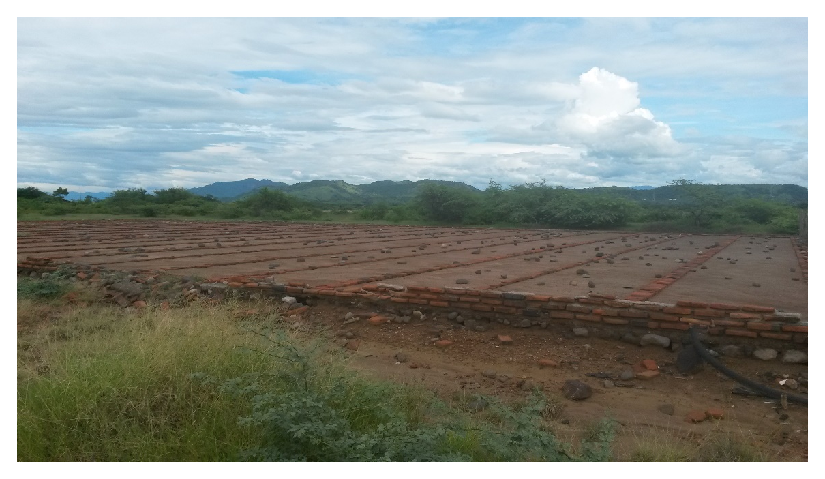
\includegraphics[width=0.9\linewidth]{./Imagenes/Salineras.eps}
	\captionsetup{font={footnotesize,it}}
	\caption[Salineras]{Extensión de terreno dedicada a la producción de sal. Fotografía Rafael Enrique Corrales.}
	\label{fig:salinas}
\end{figure}

\section{Objetivos}
\subsection{Objetivo general}
El objetivo general del trabajo es el de evaluar la posibilidad de emplear imágenes obtenidas con sensores remotos para diferenciar las distintas especies de mangle que se encuentran en el Golfo de Fonseca.\Sep

De todas las especies de mangle existentes en el Golfo de Fonseca se ha decidido tomar tres para este estudio por ser las más predominantes. Son las siguientes:

\begin{itemize}
	\item Mangle Rojo. Nombre científico \textit{Rhizophora mangle} \citep{JimenezRhizophora}.
	\item Mangle Blanco. Nombre científico \textit{Laguncularia racemosa} \citep{JimenezLaguncularia}.
	\item Mangle Prieto. Nombre científico \textit{Avicennia germinans} \citep{JimenezAvicennia}.
\end{itemize}

La hipótesis desde la que se parte es que la respuesta espectral de las diferentes especies de mangle sea lo suficientemente diferente para que este objetivo se cumpla. Esto conduce a la realización de unos objetivos específicos en los que se busca concretar más en el trabajo.

\subsection{Objetivos específicos}
Los objetivos específicos serán el análisis de separabilidad espectral de las especies de mangle del Golfo de Fonseca y determinar la utilidad potencial del empleo de imágenes Landsat para diferenciar las especies analizadas.\Sep

Una vez realizado el análisis de especies se aplicarán los datos extraídos para realizar una clasificación supervisada de una imagen de la zona de estudio captada por el sensor \ac{OLI} y obtenida del servicio de descargas de \ac{USGS}, la denominada \ac{EROS}, gracias a su herramienta Earth Explorer. De esta clasificación se sacarán distintas conclusiones y se analizará la superficie de cada especie de manglar.\Sep

Se parte de la hipótesis de que, dependiendo de los resultados del primer objetivo, sea posible aplicar la experiencia adquirida en el análisis de separabilidad para realizar una clasificación fiable de la zona.\Sep

A esto se le añade el propósito de que, a lo largo de todas las fases del presente trabajo, se estudiará el uso de software libre y las posibilidades que este presenta de cara a futuros proyectos. Estas fases son: redacción del documento, tratamiento, análisis y presentación de los datos así como el tratamiento y procesado de las imágenes. Se presentarán las virtudes y defectos de este tipo de software y se analizarán los problemas presentados.\Sep

Este trabajo tiene como referencia el proyecto de \ac{ISF} en colaboración con la \ac{USC} que tiene como título: ``Investigación y sensibilización sobre la problemática de la actividad acuicola insostenible y promoción de alternativas artesanales basadas en la economía social: puentes entre Golfo de Fonseca y Galicia'' \citep{laborate2014}.

\section{Zona de estudio}\label{sec:zonaestudio}
El área de estudio es el entrante natural del Golfo de Fonseca (figuras \ref{fig:localizacion} y \ref{fig:elevacion}) que abarca la costa pacífica de El Salvador, Honduras y Nicaragua situado entre las latitudes 13,595824ºN – 12,757449ºN y las longitudes 87,994615ºW – 87,115709ºW.\Sep

\begin{figure}
	\centering
	\includegraphics[width=0.8\linewidth]{./Imagenes/localizacion.eps}
	\captionsetup{font={footnotesize,it}}
	\caption[Localización del Golfo de Fonseca]{Localización del Golfo de Fonseca. Fuente: Elaboración propia. Datos: \cite{GADM2012}.}
	\label{fig:localizacion}
\end{figure}

\begin{figure}
	\centering
	\includegraphics[width=0.8\linewidth]{./Imagenes/localizacion_elev.eps}
	\captionsetup{font={footnotesize,it}}
	\caption[Modelo de elevación del Golfo de Fonseca]{Modelo de elevación del Golfo de Fonseca. Fuente: Elaboración propia. Datos: \cite{SRTM2008}}
	\label{fig:elevacion}
\end{figure}

De toda el área forestal de Honduras, que se sitúa en torno a las $54000000000 km^{2}$, los manglares ocupan alrededor de un 1.0\% $515781800 km^{2}$ \citep{anuario2013}. La mayor parte de este porcentaje de manglar se localiza en la costa pacífica del país, en el Golfo de Fonseca, que posee gran riqueza y diversidad de recursos naturales que están amenazados por su sobreexplotación \citep{Jimenez1994}. Esto hace que figure en la lista Ramsar de humedales protegidos a escala mundial \citep{Ramsar2014}. En total cuenta con 409 km de costa abarcando una extensión de $547 km^{2}$.\Sep

El Golfo de Fonseca, caracterizado por tener unas aguas poco profundas, que oscilan entre los 30m y 10m de máxima y 0.5m de mínima, está formado por una serie de ecosistemas interrelacionados formados por estuarios interiores, manglares, costas continentales e insulares. Las cuencas del Río Goascorán y el Río Negro son transfronterizas; la primera es compartida por El Salvador y Honduras y la segunda por Honduras y Nicaragua. Es pues un espacio internacional con humedales compartidos, lo que le otorga una importancia mayor a la hora de ser gestionado.\Sep

Cabe destacar que en 1998 el huracán Mitch devastó una extensa superficie del ecosistema del Golfo de Fonseca causando incontables pérdidas humanas y económicas y cubriendo de lodo las zonas de manglar llegando a provocar un ligero cambio en la línea de costa debido a las crecidas de los ríos y a las amplias mareas \citep{mexico1999honduras}.

\section{Bases teóricas de teledetección} \label{sec:bases}
\subsection{Fundamentos} \label{subsec:fundamentos}
La teledetección es la técnica que nos permite obtener información de los objetos situados en la superficie de la Tierra realizando una observación remota \citep{Curran1991Longman} \citep{chuvieco2002teledeteccion} \citep{schowengerdt2006}. Para que esta observación sea posible debe haber algún tipo de nexo entre el objeto y el sistema sensor u observador. De esta afirmación se extraen los tres elementos básicos de la teledetección: el objeto observado, el sensor y el el flujo energético que los relaciona.\Sep

Hay tres formas de que un sensor pueda adquirir la información del objeto. Estas son: por reflexión, por emisión y por emisión-reflexión.\Sep

\begin{figure}
	\centering
	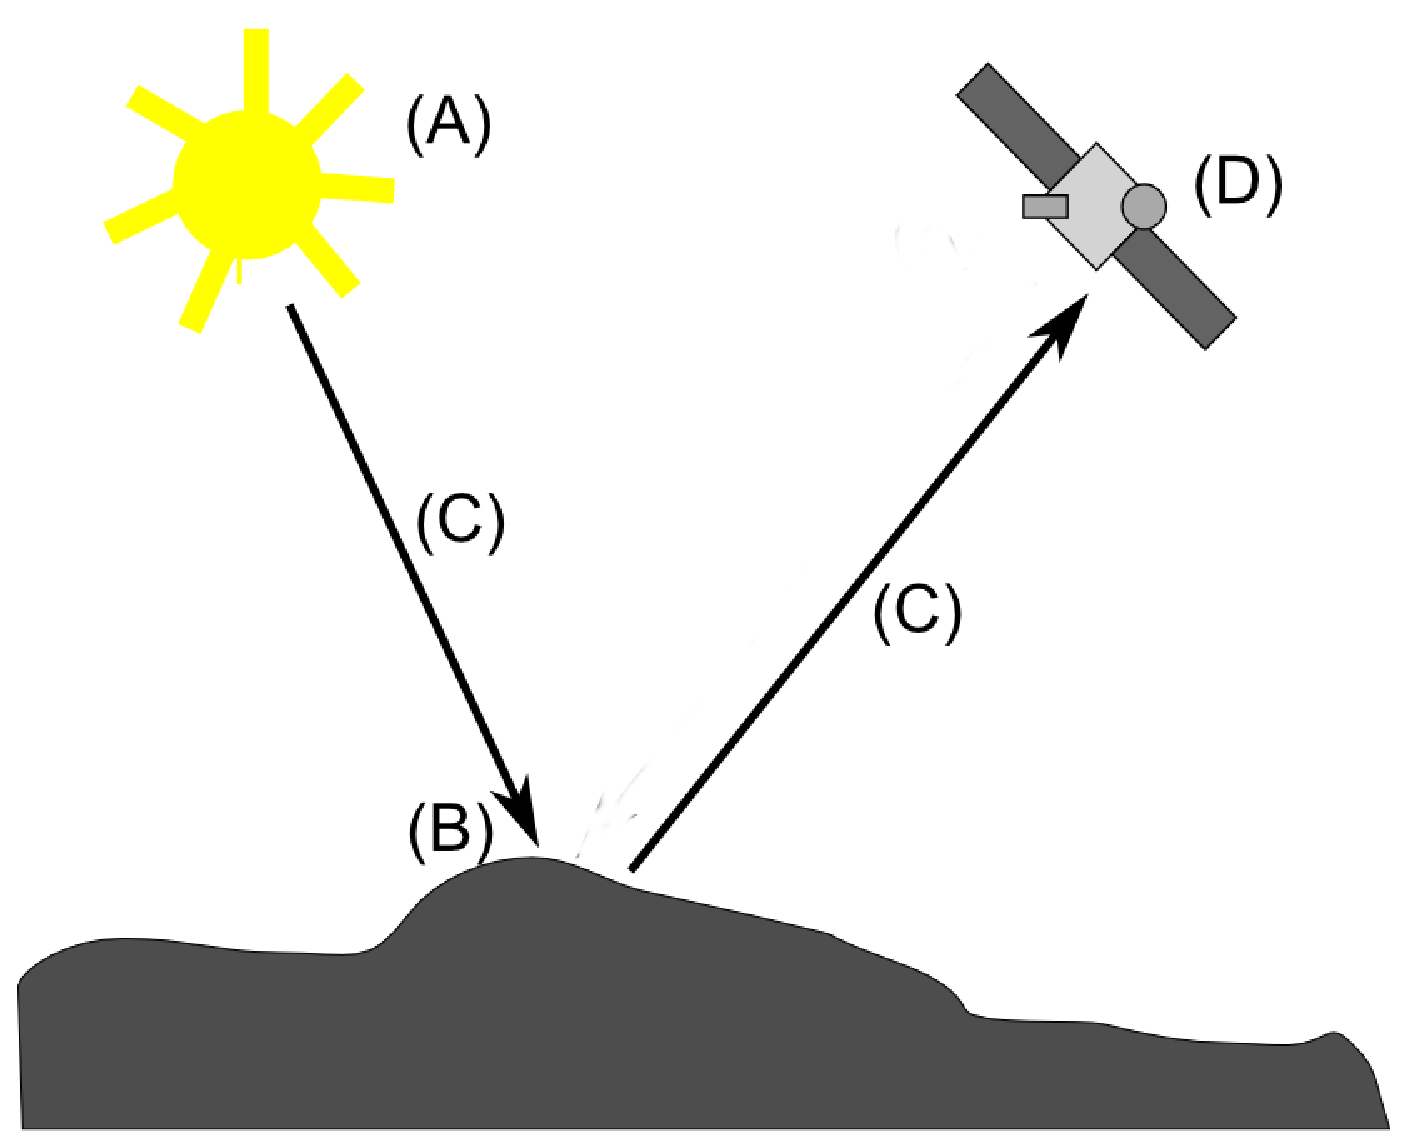
\includegraphics[width=0.4\linewidth]{./Imagenes/Elementos_teledeteccion_modificado.eps}
	\captionsetup{font={footnotesize,it}}
	\caption[Elementos de teledetección]{Elementos de teledetección. Fuente: \cite{Olaya2010}.}
	\label{fig:elementos}
\end{figure}

La primera forma deriva directamente de la reflexión solar (será la empleada en este \ac{TFG}) como se muestra en la figura \ref{fig:elementos}. El Sol (A) ilumina la superficie terrestre que refleja esa energía (C) en función del tipo de cubierta (B). El flujo reflejado es recogido por el sensor (D) que, de ser portado por un satélite, debe atravesar una capa de atmósfera que dispersa y absorbe parte de la señal. El flujo energético entre la cobertura y el sensor constituye una forma de radiación electro-magnética \citep{Olaya2010}.\Sep

\subsection{Espectro Electro-magnético}
Podemos definir cualquier tipo de energía en función de su longitud de onda, de la que se establecen una serie de bandas en donde la radiación electro-magnética manifiesta un comportamiento similar. Esta organización en bandas se denomina espectro electro-magnético (figura \ref{fig:espectro}). Esta comprende desde longitudes de onda corta, como los rayos gamma ($\gamma$) con menos de $10^{-11} m$, a longitudes de onda mayores de un metro como las ondas de radio.\Sep

\begin{figure}
	\centering	
	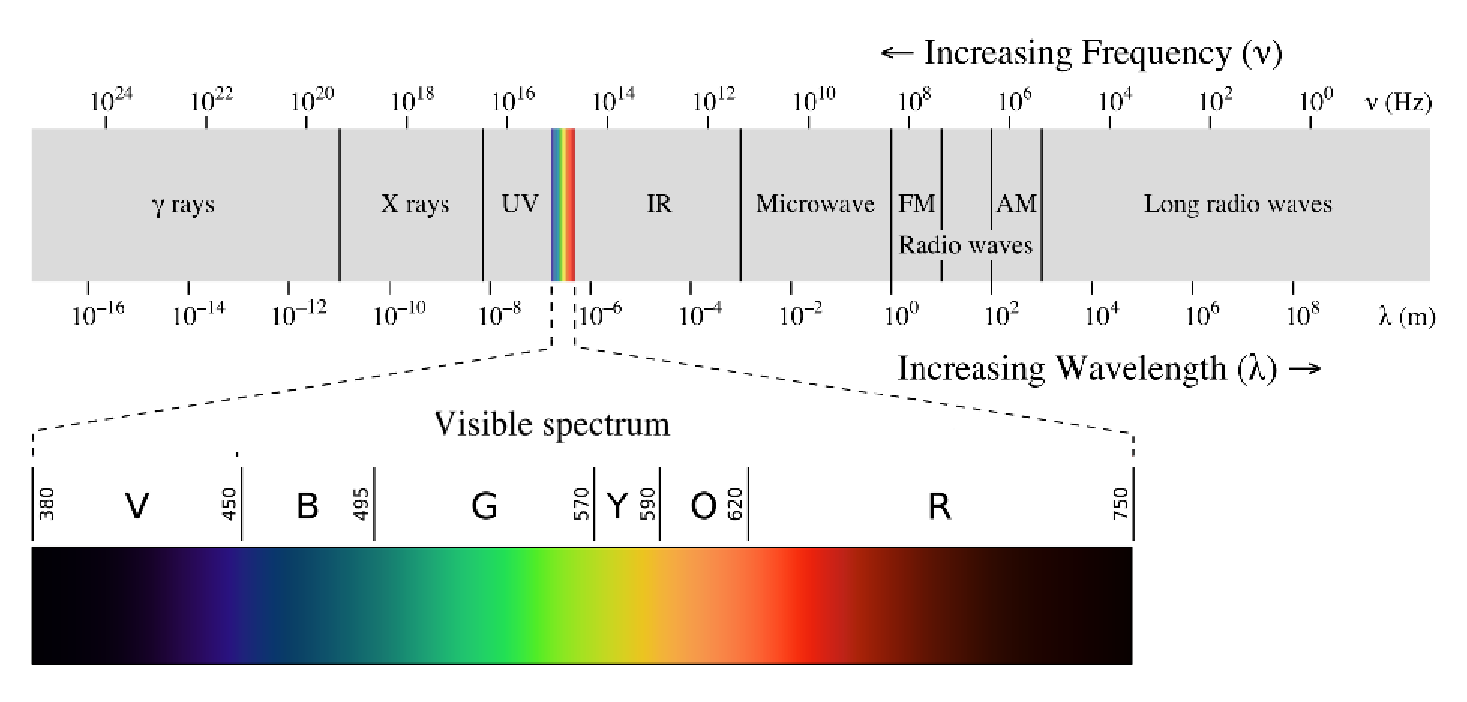
\includegraphics[width=0.9\linewidth]{./Imagenes/Espectro.eps}
	\captionsetup{font={footnotesize,it}}
	\caption[Espectro electro-magnético]{Espectro electro-magnético. Fuente: Wikimedia Commons.}
	\label{fig:espectro}
\end{figure}

En el cuadro \ref{tab:bandas} se destacan la serie bandas espectrales más empleadas en teledetección, siendo su denominación y ancho de banda el generalizado.\Sep

\begin{table}\centering
	\caption[Bandas espectrales utilizadas en teledetección]{Bandas espectrales utilizadas en teledetección.}
	\begin{tabular}{@{}llc@{}}
		\toprule[0.4mm]
		\multicolumn{2}{c}{\textbf{Banda}} & \textbf{L. de onda} \\
		\midrule
		\multirow{3}{*}{Visible} & Azul & $0.4-0.5{\mu}m$ \\
		& Verde & $0.5-0.6{\mu}m$ \\
		& Rojo & $0.6-0.7{\mu}m$ \\
		\midrule
		\multirow{3}{*}{Infrarrojo} & Cercano (IRC) & $0.7-1.2{\mu}m$ \\
		& Medio (IRM) & $1.2-8.0{\mu}m$ \\
		& Térmico (IRT) & $8.0-14.0{\mu}m$ \\
		\midrule
		\multicolumn{2}{c}{Microondas (M)} & $>1mm$\\
		\bottomrule[0.4mm]
	\end{tabular}
	\label{tab:bandas}
\end{table}

El espectro visible es la única radiación electromagnética perceptible por la vista. Como se muestra en el cuadro \ref{tab:bandas} esta banda se divide en otras tres elementales: azul, verde y rojo; en razón de los colores primarios que los ojos perciben a esas longitudes de onda.\Sep

En el caso de la banda infrarroja esta también se divide en tres bandas elementales: \ac{IRC}, \ac{IRM} e \ac{IRT}. El \ac{IRC}, también denominado próximo, es de especial importancia puesto que es utilizado para detectar masas vegetales y concentraciones de humedad. En el \ac{IRM} tenemos que diferenciar el \ac{SWIR} o infrarrojo de onda corta (situado entre 1.2 y 2.5$\mu$m resultando una banda indicada para estimar el contenido en humedad de la vegetación y los suelos) y el \ac{IRM} propiamente dicho (situado entre 2.5 y 8$\mu$m siendo determinante para la detección de focos de alta temperatura como incendios).\Sep

El \ac{IRT} es el indicado para dimensionar las emisiones de temperatura de las cubiertas sobre la superficie terrestre. Es poco utilizado para otros fines.\Sep

Las microondas tienen interés por ser un tipo de energía capaz de penetrar la cubierta nubosa pero no se tendrá en cuenta en este tipo de trabajos.\Sep

En capítulos sucesivos veremos que los valores de los intervalos de longitudes de onda de las bandas tomadas por los sensores satelitales son ligeramente diferentes a los mostrados en este capítulo.

\subsection{Términos y Unidades}
Como se indicó anteriormente, para que se pueda producir la observación remota es preciso que el sensor detecte un flujo energético proveniente de las cubiertas sobre la superficie terrestre. Este flujo energético tiene una intensidad determinada que proviene o está dirigida a una cubierta determinada con una dirección concreta. Se definen a continuación las magnitudes absolutas empleadas en teledetección.

\begin{itemize}
	\item Energía radiante (Q). Indica el total de energía radiada en todas las direcciones. Es medida en Julios (J).
	\item Flujo radiante ($\phi$). Es el total de energía radiada en todas las direcciones por unidad de tiempo. Es medida en vatios (W). Se compone de flujo reflejado ($\phi_{r}$), flujo absorbido ($\phi_{a}$) y flujo transmitido ($\phi_{t}$).
	\item Emitancia radiante (M). Es el total de energía radiada en todas las direcciones por superficie y por unidad de tiempo. Es medida en vatios por metro cuadrado ($Wm^{-2}$).
	\item Irradiancia (E). Es el total de energía radiada sobre una unidad de superficie y por unidad de tiempo. Es equivalente a la emitancia, excepto a que se refiere a la energía incidente y no a la emitida. Es medida en $Wm^{-2}$.
	\item Intensidad radiante (I). Es el total de energía radiada por unidad de tiempo y por ángulo sólido ($\Omega$). Este ángulo es tridimensional y refiere a la sección completa de la energía transmitida (es medido en estéreo-radianes. La intensidad radiante se mide en vatios por estéreo-radian ($Wsr^{-1}$).
	\item Radiancia (L). Es el total de energía radiada en una determinada dirección por unidad de superficie y por ángulo sólido de medida. Es uno de los términos más importantes en teledetección porque es la magnitud que mide el sensor. Se cuantifica en vatio por metro cuadrado y estéreo-radián ($Wm^{-2}sr^{-1}$).
	\item Radiancia espectral ($L_{\lambda}$). Indica el total de energía radiada en una determinada longitud de onda por unidad de área y por ángulo sólido de medida.
\end{itemize}

De igual forma se definen magnitudes relativas que son adimensionales:

\begin{itemize}
	\item Emisividad ($\epsilon$). Es la relación entre la emitancia de la superficie (M) y la emitancia de un emisor perfecto (cuerpo negro) a igual temperatura.
	\item Reflectividad ($\rho$). Es la relación entre el flujo reflejado y el incidente.
	\item Absortividad ($\alpha$). Es la relación entre el flujo absorbido y el incidente.
	\item Transmisividad ($\tau$). Relación entre el flujo transmitido y el incidente.
\end{itemize}

Debido a que la radiancia que capta un sensor depende de la que refleja la cubierta en la que incide, para detectar una cubierta por teledetección se precisa explicar como interactúa con la radiación solar incidente. El flujo incidente ($\phi_{i}$), como ya se mencionó, se descompone en tres términos: flujo reflejado ($\phi_{r}$), flujo absorbido ($\phi_{a}$) y flujo transmitido ($\phi_{t}$), es decir:
\begin{equation}
	\phi_{i}=\phi_{r}+\phi_{a}+\phi_{t}
	\label{eq:flujoinc}
\end{equation}
que expresado en términos relativos:
\begin{equation}
	\frac{\phi_{i}}{\phi_{i}}=\frac{\phi_{r}}{\phi_{i}}+\frac{\phi_{a}}{\phi_{i}}+\frac{\phi_{t}}{\phi_{i}}
	\label{eq:flujorel}
\end{equation}
lo que es igual a la suma de la reflectividad, absortividad y transmisividad ha de ser igual a uno:
\begin{equation}
	1=\rho+\alpha+\tau
	\label{eq:flujo}
\end{equation}
que variando según la longitud de onda ($\lambda$) bastaría con expresarlo de la siguiente manera:
\begin{equation}
	1=\rho_{\lambda}+\alpha_{\lambda}+\tau_{\lambda}
	\label{eq:flujolong}
\end{equation}

La cantidad de flujo incidente que es reflejado, transmitido y absorbido dependen directamente de las características de la cubierta que se está observando y de la longitud de onda a la que se observa. Para conocer fielmente las características de una cubierta conviene observarla a distintas longitudes de onda, lo que permitirá diferenciarla de otras cubiertas susceptibles de ser espectralmente similares.\Sep

La variación de longitud de onda, por ejemplo en el espectro visible, se detecta fácilmente pues se ve afectado en nada menos que el color en el que observamos. Un objeto será rojo, verde o azul si refleja la energía de la banda del espectro correspondiente o si absorbe más intensamente la de las otras bandas.\Sep

El flujo de energía recibida por el sensor depende, además de la reflectividad de la cubierta, de las condiciones atmosféricas, el emplazamiento ambiental de la cubierta y la geometría de la observación. El sensor puede registrar distintos valores para el mismo tipo de cubierta dependiendo de la variación en las condiciones de observación o iluminación. Hay que tener en cuenta que una cubierta vegetal presenta distintos estados biológicos a lo largo del año, lo que añade una componente temporal a la toma de datos. En resumen, los factores que afectan a las características espectrales de una cubierta son:
\begin{itemize}
	\item Ángulos de iluminación y observación, que varían con la latitud, fecha del año y hora de la observación y la posición del sensor.
	\item Modificaciones que el relieve introduce en el ángulo de iluminación, como pueden ser la orientación de las laderas de una montaña o pendientes.
	\item Influencia de la atmósfera, absorción por nubes y dispersión selectiva en distintas longitudes de onda.
	\item Variaciones medioambientales en la cubierta: asociación con otras superficies, homogeneidad que presenta o estado fenológico entre otras.
	\item Sustrato edafológico o litológico, especialmente influyente cuando la cubierta observada presenta una densidad media.
\end{itemize}

\subsection{Firmas espectrales}
Las firmas o signaturas espectrales (figuras \ref{fig:firma} y \ref{fig:biblioteca_esp}), extraído del inglés \textit{spectral signatures}, es la forma de reflejarse que tiene una cubierta a lo largo de distintas longitudes de onda y se utiliza para discriminar una cubierta de otra a partir de una observación remota. Son fundamentales para reconocer cubiertas de interés o extraer parámetros o características intrínsecas a dicha cubierta. La firma espectral se puede obtener de las siguientes fuentes:

\begin{itemize}
	\item Medidas con un radiómetro.
	\item Bibliotecas espectrales.
	\item Simulaciones mediante modelos físicos.
	\item Imagen con la debida resolución espectral.
\end{itemize}

El medio más sencillo de disponer de firmas espectrales son las bibliotecas espectrales. Las bibliotecas espectrales son colecciones de firmas espectrales, tomadas en condiciones controladas por radiómetros en laboratorio, que sirven de referencia para conocer el comportamiento de una cubierta determinada \citep{andinofase1}.

\begin{figure}
	\centering	
	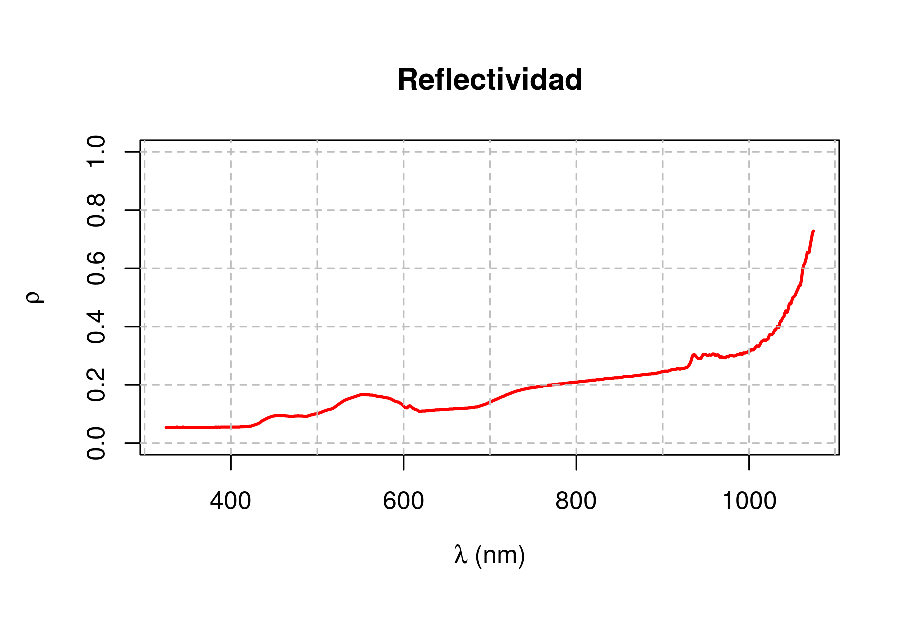
\includegraphics[width=0.7\linewidth]{./Imagenes/Firma_espectral.eps}
	\captionsetup{font={footnotesize,it}}
	\caption[Firma espectral ejemplo]{Firma espectral ejemplo de una cubierta no identificada. Fuente: Elaboración propia.}
	\label{fig:firma}
\end{figure}

Hay numerosos ejemplos de bibliotecas espectrales en Internet, como las del \ac{SIGFIRM} venezolano que recoge el comportamiento espectral de los cultivos en regiones agrícolas de Venezuela \ref{fig:biblioteca_esp}; o la ASTER spectral library de la NASA, que recoge datos de otras tres bibliotecas espectrales: las del \ac{JHU}, \ac{JPL} y \ac{USGS} registrando más de 2400 firmas de materiales como minerales, rocas, suelos y algunas cubiertas artificiales como lo son cemento, aluminio o papel.\Sep

\begin{figure}
	\centering
	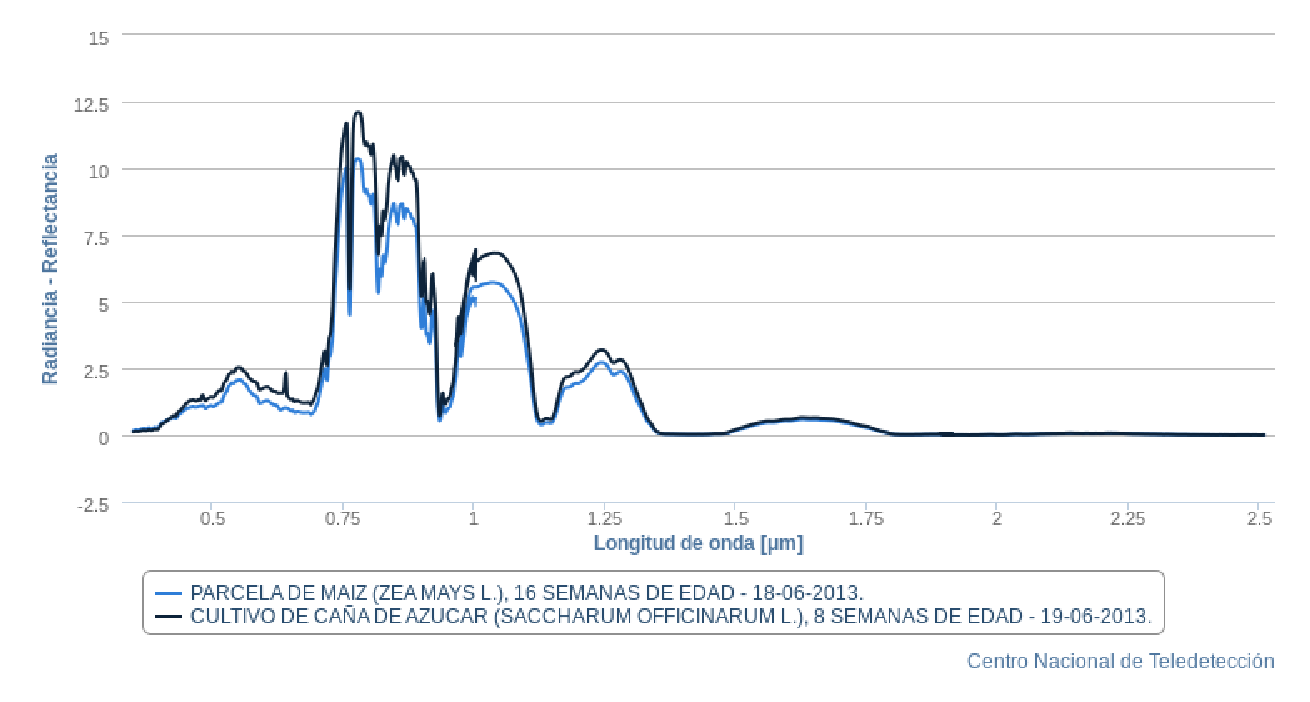
\includegraphics[width=0.7\linewidth]{./Imagenes/biblioteca_espectral_SIGFIRM.eps}
	\captionsetup{font={footnotesize,it}}
	\caption[Biblioteca espectral SIGFIRM]{Biblioteca espectral de maíz y caña de azucar. Fuente: \ac{SIGFIRM}}
	\label{fig:biblioteca_esp}
\end{figure}

\subsection{Sensores}
\label{subsec:sensores}
En el apartado de fundamentos (\ref{subsec:fundamentos}) de este mismo capítulo se indicaba que el sistema sensor era una de los tres componentes principales de la teledetección.\Sep

La clasificación más común de los sensores es según la forma de recibir la energía de las cubiertas, dando lugar a:
\begin{itemize}
	\item Pasivos, donde el sensor recibe la energía emitida por un agente exterior (e.g. el Sol).
	\item Activos, donde el sensor recibe un haz de energía emitido por él mismo (e.g. radares).
\end{itemize}

\subsubsection{Sensores pasivos} \label{subsubsec:sensorespasivos}
En una clasificación más detallada de los sensores pasivos estos se dividen en sensores fotográficos (cámaras analógicas), óptico-electrónicos (exploradores de barrido, de empuje y cámaras de vídeo) y de antena (radiómetros de microondas), en función del procedimiento que emplean para recibir la radiación procedente de los objetos.\Sep

Lo que concierne a este \ac{TFG} serán los sensores pasivos óptico-electrónicos ya que las cámaras analógicas eran más utilizadas en fotogrametría aérea y los radiómetros de microondas trabajan en frecuencias muy elevadas.\Sep

Los sensores óptico-electrónicos combinan una óptica similar a las cámaras analógicas con un sistema de detección electrónica permitiendo prescindir de un soporte sólido de grabación de imágenes. El sensor convierte la señal de radiancia proveniente del objeto en un valor digital. Los sensores exploradores de barrido, que son los más habituales, utilizan un espejo que oscila perpendicularmente a la dirección de la trayectoria.\Sep

Un ejemplo de sensor remoto pasivo de barrido es el \ac{ETM+} montado sobre el satélite Landsat 7. Otro ejemplo de explorador de barrido son los sensores \ac{TM} del Landsat 5, el \ac{OLI} del Landsat 8 (de cuyas imágenes se hará uso en este \ac{TFG} y se le dedicará un parágrafo) o el \ac{AVHRR} del NOAA. De los tres primeros se extraen los cuadros \ref{tab:sensoresTM}, \ref{tab:sensoresETM} y \ref{tab:sensoresOLI}.\Sep

\begin{table}
	\centering
	\caption[Bandas en el sensor TM]{Bandas en el sensor TM del proyecto Landsat. Fuente: USGS.}
	\begin{tabular}{@{}cccc@{}}
		\toprule[0.4mm]
		Banda & Nombre & L. onda ($\mu$m) & Resolución (m)\\
		\midrule
		1 & B & 0.45--0.52 & 30 \\
		2 & G & 0.52--0.60 & 30 \\
		3 & R & 0.63--0.69 & 30 \\
		4 & NIR & 0.76--0.90 & 30 \\
		5 & NIR & 1.55--1.75 & 30 \\
		6 & TIR & 10.40--12.50 & 120 \\
		7 & MIR & 2.08--2.35 & 30 \\
		\bottomrule[0.4mm]
	\end{tabular}
	\label{tab:sensoresTM}
\end{table}

\begin{table}
	\centering
	\caption[Bandas en el sensor ETM+]{Bandas en el sensor ETM+ del proyecto Landsat. Fuente: USGS.}
	\begin{tabular}{@{}cccc@{}}
		\toprule[0.4mm]
		Banda & Nombre & L. onda ($\mu$m) & Resolución (m)\\
		\midrule
		1 & B & 0.45--0.52 & 30 \\
		2 & G & 0.52--0.60 & 30 \\
		3 & R & 0.63--0.69 & 30 \\
		4 & NIR & 0.77--0.90 & 30 \\
		5 & NIR & 1.55--1.75 & 30 \\
		6 & TIR & 10.40--12.50 & 60 \\
		7 & MIR & 2.08--2.35 & 30 \\
		\bottomrule[0.4mm]
	\end{tabular}
	\label{tab:sensoresETM}
\end{table}

\begin{table}
	\centering
	\caption[Bandas en el sensor OLI]{Bandas en el sensor OLI del proyecto Landsat 8. Fuente: USGS.}
	\begin{tabular}{@{}cccc@{}}
		\toprule[0.4mm]
		Banda & Nombre & L. onda ($\mu$m) & Resolución (m)\\
		\midrule
		1 & Coastal & 0.43--0.45 & 30 \\
		2 & B & 0.45--0.51 & 30 \\
		3 & G & 0.53--0.59 & 30 \\
		4 & R & 0.64--0.67 & 30 \\
		5 & NIR & 0.85--0.88 & 30 \\
		6 & SWIR & 1.57--1.65 & 30 \\
		7 & SWIR & 2.11--2.29 & 30 \\
		9 & Cirrus & 1.36--1.38 & 30 \\
		\bottomrule[0.4mm]
	\end{tabular}
	\label{tab:sensoresOLI}
\end{table}

Otro tipo de sensor pasivo son los exploradores de empuje. En estos se elimina el espejo oscilante, en cuyo lugar se disponen una serie de detectores que cubren todo el campo de visión del sensor que exploran, en cada momento, una línea completa desplazándose esta línea simultáneamente con la plataforma. Estos exploradores permiten aumentar la resolución espacial y agilizan la detección de datos al hacer la conversión radiancia a valor digital por línea y no por píxel como los anteriores.\Sep

Ejemplos de exploradores de empuje son los sensores \ac{HRV} del SPOT o los senores portados por los satélites IKONOS o Quickbird.

\subsection{Resoluciones}

Se define la resolución del sistema sensor en teledetección como la capacidad para discriminar información de detalle en un objeto. Otra definición utilizada es la de valor mínimo determinado para alguna de las variables que definen a una imagen digital \citep{chuvieco2002teledeteccion} .\Sep

El concepto de información de detalle de la primera definición comprende tanto al detalle espacial que ofrece el sensor como a número y anchura de bandas espectrales, a su carencia temporal y a la capacidad para distinguir variaciones en la energía que detecta. Esto significa que el concepto de resolución se basa en el conjunto de:
\begin{enumerate}
	\item Resolución espacial.
	\item Resolución espectral.
	\item Resolución radiométrica.
	\item Resolución temporal.
\end{enumerate}

\subsubsection{Resolución espacial}
Designa el objeto más pequeño que es posible distinguir en la imagen digital. Se mide en milímetros sobre la imagen o metros sobre el terreno y depende de la longitud focal del sensor y altura sobre la superficie. En sensores óptico-electrónicos se utiliza el \ac{IFOV}, que se define como la sección angular que observa el sensor en un momento determinado.
\begin{equation}
	d=2h\tan(IFOV/2)
	\label{eq:res_esp}
\end{equation}
donde $d$ es la distancia sobre el terreno que abarca con ese ángulo \ac{IFOV}, y $h$ la altura del sensor sobre el terreno. Esta mínima unidad de información en la imagen es la que se denomina píxel.\Sep

La resolución espacial de un sensor, como ya se ha mencionado, depende de varios factores, como la altura orbital, la longitud focal y el número de detectores. En los sensores de antena, la resolución espacial depende del tamaño de la antena, la altura de la plataforma y el ángulo de incidencia.\Sep

Dependiendo de la resolución espacial tenemos cuatro tipos de sensores:
\begin{enumerate}
	\item De alta resolución. Con resoluciones próximas al metro de ancho.
	\item De recursos naturales. Con resoluciones entre los 25 x 25m y 1000 x 1000m.
	\item De baja resolución. Por lo general montados sobre satélites geoestacionarios y dedicados a ámbitos metorológicos, cuentan con una resolución espacial que puede llegar a los 5 x 5km.
\end{enumerate}

\subsubsection{Resolución espectral}
Designa el número y anchura de bandas espectrales que puede discriminar el sensor. Es muy importante la capacidad del sensor para registrar simultaneamente el comportamiento de un mismo objeto en varias bandas del espectro. En definitiva, un sensor tendrá mayor resolución cuanto mayor número de bandas detecte, facilitando así la caracterización espectral de las cubiertas.\Sep

Es evidente la importancia que tiene la elección del sensor en cuanto al número de bandas, ancho y longitud de las mismas dependiendo del objetivo del trabajo a realizar. Por ejemplo, para la detección de vegetación se hace más importante disponer de bandas del \ac{IRC} e \ac{IRM} más que del \ac{IRT}, en cambio para detectar incendios sí es importante disponer de la banda del \ac{IRT}.

\subsubsection{Resolución radiométrica}
Designa la sensibilidad del sensor o su capacidad para detectar las variaciones en la radiancia espectral. En los equipos digitales, como por ejemplo el sensor \ac{ETM+}, la imagen es codificada en un formato binario, por lo que la resolución radiométrica se identifica con el rango posible de valores que almacena el sensor, medido como el número de bits que necesita cada valor numérico para almacenarse. El mencionado \ac{ETM+} ofrece una resolución de 8 bits, es decir, 256 niveles por píxel.\Sep

La importancia de este tipo de resolución se hace patente a la hora de interpretar las imágenes, sobre todo cuando esta interpretación es digital, ya que el ordenador aprovecha todo el rango de resolución radiométrica.

\subsubsection{Resolución temporal}
Designa la frecuencia de cobertura que proporciona el sensor, es decir, la periodicidad con la que adquiere imágenes de la misma zona de la superficie terrestre. Esto depende de las características orbitales de la plataforma (altura, velocidad e inclinación) y del diseño del sensor (del ángulo total de apertura). La resolución temporal dependerá también de las condiciones atmosféricas puesto que una amplia cobertura nubosa impedirá la observación y dilatará dicha temporalidad.\Sep

Las variaciones en la resolución temporal responden al objetivo para el que esté diseñado el sensor, pudiendo llegar a los 15 o 30 minutos de los satélites meteorológicos como Meteosat y hasta los 15 o 31 días de los satélites de recursos naturales como el Landsat o Spot.

\subsubsection{Resolución angular}
Designa la capacidad de un sensor de tomar instantáneas de una misma porción de terreno desde distintas órbitas. Esto se relaciona con la resolución temporal en que, tomando el supuesto de que en un momento dado la cobertura nubosa impide la observación, el sensor tome la imagen desde una órbita cercana en otro lapso de tiempo inclinándose para poder hacerla. Esta capacidad reduce el efecto de reflectividad bidireccional que presentan algunas cubiertas y los efectos de absorción y dispersión de la atmósfera.\Sep

En el cuadro \ref{tab:resoluciones} se comparan las diferentes resoluciones de los principales sensores para fines medioambientales que hay actualmente en órbita.

\begin{table}[ht]
	\centering
	\caption[Resoluciones de varios sensores]{Resoluciones de varios sensores.}
	\begin{tabular}{@{}ccccc@{}}
	\toprule[0.4mm]
	& Landsat 8 & QuickBird & Spot 6 & IKONOS \\
	& OLI & & HRV & \\
	\midrule
	R. Espacial MS (m) & 30--60 & 2.44--2.88 & 6 & 3.2--4 \\
	R. Espectral (nm) & 450--12500 & 450--900 & 455--890 & 445--853 \\
	R. Radiométrica (bits) & 8 & 11 & 12 & 11 \\
	R. Temporal (días) & 16 & 1--3 & 1--3 & 3 \\
	\bottomrule[0.4mm]
	\end{tabular}
	\label{tab:resoluciones}
\end{table}

\subsection{Correcciones}
Como se exponía anteriormente la imagen digital tomada por el sistema sensor se compone de una malla de píxeles que toman un valor numérico concreto obtenido a partir de la radiancia observada. Ese valor numérico que codifica cada píxel es el llamado \ac{ND}. La propiedad más ventajosa de esos \ac{ND} es que pueden traducirse a color o niveles de gris, por ejemplo mediante el uso de un monitor, dependiendo, la intensidad, del \ac{ND}. A partir del \ac{ND} visualizado se pueden hacer operaciones de realce que no modificarán su valor pero sí harán que se vea con diferente intensidad. A este nuevo valor se le llamará \ac{NV}. El \ac{ND}, en cambio, es utilizado para operaciones de interpretación digital, especialmente cuando estas se relacionan con parámetros como la reflectividad o la temperatura.\Sep

La mejor forma de ver una imagen es como si fuera un sistema de tres dimensiones, donde las dos primeras dimensiones corresponden a la posición geográfica de la imagen y la tercera corresponde al \ac{ND}.\Sep

Las correcciones propiamente dichas son aquellos procesos con los que se eliminan anomalías detectadas en la imagen, tanto de localización como en la radiometría de los píxeles. La finalidad de estos procesos es la de disponer los datos de la forma más cercana a lo que sería una adquisición idónea (e.g. posición geográfica correcta). Es posible que la corrección más importante sea la geográfica, pues aporta validez cartográfica a los resultados y permite la conexión con otros datos geográficos en un \ac{SIG}.\Sep

Las principales fuentes de error que provocan la necesidad de realizar correcciones son:
\begin{itemize}
	\item Distorsiones originadas por la plataforma. El alabeo, el cabeceo o el giro lateral son movimientos que modifican la altitud de órbita del satélite, la velocidad o la orientación, lo que se traduce en problemas en la adquisición de las imágenes. Problemas como lo son cambios en la escala de adquisición o distorsiones en la geometría.
	\item Distorsiones provocadas por la rotación terrestre. En algunos sensores la toma de la imagen supera los 20 segundos, tiempo en el que la Tierra se desplaza en rotación unos 6 kilómetros.
	\item Distorsiones provocadas por el sensor. Distorsiones debidas al tipo de sensor relacionadas con el ángulo de barrido o el campo de visión global, provocando distorsiones cuanto más alejados están los píxeles del nadir.
	\item Distorsiones provocadas por la atmósfera. Los elementos de la atmósfera causan una modificación en la obtención de la señal original de la superficie terrestre. El efecto más importante es la dispersión, que implica un aumento de la señal recibida por el sensor.
\end{itemize}

La última de la distorsiones, la atmosférica, resulta importante de corregir para generar índices espectrales.\Sep

\subsubsection{Correcciones radiométricas}
Las correcciones radiométricas son aquellas técnicas que modifican los \ac{ND} originales con el objetivo de acercar su valor al que sería obtenido bajo condiciones ideales. Son correcciones radiométricas:
\begin{itemize}
	\item Restauración de líneas o píxeles perdidos. La imagen presenta líneas blancas o negras píxeles de aspecto contrastado al resto. Es una corrección aproximada, puesto que no se pueden poner píxeles de valor correcto donde no hay información.
	\item Corrección del bandeado de la imagen. Es especialmente perceptible en zonas de agua y problemático en los exploradores de empuje. Es un defecto periódico.
	\item Cálculo de reflectividades. Es una corrección muy importante para el análisis e interpretación de imágenes, pues como se decía anteriormente, es preferible trabajar con términos físicos que con \ac{ND}. Particularmente es importante a la hora de comparar datos con otros obtenidos con radiómetros de campo (uno de los objetivos de este \ac{TFG}).
	\item Cálculo de temperaturas.
	\item Detección de nubes.
\end{itemize}

\subsubsection{Correcciones geométricas}
Este tipo de correcciones incluyen los cambios en la posición que los píxeles ocupan en la imagen digital. Son correciones basadas en funciones numéricas que se aplican sobre la geometría de la imagen y la modifican.\Sep

\begin{eqnarray}
	f(c') & = & f_{1}(c,l) ; f(x,y) \\
	f(l') & = & f_{2}(c,l) ; f(x,y)
	\label{eq:correcgeom}
\end{eqnarray}\Sep

Las coordenadas columna y línea $c'$ y $l'$ de la imagen corregida son función de las coordenadas columna y línea de la imagen de entrada $c$ y $l$ o de las coordenadas del mapa al que se pretende superponer la imagen $x$ e $y$. Se trata de encontrar una relación que convierta los \ac{ND} de la imagen a su posición cartográfica en la proyección requerida (en este caso a la \ac{UTM}). Esto permite, entre otras cosas, hacer un mosaico con más imágenes para ampliar la cobertura de la imagen.\Sep

Hay dos procedimientos de corrección geométrica que se pueden aplicar a una imagen que se enumeran a continuación:

\begin{enumerate}
	\item Corrección a partir de modelos orbitales. Corrige los errores provocados por fuentes conocidas a partir de aplicar transformaciones inversas a las que realiza el sensor en el momento de la adquisición de los datos. Se necesita conocer con precisión las características orbitales de la plataforma y las especificaciones del sensor. Se corrigen de esta forma los errores sistemáticos
	\item Corrección a partir de puntos de control. Modela el error geométrico a partir de puntos de control repartidos a lo largo de la zona de la imagen. Estos puntos son de coordenadas conocidas y se asume que sean lo suficientemente representativos de las deformaciones de la imagen.
\end{enumerate}

El primero de los procedimientos es especialmente indicado para aquellas imágenes en las que no se pueden reconocer puntos de control, como imágenes marinas o con una amplia cobertura nubosa o bien sean imágenes con una resolución espacial en la que no se puedan establecer puntos de control con garantías. Por esta última razón es el tipo de corrección geométrica indicada para sensores de muy baja resolución espacial como los de plataforma de órbita geoestacionaria.\Sep

El método de corrección a partir de puntos de control requiere de la intervención humana, lo que resulta tedioso en comparación con el primer método. En cambio ofrece mayor precisión en la corrección dependiendo, evidentemente, de la medida en que en la imagen se puedan detectar los puntos de control establecidos.\Sep

\subsection{Clasificación de imágenes}
La clasificación es el último paso en el análisis de imágenes digitales mediante teledetección (se beneficia de los procesos de correcciones, realces y fusiones de imágenes) y de ella derivan los productos cartográficos finales en forma de mapas temáticos. El \ac{ND} pasa de reflejar el nivel de reflectancia a tener un valor categórico concreto que puede etiquetarse con un tipo concreto de superficie. Se genera así cartografía temática y facilita el trato estadístico de la información.\Sep

Hay numerosos métodos de clasificación que se desgranarán más adelante y que deben cumplir los siguientes requisitos:

\begin{itemize}
	\item Fiabilidad.
	\item Reproducible por otros con las mismas variables de entrada.
	\item Robustez. No debe ser sensible a pequeños cambios en las condiciones de entrada.
	\item Exhaustividad.
	\item Objetividad. No debe estar marcado por las decisiones del intérprete.
\end{itemize}

Uno de los problemas más comunes en la clasificación es la posible similitud entre dos o más cubiertas o inmersión de una sobre otra, que provoca que estas no se definan correctamente. Esto se podría solucionar ampliando la resolución espacial o aplicando la variable temporal a las imágenes (muy apto para discriminar masas vegetales debido a la evolución estacional). También se podría acudir a información auxiliar como topografía del terreno o tipos de suelo.

\subsubsection{Fases de la clasificación}
La clasificación consta de los siguientes puntos que dependiendo del tipo de clasificación, supervisada o no supervisada, se utilizarán de un modo u otro estas fases.
\begin{enumerate}
	\item Fase de entrenamiento.
Para la interpretación de la imagen es necesaria una experiencia previa que permita identificar las categorías según su textura, tono, tamaño o situación de los píxeles que la componen.

La finalidad de la fase de entrenamiento es definir un rango de valores de \ac{ND} que en conjunto describan las características de una cubierta concreta. A esto se le llama área de entrenamiento. Una cubierta no se define únicamente por un valor de \ac{ND} debido a la dispersión en el comportamiento espectral.

Se deberá seleccionar una muestra de píxeles de la imagen que representen lo más fielmente posible a la categoría de interés. A partir de esta muestra se podrán calcular los \ac{ND} medios y la variabilidad de cada categoría de las bandas que intervienen en la clasificación. Por lo tanto, las áreas de entrenamiento deben estar bien identificadas, deben ser suficientemente homogéneas y deben cubrir todas las clases.

En el método supervisado, se seleccionan los píxeles representativos teniendo en cuenta la experiencia en campo o el conocimiento previo del comportamiento espectral de las cubiertas por parte del usuario. Mientras, el método de clasificación no supervisado se basa en la búsqueda autónoma de las muestras dentro de la imagen.

El problema más común en la definición de clases es que el tipo de clase informacional (constituyen la leyenda del trabajo e.g. tipos de suelo) no corresponda con el tipo de clase espectral (ofrecen una respuesta espectral similar). Puede darse el caso de que una cubierta esté representada por varias clases espectrales, que varias cubiertas estén representadas por una sola clase espectral o que varias clases informacionales se correspondan con varias clases espectrales \citep{chuvieco2002teledeteccion}.

	\item Fase de asignación.
En esta fase a cada uno de los píxeles de la imagen se le asigna una clase obteniendo así una nueva imagen con los \ac{ND} expresando una categoría temática diferente. Los criterios de asignación definen un área de dominio, en torno al centro de cada categoría. Por lo tanto, si el \ac{ND} del píxel se encuentra dentro de esa área será asignado a esa clase.

Los clasificadores más habituales son:
\begin{itemize}
	\item Clasificador de mínima distancia: el píxel se asigna a la clase más cercana espectralmente.
	\item Clasificador de paralelepípedos: permite al usuario señalar los umbrales de dispersión espectral asociados a cada clase.
	\item Clasificador de máxima probabilidad (maximun likehood): el píxel se asigna a aquella clase con la que tenga mayor probabilidad de pertenencia.
\end{itemize}
	\item Obtención y presentación de resultados.
	\item Verificación de resultados.
\end{enumerate}

%CAPÍTULO 2. MATERIAL Y MÉTODOS
%MARCOS RIAL DOCAMPO
%Parte del documento principal TFG

%%%%%%%%%%%%%%%%%%%%%%%%
%% MATERIAL Y MÉTODOS %%
%%%%%%%%%%%%%%%%%%%%%%%%


\chapter{Material y métodos}
\label{cap:materialymetodos}

\section{Estudio radiométrico}
En este caso, obtendremos del estudio radiométrico firmas espectrales del tipo monobanda. Estas se caracterizan porque la respuesta de los objetos analizados es contenida en un solo canal continuo de datos \citep{andinofase1}.%\Sep

La meteorología y la difícil accesibilidad de la zona hicieron aconsejable hacer una toma de muestras y realizar la observación en un estudio. El material vegetal utilizado en el estudio fueron muestras recientes de hojas tomadas de árboles de cada especie como se describe en la metodología de obtención de firmas espectrales de \cite{andinofase2} y como se puede apreciar en las figuras \ref{fig:mangle_recolectado} y \ref{fig:curva_espectral}.

\begin{figure}
	\centering
	\includegraphics[width=0.9\linewidth]{./Imagenes/Mangle_recolectado.eps}
	\captionsetup{font={footnotesize,it}}
	\caption[Mangle recolectado]{Hojas de las especies de mangle a analizar. Fotografía de Rafael Corrales.}
	\label{fig:mangle_recolectado}
\end{figure}

\begin{figure}
	\centering
	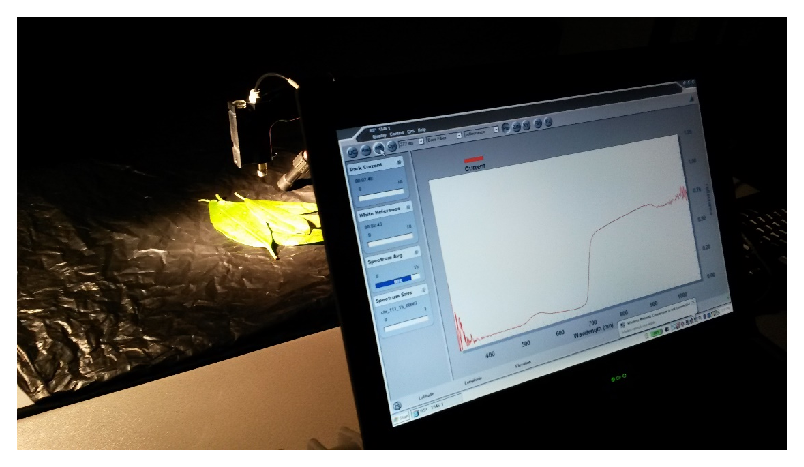
\includegraphics[width=0.9\linewidth]{./Imagenes/Curva_espectral.eps}
	\captionsetup{font={footnotesize,it}}
	\caption[Obtención de firmas]{Momento de la obtención de las firmas espectrales de una especie. Fotografía de Rafael Corrales.}
	\label{fig:curva_espectral}
\end{figure}

\subsection{Datos}\label{subsec:datos}
Los datos obtenidos por el profesor Rafael Enrique Corrales con el espectro-radiómetro de campo se presentan en cuatro archivos de extensión .dat de texto simple, uno para cada especie más uno del conjunto que no se utilizará.%\Sep

La característica principal de estos datos es que abarcan un amplio rango espectral de forma continuada, similar a lo que ocurre en la obtención de una imagen, pero en este caso los datos serían solamente de un punto, no de una superficie extensa. El rango espectral captado por el espectro-radiómetro comprende de 324.5 - 1075,5 nm almacenando la reflectividad media para intervalos de onda de 1nm.%\Sep

Simultáneamente a la toma de datos se visitaron puntos donde era conocida la existencia de mangle (cuadro \ref{tab:puntos}). Estos estrictamente no son puntos de control porque no se trata de puntos en los que no solo existe la cobertura de un tipo de mangle concreto sino que pueden confluir varias cubiertas en el mismo punto. En ellos se observaron la certeza del cambio en la existencia de mangle y alguna de las causas que lo motivan, como la presencia de salineras y estanques de camarón. En algunos casos, como el de La Brea la presencia de R. mangle es para reducir el impacto visual de las camaroneras. En otras zonas como en Los Ganchos, la pérdida de cobertura de mangle es debida a la dinámica de la costa provocada por la desembocadura del río Nacaome.

\begin{table}[ht]
	\centering
	\begin{tabular}{@{}ccll@{}}
	\toprule[0.4mm]
	East & North & Nombre & Epecies existentes\\
	\midrule
	452379 & 1476560 & Pasadero de los Pericos & \textit{R. mangle}.\\
	450493 & 1476503 & Punta de los Elotes & \textit{R. mangle} y \textit{L. racemosa}\\
	448571 & 1484829 & Corinto & \textit{R. mangle} y \textit{L. racemosa}\\
	438047 & 1488915 & Jiote Grande & \textit{R. mangle}, \textit{L. racemosa} y \textit{A. germinans}\\
	434163 & 1487386 & Los Ganchos & \textit{R. mangle}\\
	440251 & 1489561 & La Brea & R. mangle, \textit{L. racemosa} y \textit{A. germinans}\\
	\bottomrule[0.4mm]
	\end{tabular}
	\captionsetup{font={footnotesize,it}}
	\caption[Puntos de control]{Serie de puntos conocidos de existencia de manglar con la especie predominante.}
	\label{tab:puntos}
\end{table}

\section{Software} \label{sec:software}
El uso de software libre en general es un recurso a tener en cuenta para realizar trabajos técnicos que utilizan un componente informático \citep{MatellanOliveira2004} \citep{Mas2005software}. En concreto es uso de este tipo de software en trabajos sobre recursos medioambientales cobra importancia principalmente por, entre otras cosas:

\begin{enumerate}
	\item Abarata el coste del proyecto al ser bajo o nulo el coste de una licencia de uso.
	\item Cuenta con un buen soporte y servicio técnico llevado en algunos casos por comunidades de usuarios y a largo plazo. Se evita la obsolescencia del producto.
	\item Formatos estandarizados que permiten la interoperabilidad.
	\item Se centra en proporcionar un servicio y no un producto.
\end{enumerate}

Este \ac{TFG} se ha hecho íntegramente con software libre distribuido bajo licencia GNU GPL salvo que se indique lo contrario, utilizando los programas seguidamente mencionados sobre un sistema operativo GNU/Linux, en concreto sobre la distribución Ubuntu 14.04\footnote{\url{http://www.ubuntu.com/}}.%\Sep

Adicionalmente se ha hecho un control de versiones remoto con el software Git\footnote{Otra opción en lo que a control de versiones se refiere sería la del software \ac{SVN} \citep{Latex2011} pero este solamente permite hacer un control local de los cambios.} que, mediante repositorios, permite gestionar un historial de ficheros y carpetas recordando y organizando el contenido en cada momento documentando los cambios que ha sufrido y quién y por qué los ha realizado. Permite, por tanto, recuperar el documento a versiones anteriores o revisar el proceso de desarrollo del mismo funcionando como respaldo. De esta forma se permite el acceso a los archivos por la plataforma web GitHub de forma pública\footnote{El código de este trabajo es accesible desde la página web \url{https://github.com/MarcosRial/TFG}}. La interfaz gráfica utilizada ha sido SmartGit\footnote{\url{http://www.syntevo.com/smartgit/}} \citep{GmbH2015} libre y de uso gratuito para fines no comerciales y donde se pueden hacer cómodamente la mayoría de las operaciones de control de cambios.%\Sep

\paragraph{R}
Para el tratamiento de los datos se ha utilizado el software estadístico de uso libre R Project for Statistical Computing, más conocido como R\footnote{\url{http://www.r-project.org/}} \citep{R2013} en su versión 3.2.0. R puede definirse como un software de análisis estadísticos, como un generador de gráficos o como un lenguaje de programación. Si bien es un software pensado para su uso sobre interfaces de código, para la realización de este \ac{TFG} se ha utilizado la interfaz gráfica del software libre RStudio\footnote{\url{https://www.rstudio.com/}}, bajo licencia AGPL, con el fin de hacer que su uso resulte más amigable.%\Sep

R, como la mayoría de software que funciona sobre sistema operativo GNU/Linux, se compone de módulos o paquetes que se incorporan a una base del programa, llamado \textit{R core}, para extender sus posibilidades y funciones. Actualmente el número de paquetes de R existentes ronda los 4000, desarrollados por usuarios y programadores de todo el mundo. Esta cifra se incrementa ya que periódicamente se suben paquetes a la red de repositorios oficial \ac{CRAN}\footnote{\url{http://cran.r-project.org/}}.%\Sep

R es uno de los lenguajes más utilizados en estadística. Adicionalmente abarca otros muchos campos debido a la cantidad de librerías disponibles como tratamiento de imágenes satélite o clasificación supervisada.

\paragraph{GRASS GIS}
Para el tratado de imágenes Landsat y su posterior clasificación se utiliza el programa de \ac{SIG} gratuito y de código abierto \ac{GRASS}\footnote{\url{http://grass.osgeo.org/}} \citep{GRASS_GIS_software}. GRASS es un proyecto de la \ac{OSGeo}. Es un potente software en lo que a utilización de manejo y análisis de información geoespacial se refiere. Su funcionalidad es similar a otros programas \ac{SIG} como QGIS\footnote{\url{http://www.qgis.org/es/site/}}, en los cuales, mediante extensiones aplicadas a la base del programa podemos ampliar sus funciones y adaptarlas a nuestras necesidades \citep{neteler2002open}. Al igual que R, \ac{GRASS} se puede utilizar mediante una interfaz de código pero se optó por la utilización de una interfaz gráfica de usuario (la propia del software) que facilita y agiliza mucho el trabajo.%\Sep

La versión utilizada es la 6.4.3 estable. No obstante durante la realización de este \ac{TFG} se liberaron la versión de desarrollo 6.4.4 y la versión estable 7.0 que fueron utilizadas como alternativa a la versión anterior.

\paragraph{\LaTeX}
En la redacción de este documento de memoria se empleó \LaTeX\footnote{\url{http://www.latex-project.org/}}, el intérprete de \TeX, lenguaje y motor de composición de textos de bajo nivel potente y versátil especialmente indicado para elaborar documentos de texto de alta calidad tipográfica. \LaTeX, software libre bajo licencia LPPL, es un conjunto de macros escritas en lenguaje \TeX\ para la realización de múltiples tareas en lo que a la redacción de un documento de texto se refiere \citep{Latex2011} \citep{galindo2001} \citep{lamport1994}.%\Sep

Como editor se utilizó TeXMaker\footnote{\url{http://www.xm1math.net/texmaker/}} \citep{Brachet2003}, un entorno integrado de edición libre que facilita la redacción, edición, compilación y revisión del documento.%\Sep

Para la gestión de la bibliografía, las referencias cruzadas y que fuera correctamente incluida en este documento se ha utilizado el software libre JabRef\footnote{\url{http://jabref.sourceforge.net/}}. Este software compila la bibliografía mediante BibTeX, el formato estándar de bibliografía de \LaTeX.

\section{Técnicas de análisis espectral} \label{sec:tecnicas}
Las técnicas de separabilidad empleadas en este \ac{TFG} serán: codificación binaria e índice de acuerdo espectral, clasificación angular y \textit{continuum removal}. Se utilizarán para ello diversas funciones creadas en el lenguaje de programación R que se aplicarán a los datos tomados en campo.

\subsection{Índice de acuerdo espectral}
Con el fin de cuantificar de alguna forma la similitud entre los espectros de dos cubiertas a priori diferentes, podemos aplicar lo que se llama \ac{IAE} \citep{chuvieco2002teledeteccion}, que viene dado por la siguiente expresión:

\begin{equation} \label{eq:IAE}
	IAE = \frac{\displaystyle\sum_{k=1}^m(CB_{i,k} - CB_{j,k})^{2}}{m}
\end{equation}%\Sep

Siendo $CB_{i,k}$ la codificación binaria del espectro \textit{i} para cada banda \textit{k}, $CB_{j,k}$ la codificación binaria del espectro \textit{j} para cada banda \textit{k} y \textit{m} el número de bandas.%\Sep

Este método de cuantificación está basado en una codificación binaria (0 y 1) del espectro para cada banda. Cuanto más cercano sea el valor del \ac{IAE} a 0, los espectros serán más similares, al contrario que cuanto más se aproxime el valor a 1. De esta forma no solo se puede obtener un análisis cuantitativo de la similitud entre dos espectros, sino que también podremos realizar un análisis a simple vista realizando gráficas de la clasificación binaria de cada espectro.%\Sep

En la figura \ref{fig:IAE} se muestra el script de la función en R a la que se le aplicarán los datos de campo y que devuelve el dato de acuerdo espectral.

\begin{figure}
\centering
\begin{lstlisting}[language=R]
  IAE <- function(i, j) {
  
  mediai = mean(i$V5) # media de las observaciones de reflectividad
  CBi = sapply(i$V5, FUN=function(x) {if(x>=mediai) {1} else {0}}) # creacion de la codificacion binaria
  
  mediaj = mean(j$V5)
  CBj = sapply(j$V5, FUN=function(x) {if(x>=mediaj) {1} else {0}})
  	
  Indice = sum((CBi-CBj)^2)/length(CBi) # aplicacion del indice
  return(Indice)  
  }
\end{lstlisting}
\captionsetup{font={footnotesize,it}}
\caption[Función de Índice de Acuerdo Espectral]{Script de la función del Índice de Acuerdo Espectral en R. Elaboración propia.}
\label{fig:IAE}
\end{figure}

\subsection{Continuum removal}
\label{subsec:Continuum_removal}

El método de \ac{CR} o, como lo cita \cite{chuvieco2002teledeteccion}, análisis de absorción diferencial frente a la tendencia, es una técnica de análisis en la que se marcan en cada observación los valores máximos relativos o locales de reflectividad. Estos máximos sirven como indicadores de tendencia de la observación. Esta técnica busca eliminar el efecto de albedo, permitiendo centrar el análisis en la absorción diferencial propia de cada banda. Lo analizado principalmente será la intensidad de la absorción o profundidad en cada sección de la gráfica, así como la asimetría y anchura con el fin de detectar similitudes entre dos o más muestras espectrales. Fue utilizado por primera vez en el artículo de \cite{kokaly1999spectroscopic}.%\Sep

\cite{huang2004estimating} testaron la efectividad de esta técnica para estimar el contenido de substancias químicas en hojas (de donde se extraen los ejemplos de la figura \ref{fig:ejemploCR}). En otro ejemplo \cite{filippi2007effect} emplean el \ac{CR} como utilidad para realizar clasificaciones de vegetación con imágenes hiperespectrales. Y \cite{underwood2003mapping} utiliza este método para detectar y determinar el impacto de especies forestales invasoras sobre otras especies autóctonas apoyándose también en imágenes hiperespectrales.%\Sep

\begin{figure}
	\centering
	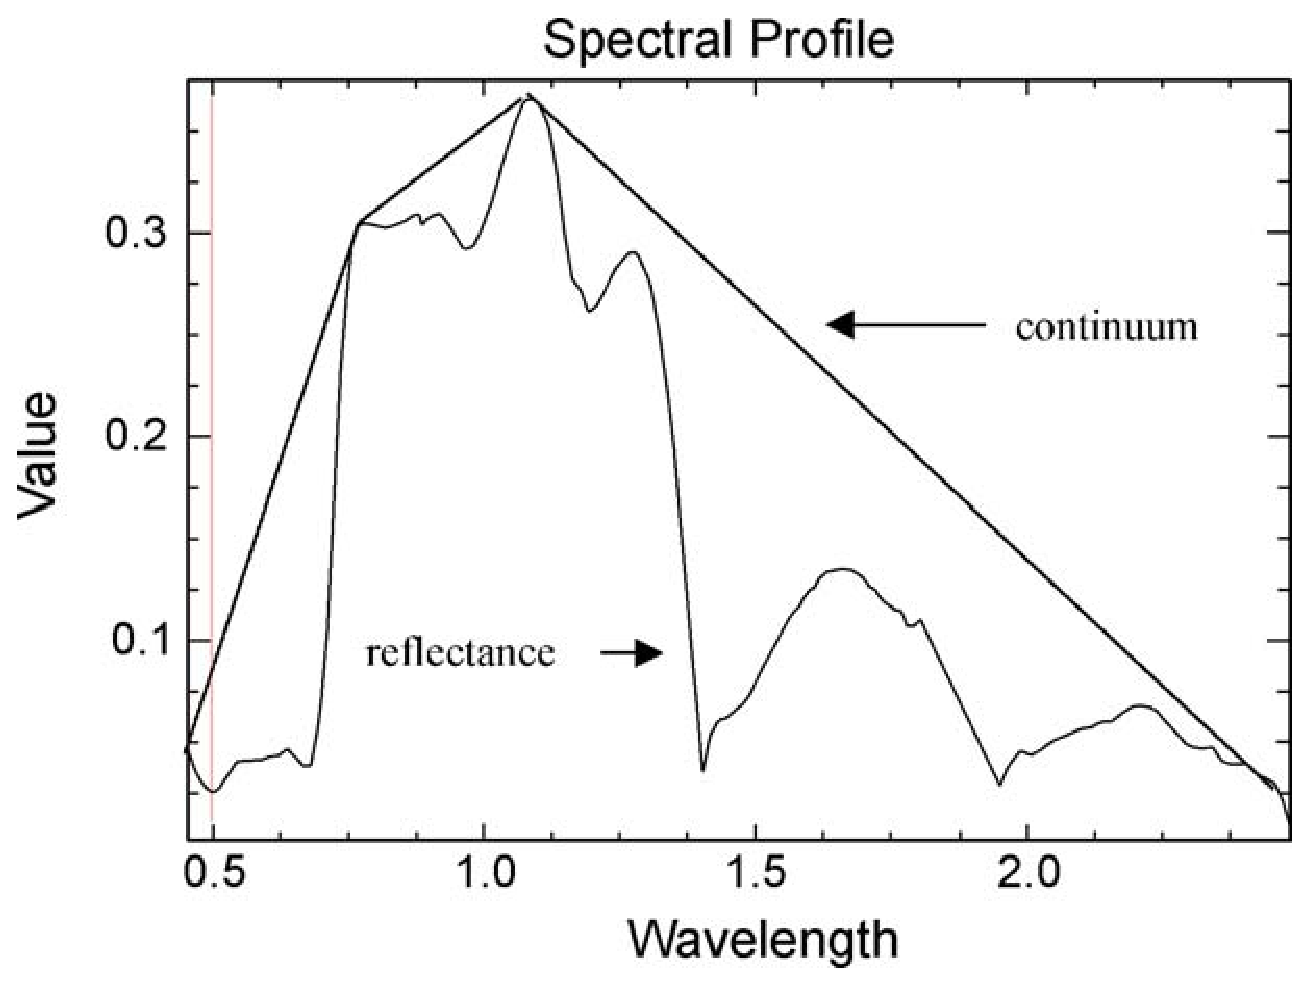
\includegraphics[width=0.5\linewidth]{./Imagenes/CR1.eps}
	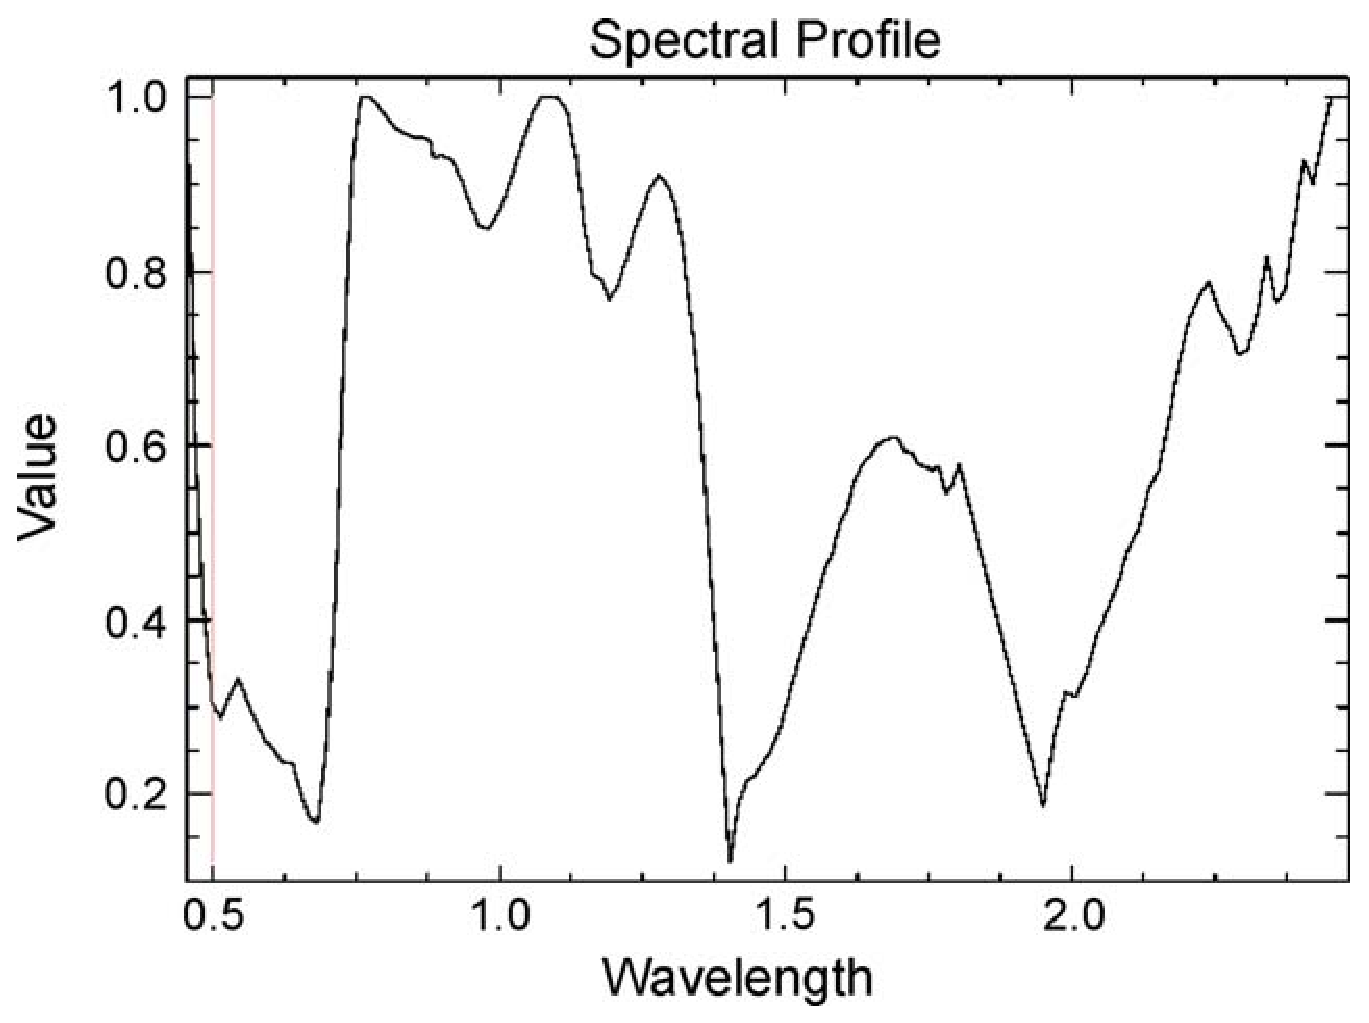
\includegraphics[width=0.5\linewidth]{./Imagenes/CR2.eps}
	\captionsetup{font={footnotesize,it}}
	\caption[Continuum Removal ejemplo]{Ejemplo de aplicación de la técnica continuum removal. Fuente:\cite{huang2004estimating}.}
	\label{fig:ejemploCR}
\end{figure}

Este método no aporta un valor numérico de cuantificación de la similitud entre dos espectros, centrándose en un análisis gráfico de cada respuesta por separado.%\Sep

El paquete base de R ya incluye las operaciones estadísticas básicas necesarias para la elaboración de la clasificación angular y el \ac{IAE} con la única excepción de que para poder aplicar el analizador \ac{CR} se debe descargar el paquete adicional \textit{prospectr} \citep{stevens2014introduction}.%\Sep

En la figura \ref{fig:CR} se muestra el script original de la función en R a la que se le aplicarán los datos de campo y que devuelve la gráfica de \ac{CR}.%\Sep

\begin{figure}
\centering
\begin{lstlisting}[language = R]
  require(prospectr) # carga del paquete necesario
  
  # aplicacion de la funcion implementada en prospectr 
  cr <- continuumRemoval(mangle1corte$V5, mangle1corte$V4,
                         type="R",
                         interpol="linear")
                         
  grafica(data1) # salida grafica a los datos iniciales
  lines(data1$V4,cr) # superposicion de la grafica de CR
\end{lstlisting}
\captionsetup{font={footnotesize,it}}
\caption[Función de \textit{Continuum Removal}]{Script de la función de \textit{Continuum Removal} en R. Elaboración propia a partir de \cite{stevens2014introduction}.}
\label{fig:CR}
\end{figure}

Se puede observar como mediante el comando inicial \textit{require()} se llama al paquete \textit{prospectr}, gracias al cual nos aseguramos que está correctamente cargado el paquete necesario para realizar las operaciones que siguen en el script \citep{stevens2014introduction}. Para ello se utilizó el instalador de paquetes de RStudio, localizando el paquete requerido en el repositorio oficial de RCRAN e instalando las dependencias necesarias, que también se podría haber hecho con el comando \textit{``install.packages()''}. El comando \textit{grafica()} es la llamada a una función creada para presentar la gráfica a nuestro gusto, mientras que con el comando \textit{lines()} se nos permite superponer la gráfica de \ac{CR} a la anterior.%\Sep

Para el correcto funcionamiento del análisis se procedió a crear una matriz de 3x481 donde las filas corresponden a las tres especies analizadas y las columnas al valor de longitud de onda. El fin es el de presentar de mejor forma los datos en la función de \ac{CR} de R y aunque el resultado es el mismo, que haciéndolo una por una, nos permite obtener este de forma más rápida y con menos pasos.%\Sep

El script original de la funcion en R previamente presentado en la figura \ref{fig:CR} sufre cambios, quedando de la siguiente manera:%\SmallSep

\begin{figure}[ht]
	\centering
	\begin{lstlisting}[language = R]
  require(prospectr)
  
  # generacion de la matriz de datos
  matriz <- matrix(c(RhizophoraCorte$V5,LagunculariaCorte$V5,
                     AvicenniaCorte$V5),
                   byrow=TRUE,
                   nrow=3,
                   ncol=481)
  
  # se especifica el numero de observaciones                 
  bandas <- mangle1corte$V4
  
  # se aplica la funcion
  cr <- continuumRemoval(matriz, bandas)
  
  # salida grafica a los datos
  matplot(bandas, t(matriz),
          type="l", ylim=c(0,1))
  matlines(bandas, t(cr2))
	\end{lstlisting}
	\captionsetup{font={footnotesize,it}}
	\caption[Función modificada de \textit{Continuum Removal}]{Script modificado de la función de \textit{Continuum Removal} escrita en R. Elaboración propia.}
	\label{fig:CRmodificado}
\end{figure}	

Donde ``manglencorte'' es el archivo de datos con el corte realizado para cada especie como se explicó anteriormente. Se crea un objeto llamado ``bandas'' tomando los valores de la fila V4 de cualquiera de los archivos de datos. Se crea la gráfica con el comandos \textit{matplot()} y con \textit{matlines()} se superpone la gráfica propia del método \ac{CR}.%\Sep

\subsection{Clasificación angular}
La clasificación angular también llamada \ac{SAM} calcula la similitud entre dos espectros a partir de su distancia angular espectral. Originalmente este método compara espectros desconocidos con otros de referencia tomados, por ejemplo, de bibliotecas espectrales o de la misma imagen \citep{girouard2004validated} con el fin de asignar píxeles desconocidos a clases de referencia conocida en una clasificación temática. El algoritmo de clasificación angular es el siguiente:

\begin{equation} \label{eq:angular}
	\theta = arcos \frac{\sum_{k=1}^{m} \rho_{i,k} \rho_{j,k}}{\sqrt{\sum_{k=1}^{m} \rho_{i,k}^{2}} \sqrt{\sum_{k=1}^{m} \rho_{j,k}^{2}}}
\end{equation}%\Sep

Siendo $\rho_{i,k}$ la reflectividad del espectro \textit{i} en una banda \textit{k}, $\rho_{j,k}$ la reflectividad del espectro \textit{j} en la misma banda y \textit{m} el número de bandas.%\Sep

Los espectros serán más similares cuanto menor sea el valor del ángulo $\theta$ de la ecuación \ref{eq:angular}.%\Sep

En la figura \ref{fig:AE} se muestra el script de la función en R a la que se le aplicarán los datos de campo y que devuelve el valor del ángulo $\theta$.

\begin{figure}
\centering
\begin{lstlisting}[language = R]
  AE <- function(i,j) {
  
    Ri = i$V5 # valores de las observaciones
    Rj = j$V5
  
  # calculo del angulo espectral para dos cubiertas
    angulo = acos (sum(Ri*Rj)/(sqrt(sum(Ri^2))*sqrt(sum(Rj^2))))
    return(angulo)
  }
\end{lstlisting}
\captionsetup{font={footnotesize,it}}
\caption[Función clasificación angular]{Función de clasificación angular en R. Elaboración propia.}
\label{fig:AE}
\end{figure}

\section{Imágenes de satélite}
\subsection{Landsat 8}\label{subsec:Landsat8}
Landsat 8 dispone de 11 bandas espectrales: 9 del sensor \ac{OLI} (expuestas en la tabla \ref{tab:sensoresOLI}) y 2 del sensor \ac{TIRS} que no son de interés para este trabajo.%\Sep

Como los datos del radiómetro de campo solo abarcan las longitudes de onda comprendidas entre $325 nm$ y $1075 nm$ solo son de interés las cinco primeras bandas que se detallan a continuación:

\begin{itemize}
	\item Banda 1 (Coastal/Aerosol) [430-450 nm]: Detecta azules y violetas intensos. Solventa los problemas de la dispersión de Rayleigh. Facilita la detección de la calidad de aguas poco profundas y partículas de polvo o aerosol en la atmósfera.
	\item Banda 2 (Blue) [450-510 nm]: Detecta el azul del espectro visible. Útil para diferenciar el suelo desnudo de la vegetación y detectar zonas pavimentadas como carreteras o áreas urbanas.
	\item Banda 3 (Green) [530-590 nm]: Detecta el verde del espectro visible. Sensible al nivel de turbidez del agua. Brillante en zonas de tierra árida y oscura en zonas boscosas o de cultivos.
	\item Banda 4 (Red) [640-670 nm]: Detecta el rojo del espectro visible. Útil en la clasificación de zonas vegetales pero no diferencia estas de agua, puesto que aparecen como zonas oscuras.
	\item Banda 5 (NIR) [850-880 nm]: Detecta el infrarrojo cercano. Especialmente importante en ecología porque la vegetación vigorosa la refleja. Útil para la obtención del \ac{NDVI} y distinguir tipos de vegetación.
\end{itemize}


\subsection{Obtención de las imágenes}
Las imágenes se obtuvieron del servicio Earth Explorer, de la \ac{EROS} de la \ac{USGS}. Estas imágenes ya vienen con una corrección geométrica previa hecha, por lo que no será necesario aplicar más correcciones de este tipo. En un archivo .txt asociado a las imágenes .tiff para cada banda se especifica que el método de corrección geométrica utilizado ha sido el de convolución cúbica.%\Sep

En concreto, los archivos que nos ofrece el servicio de descargas son:

\begin{itemize}
	\item Una imagen en composición de color natural como las que se muestran en la figura \ref{fig:imagenesLandsat}.
	\item Una imagen térmica que no nos será de utilidad.
	\item Una imagen de 8 bits que cuantifica la calidad de la observación.
	\item Las imágenes anteriormente citadas georreferenciadas.
	\item Las imágenes correspondientes a cada banda de Landsat 8 con la corrección geométrica aplicada (level 1) en formato GeoTIFF.
\end{itemize}%\Sep

Se trata de un producto de \ac{L1T} con correcciones geométricas sistemáticas aplicadas utilizando para ello puntos de control terrestre o información de posición integrada a bordo \citep{Ariza2013}. Se entrega así una imagen registrada a la proyección WGS84. Adicionalmente en este nivel de producto contiene una corrección topográfica por el desplazamiento del terreno debido al relieve. Las imágenes se encuentran en formato de \ac{ND} que se pueden transformar a valores de reflectividad \ac{TOA} en las bandas 1 a 9.%\Sep

Otra forma de obtener las imágenes de Landsat 8 es mediante el gestor de descargas Libra, que aprovecha la API del servicio de \ac{AWS} que aloja estas imágenes desde septiembre de 2014. Este nos permite elegir que bandas descargar, ahorrando tiempo en la operación.%\Sep

En cambio, para la correcta realización de este \ac{TFG} donde tenemos datos de reflectividad a nivel del suelo, necesitamos que las imágenes Landsat también muestren valores de reflectividad a ese nivel. Esto se consigue aplicando un algoritmo de corrección radiométrica a las imágenes \ac{L1T} obteniendo un producto también proporcionado por la agencia \ac{EROS} bajo demanda llamado \ac{PL8SR} \citep{USGS2015} que también se puede encontrar bajo en nombre de Landsat SR.%\Sep

Para abarcar la zona de estudio se necesitaron obtener dos imágenes que tienen las características mostradas en el cuadro \ref{tab:imagenes}. Se consideró que la diferencia temporal entre ambas imágenes y la fecha de toma de datos no era determinante suponiendo un escaso cambio fenológico de las especies de mangle en ese periodo de tiempo.%\Sep

\begin{table}[ht]
	\centering
	\begin{tabular}{@{}cccccccc@{}}
	\toprule[0.4mm]
	Imagen & Path & Row & Fecha & West & East & North & South \\
	\midrule
	1 (a) & 18 & 51 & 23/11/2014 & -89.105062 & -86.987819 & 14.067713 & 11.946409 \\
	2 (b) & 17 & 51 & 19/12/2014 & -87.549399 & -85.443030 & 14.062287 & 11.952632 \\
	\bottomrule[0.4mm]
	\end{tabular}
	\captionsetup{font={footnotesize,it}}
	\caption[Caracerísticas de las imágenes Landsat]{Características de las imágenes Landsat obtenidas de la figura \ref{fig:imagenesLandsat}. Elaboración propia.}
	\label{tab:imagenes}
\end{table}

Se observa en las imágenes de calidad de la figura \ref{fig:imagenescalidad}, en las que las nubes y nubes altas se marcan de color blanco y amarillo respectivamente, que la cobertura nubosa es aceptable para trabajar en la zona de estudio.%\Sep

\begin{figure}
	\centering
	\subfloat[Imagen Landsat path 18 row 51 (23/11/14)]{
	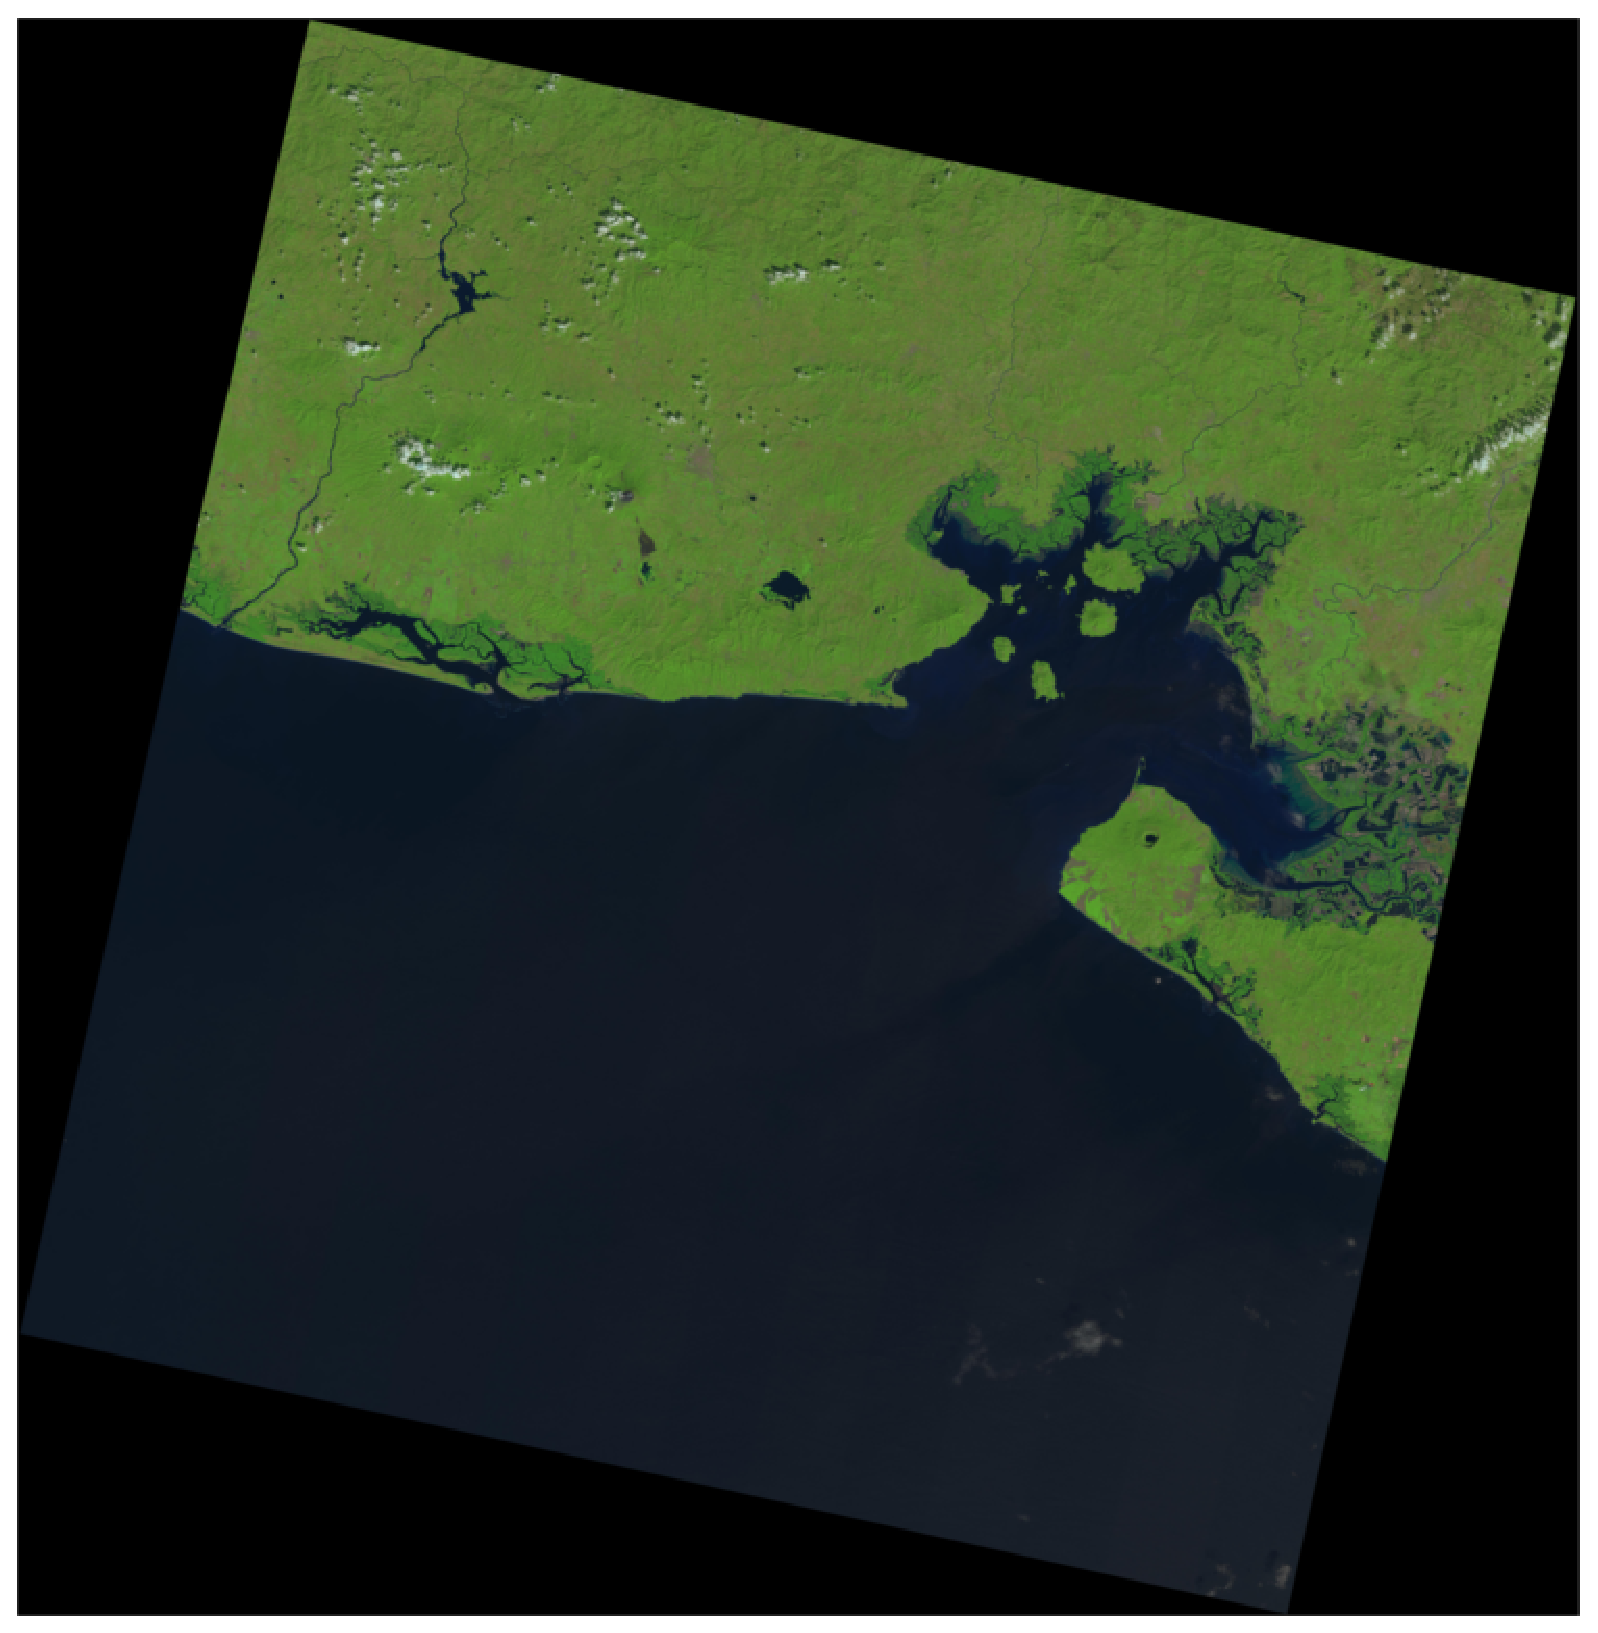
\includegraphics[width=0.45\linewidth]{./Imagenes/Landsat18.eps}}
	\subfloat[Imagen Landsat path 17 row 51 (19/12/14)]{
	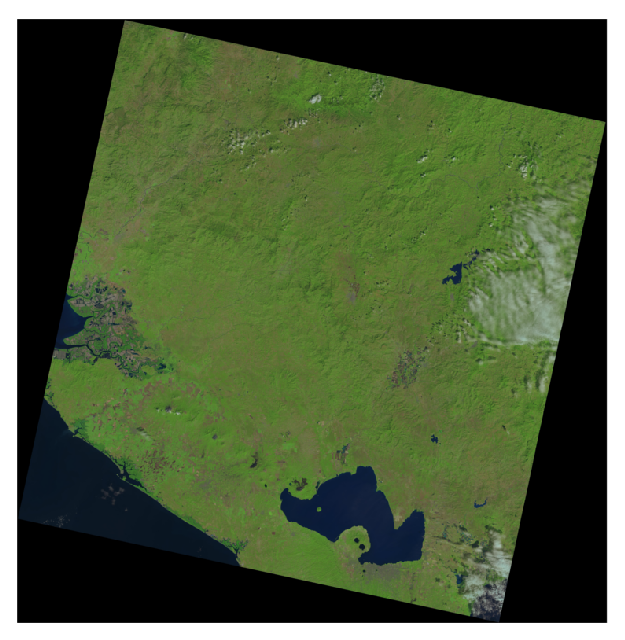
\includegraphics[width=0.45\linewidth]{./Imagenes/Landsat17.eps}}
	\captionsetup{font={footnotesize,it}}
	\caption[Imágenes Landsat]{Imágenes Landsat con corrección geométrica utilizadas para el trabajo. Fuente: USGS.}
	\label{fig:imagenesLandsat}
\end{figure}

\begin{figure}
	\centering
	\subfloat[Imagen de calidad Landsat path 18 row 51 (06/10/14)]{
	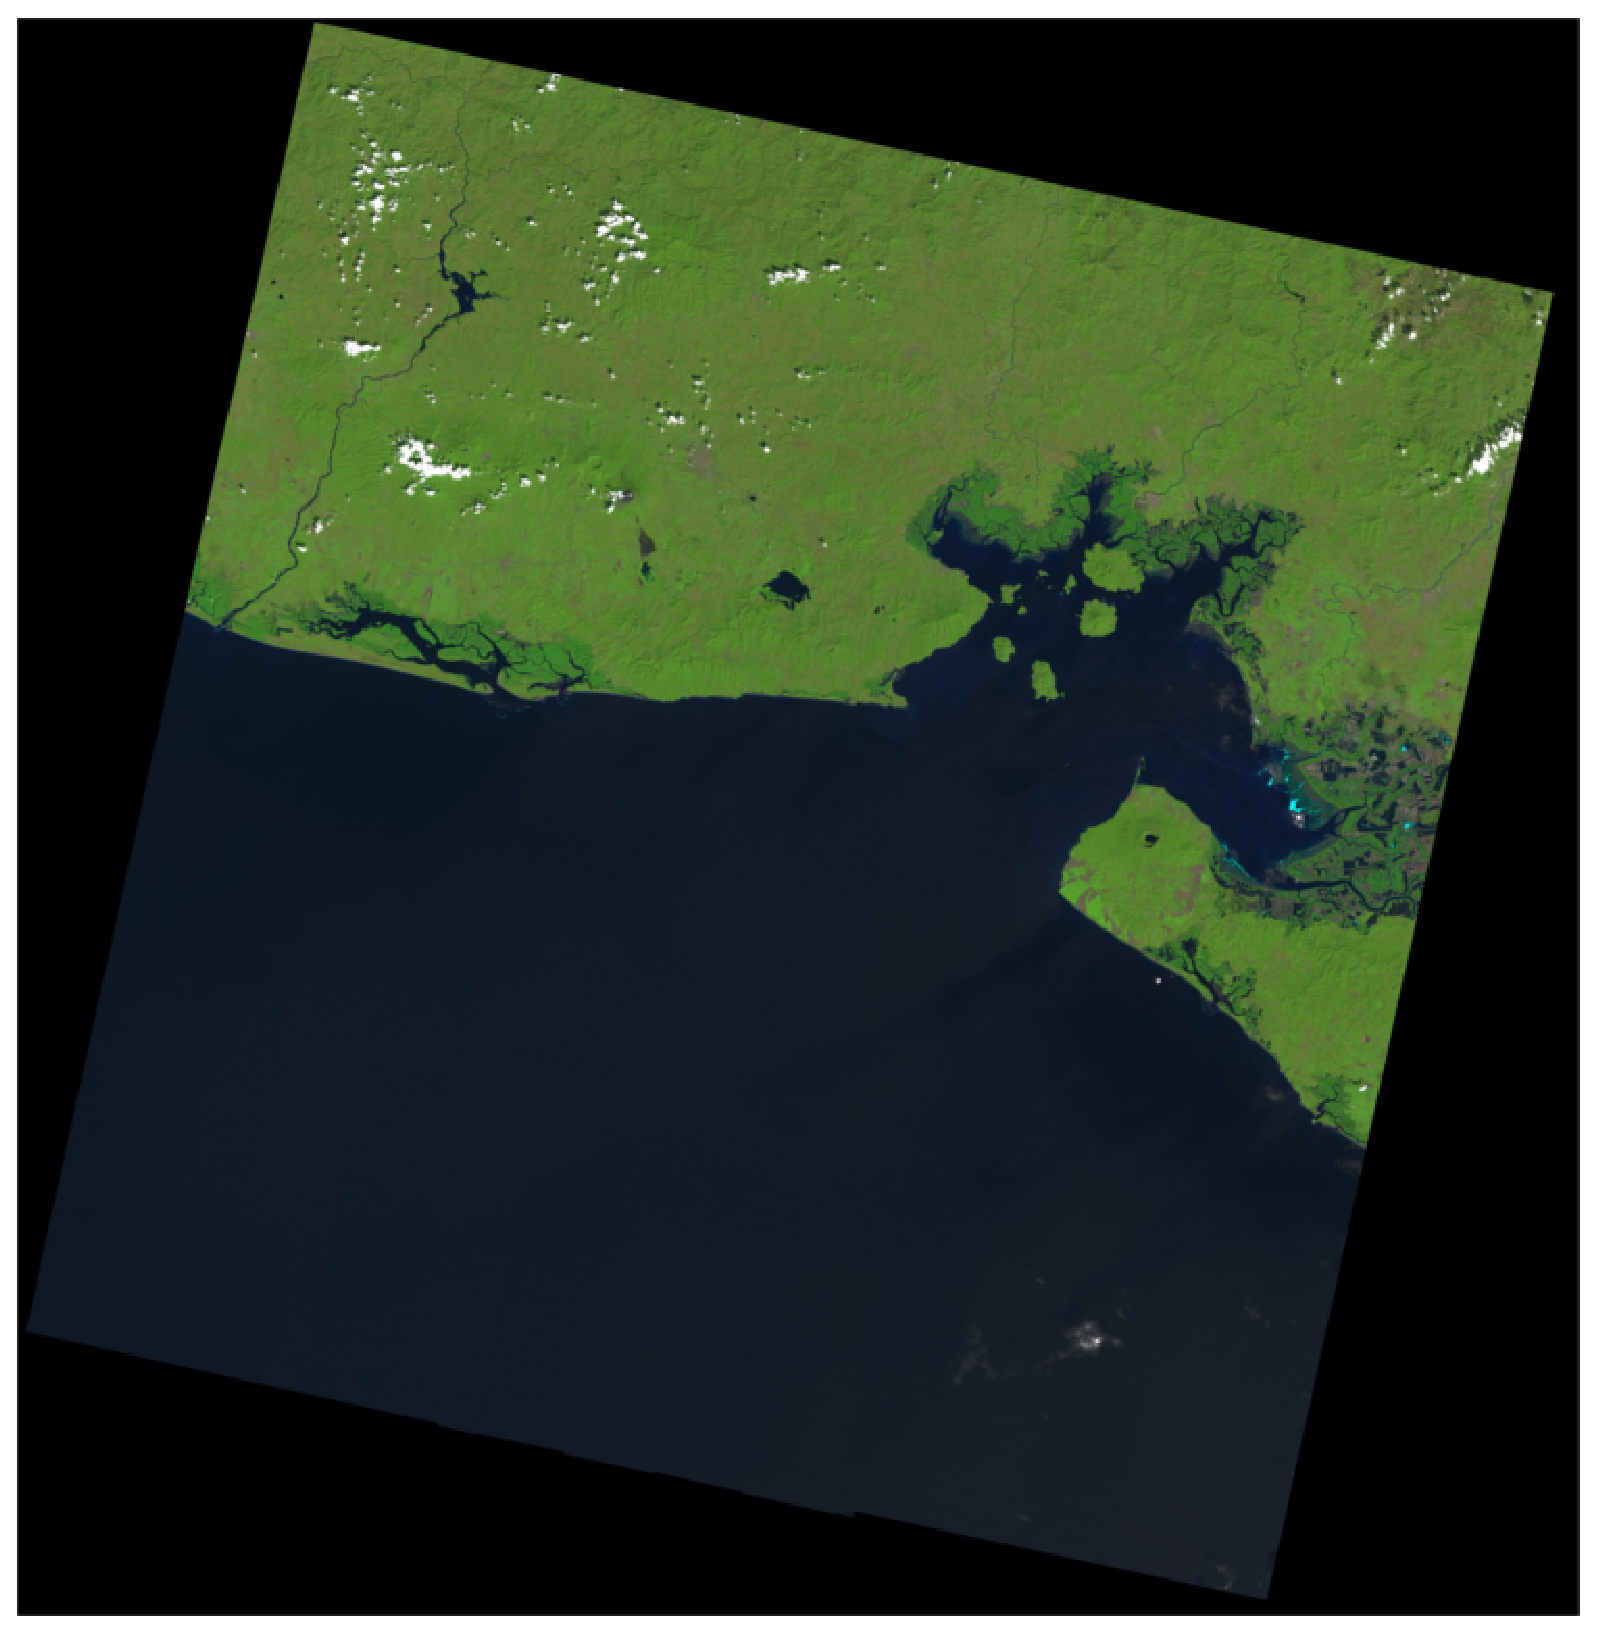
\includegraphics[width=0.45\linewidth]{./Imagenes/LandsatQ18.eps}}
	\subfloat[Imagen de calidad Landsat path 17 row 51 (16/11/14)]{
	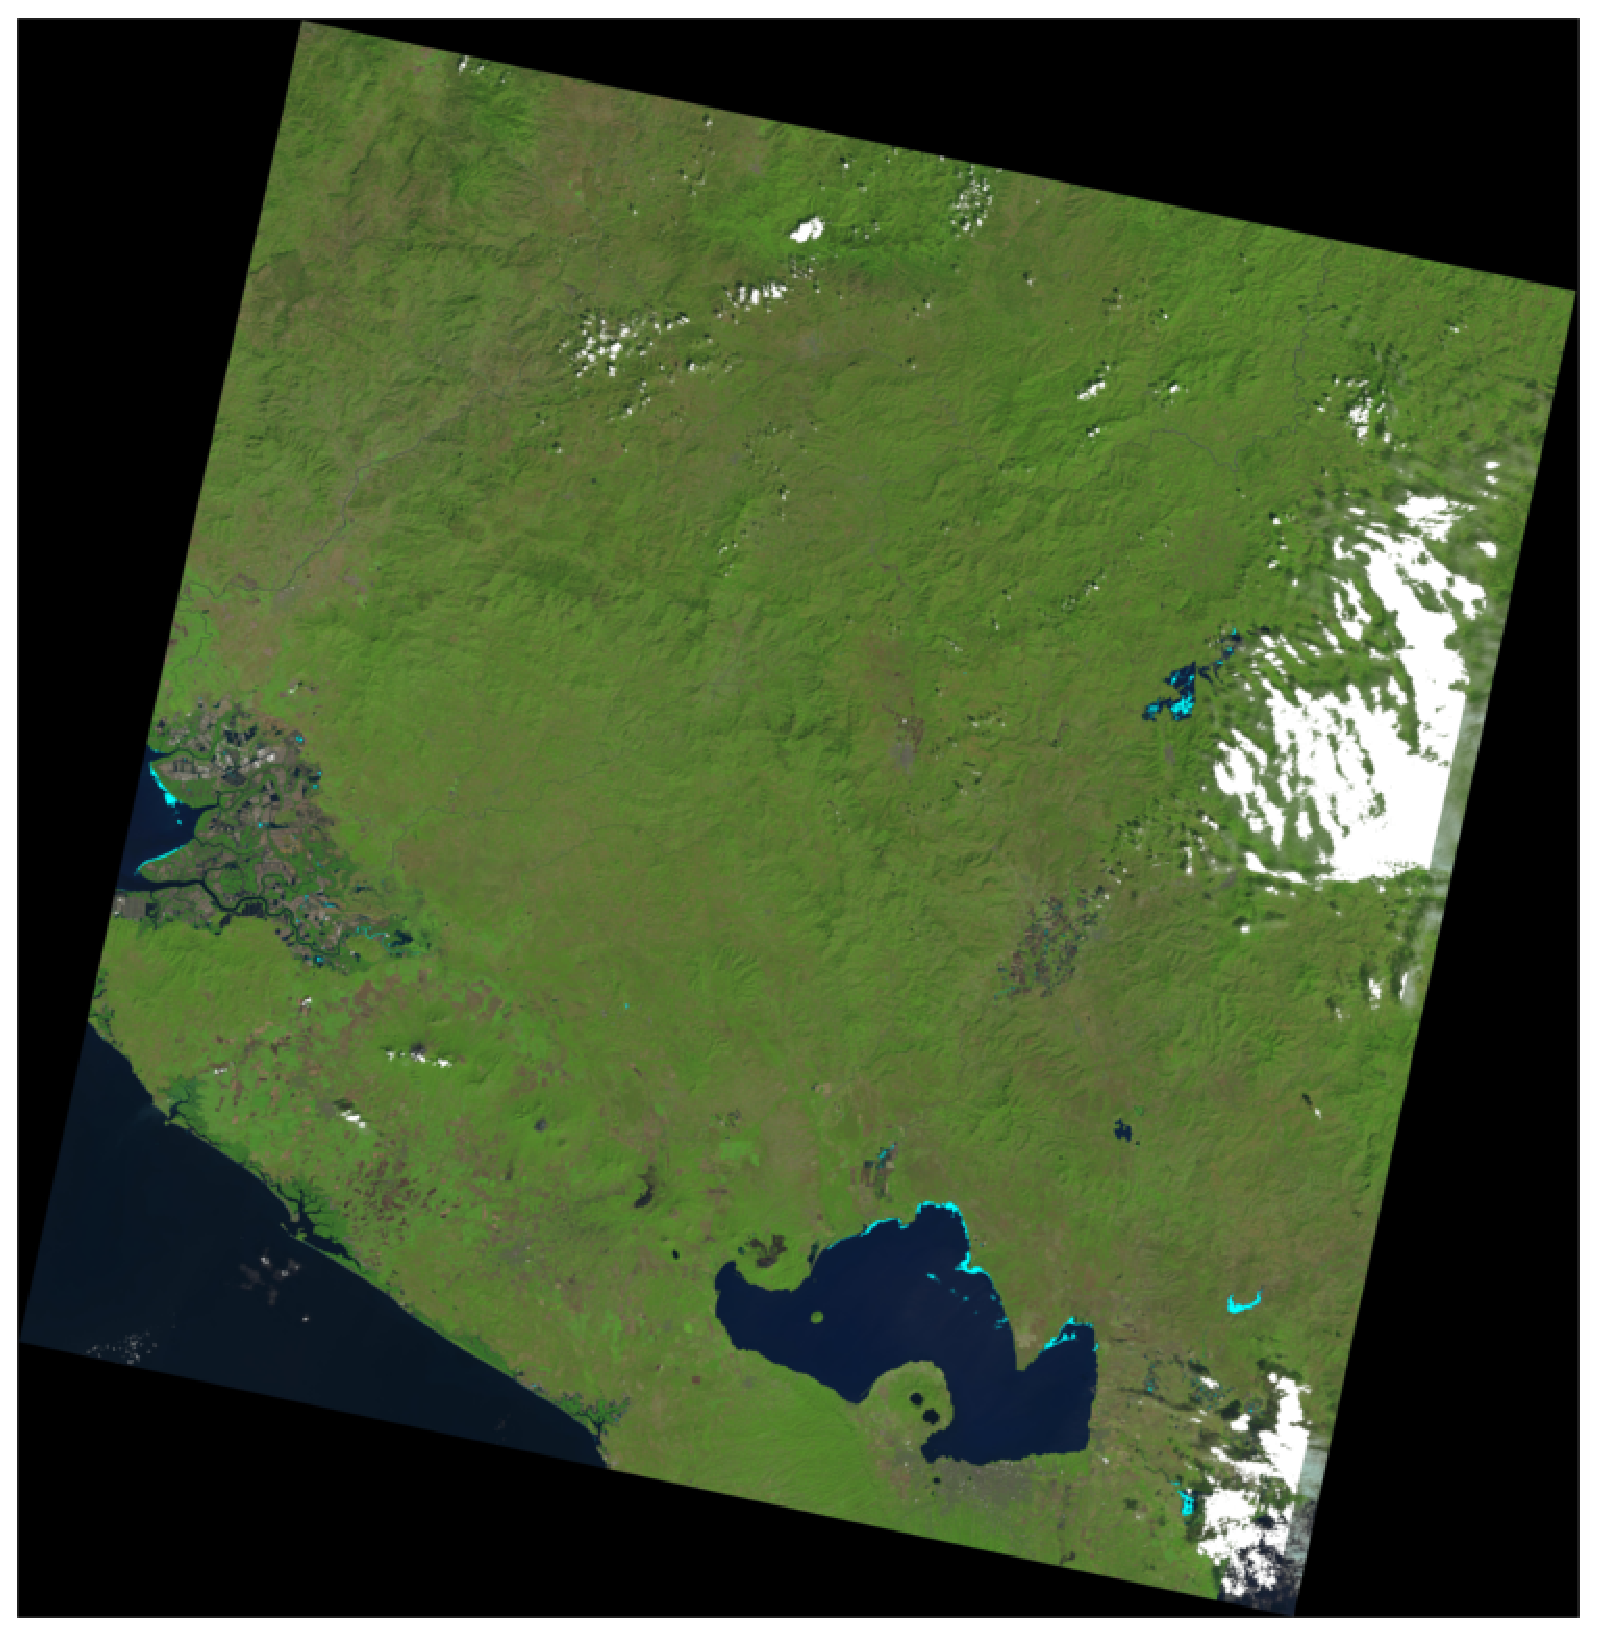
\includegraphics[width=0.45\linewidth]{./Imagenes/LandsatQ17.eps}}
	\captionsetup{font={footnotesize,it}}
	\caption[Imágenes de calidad de Landsat]{Imágenes de calidad de Landsat de 8 bits. Fuente: USGS.}
	\label{fig:imagenescalidad}
\end{figure}

Las imágenes utilizan el siguiente código de identificación en el nombre \citep{Ariza2013} \citep{USGS2015}:

\begin{center}
	\fbox{LXSPPPRRRYYYYDDDGSIVV}
\end{center}

\noindent donde:

\begin{itemize}
	\item L: Landsat.
	\item X: Sensor.
	\item S: Satélite.
	\item PPP: Path.
	\item RRR: Row.
	\item YYYY: Año de adquisición de la imagen.
	\item DDD: Día juliano del año.
	\item GSI: Identificador de la estación terrestre de seguimiento.
	\item VV: Versión del archivo.
\end{itemize}

\subsection{Tratamientos previos}
Como se decía en el apartado anterior, la geometría de las imágenes ya está corregida. Pero es necesario realizar algunos procedimientos antes de unirlas y recortarlas finalmente para que se adapten a la zona de estudio y sea más cómodo trabajar con ellas. Estos procedimientos son el tratamiento de los valores nulos, la transformación de los \ac{ND} en reflectancias, el mosaico de imágenes, su posterior recorte y la aplicación de un filtro de paso bajo.%\Sep

Lo primero que se debe hacer en GRASS es crear la localización \textit{(location)} de nuestro proyecto y añadir las imágenes al directorio de mapas \textit{(mapset)}. Los datos de la localización se establecen gracias a la lectura por parte de GRASS de la configuración de proyección y datum de un archivo de datos georreferenciado, es decir, de cualquier imagen de Landsat del trabajo. Las imágenes se añadirán al \textit{mapset} con el comando \textit{r.in.gdal}.

\subsubsection{Valores nulos}
El tratamiento de los valores nulos se lleva a cabo mediante el comando \textit{r.null} como sigue:

\begin{figure}[ht]
\centering
\begin{boxedverbatim}
	r.null map=LC80180512014279LGN00_B1@TFG setnull=0 null=-9999
\end{boxedverbatim}
\captionsetup{font={footnotesize,it}}
\caption[Valores nulos]{Tratamiento de valores nulos en GRASS con el comando \textit{r.null}.}
\end{figure}

\noindent donde \textit{``map''} corresponde a la banda a tratar seguido por el \textit{mapset}, \textit{``setnull''} indica el valor de los elementos nulos y \textit{``null''} indica el nuevo valor de estos elementos. Se elige un valor de -9999 para evitar posibles errores de realizarse, por ejemplo un \ac{NDVI} que trabaja con valores de píxel de [-1,1].%\Sep

Este no es un procedimiento obligatorio aunque recomendable ya que los geoprocesos aplicados siguientes, como el mosaico de imágenes, ya implican un tratamiento de valores nulos.

%\subsubsection{Transformación a reflectancias}
%Los \ac{ND} pueden ser reescalados a valores de reflectancias \ac{TOA} gracias a los coeficientes radiométricos provistos en el archivo .txt que acompaña a las imágenes. Esta transformación se hará con el comando \textit{i.landsat.toar} como sigue:

%\begin{figure}[ht]
%\centering
%\begin{boxedverbatim}
%	i.landsat.toar
%	input_prefix=LC80170512014320LGN00_B
%	output_prefix=LC80170512014320LGN00_TOAR_B
%	metfile=/home/marcos/grassdata/Imagenes/Landsat/
%	P17R51/Base/LC80170512014320LGN00_MTL.txt
%	sensor=oli8
%	method=dos4
%	date=2014-11-16
%	sun_elevation=52.01756824
%\end{boxedverbatim}
%\captionsetup{font={footnotesize,it}}
%\caption[Transformación a reflectancias]{Transformación a reflectancias TOA en GRASS con el comando \textit{i.landsat.toar}.}
%\end{figure}

%\noindent donde \textit{``input\_prefix''} es el prefijo del nombre de las imágenes para cada banda, \textit{``output\_prefix''} es el prefijo que le queremos dar a las nuevas imágenes corregidas, \textit{``metfile''} es el archivo de metadatos asociado, \textit{``sensor''} el tipo de sensor, \textit{``date''} es la fechas de adquisición y \textit{``sun\_elevation''} la elevación en grados del Sol.

\subsubsection{Mosaico de imágenes}
Para realizar el mosaico de las dos imágenes de las que disponemos tenemos dos opciones: utilizando la herramienta \textit{gdal\_merge.py} y hacerlo en GRASS. Para utilizar la herramienta de la librería \ac{GDAL} gdal\_merge.py debemos tener las siguientes consideraciones previas:

\begin{itemize}
	\item Es un método que se ejecuta en la terminal de Linux. Para un método guiado se utilizaría, por ejemplo, la herramienta \textit{raster/combinar} en QGIS o el método de GRASS que se expondrá más adelante.
	\item Las dos imágenes deben estar en el mismo sistema de coordenadas.
	\item Utiliza como método de remuestreo el de vecino más próximo.
	\item La última imagen de la lista será copiada sobre la precedente en el caso de haber solape.
\end{itemize}

La línea de comando en cuestión es la siguiente (para las imágenes de la primera banda y en el caso de tener situadas las imágenes en la misma carpeta):

\begin{figure}[ht]
\centering
\begin{boxedverbatim}
	gdal_merge.py -n 0 -v LC80170512014320LGN00_B1.TIF 
	LC80180512014279LGN00_B1.TIF -o mosaico1.tif
\end{boxedverbatim}
\captionsetup{font={footnotesize,it}}
\caption[Mosaico de imágenes]{Mosaico de imágenes con herramientas GDAL.}
\end{figure}

En este caso se utilizan los comandos asociados u opciones siguientes: -n para que se ignoren los píxeles con valores nulos, -v para que se detallen las operaciones realizadas y -o que permite dar nombre al archivo de salida. Con este método no sería necesario realizar el tratamiento de valores nulos.%\Sep

En la figura \ref{fig:dialogomosaico} se observa el diálogo resultante de la operación anterior que confirma que se ha hecho bien el mosaico. En el tenemos datos de las imágenes como el nombre, las coordenadas de la esquina superior izquierda e inferior derecha, tamaño del píxel y tiempo que se necesitó para realizar la operación.%\Sep

\begin{figure}
	\centering
	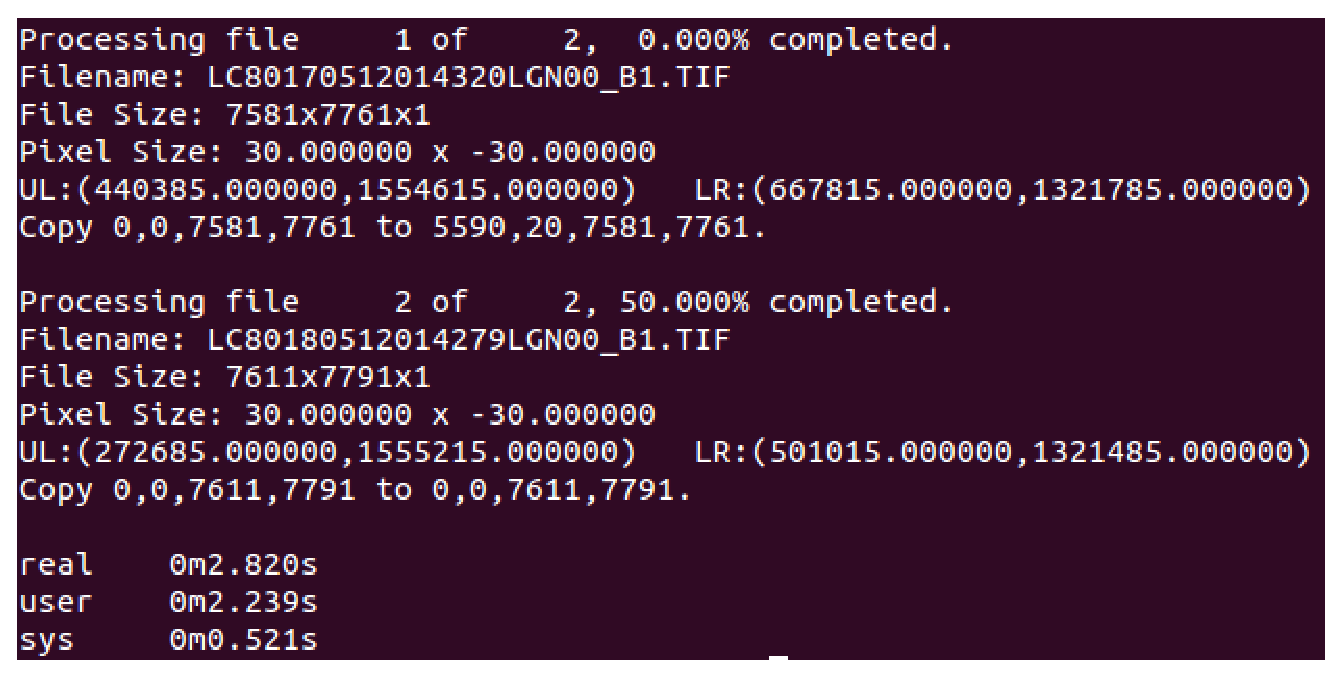
\includegraphics[width=0.8\linewidth]{./Imagenes/Dialogo_mosaico.eps}
	\captionsetup{font={footnotesize,it}}
	\caption[Diálogo del mosaicado]{Diálogo resultante del mosaicado de las imágenes en la terminal de Linux. Elaboración propia.}
	\label{fig:dialogomosaico}
\end{figure}

De hacerlo en GRASS, el comando sería \textit{r.patch}, con la salvedad de que las dos imágenes deben estar en la misma región de cálculo, la cual se puede ver en el cuadro \ref{tab:region}, quedando la línea de orden de la figura \ref{fig:rpatch}.

\begin{figure}[ht]
\centering
\begin{boxedverbatim}
	r.patch input=LC80180512014327LGN00_sr_band1@TFG,
	              LC80170512014352LGN00_sr_band1@TFG 
	output=Mosaico_B1
\end{boxedverbatim}
\captionsetup{font={footnotesize,it}}
\caption[Mosaico de imágenes en GRASS]{Mosaico de imágenes en GRASS mediante el comando \textit{r.patch}.}
\label{fig:rpatch}
\end{figure}

\subsubsection{Recorte de la imagen}
Para trabajar solamente con la zona de estudio es necesario recortar la imagen o reducir la región de cálculo. Para ello empleamos las opciones de visualización de GRASS con una extensión de coordenadas superior derecha de (516000 , 1501230) e inferior izquierda de (377940 , 1412100) como se muestra en el cuadro \ref{tab:region}. Una vez fijada se selecciona la opción de zoom ``set computational region from display extent'' que simplemente reduce la región de cálculo previamente establecida a la extensión de la visualización actual y nos permite realizar operaciones en esta.%\Sep

\begin{table}[ht]
	\centering
	\begin{tabular}{@{}rcc@{}}
	\toprule[0.4mm]
	& Extensión original & Extensión reducida\\
	\midrule
	Proyección & 1 (UTM) & 1 (UTM) \\
	Zona & 16 & 16 \\
	Datum & WGS84 & WGS84 \\
	Elipsoide & WGS84 & WGS84 \\
	Norte & 1555215 &1501230 \\
	Sur & 1321485 & 1412100 \\
	Oeste & 272685 & 377940 \\
	Este & 667815 & 516000 \\
	Res. esp. vertical (m) & 30 & 30 \\
	Res. esp. horizontal (m) & 30 & 30\\
	Filas & 7791 & 2971 \\
	Columnas & 13171 & 4602 \\
	Celdas & 102615261 & 13672542 \\
	\bottomrule[0.4mm]
	\end{tabular}
	\captionsetup{font={footnotesize,it}}
	\caption[Datos de las regiónes de trabajo]{Datos de las regiónes de trabajo establecidas en GRASS.}
	\label{tab:region}
\end{table}

Con el comando \textit{r.resample} se hace el remuestreo mediante vecino más próximo del área del recorte permitiendo obtener la imagen final para cada banda. El comando se emplea de la siguiente forma para cada banda:

\begin{figure}[ht]
\centering
\begin{boxedverbatim}
	r.resample input=MosaicoB1@TFG output=L8GF_SRB1
\end{boxedverbatim}
\captionsetup{font={footnotesize,it}}
\caption[Recorte de la imagen]{Recorte de la imagen en GRASS con el comando \textit{r.resample}.}
\end{figure}

A la hora de nombrar la imagen resultante en el \textit{output} ya se busca un código que identifique fácilmente la imagen. En este caso L8GF quiere decir que se trata de una imagen Landsat 8 del Golfo de Fonseca exclusivamente, mientras que SRB1 quiere decir que se trata de una imagen con reflectividades a nivel de suelo de la banda 1.

\subsubsection{Filtro de paso bajo}
La aplicación de un filtro de media a la imagen Landsat de la zona de estudio permite eliminar ruido y disminuir contrastes \citep{aldalur2002}. Antes de aplicar el filtro conviene realizar una copia de seguridad de la imagen debido a que se van a modificar los valores de reflectividad originales. Para ello se emplea el comando \textit{r.out.gdal} que permite exportar las imágenes a formato GeoTIFF.%\Sep

Se aplica a la imagen la siguiente función en cada píxel:

\begin{equation}
	g(x,y)=\frac{1}{9} \cdot \left(\begin{array}{ccc}
								   	1&1&1\\
								   	1&1&1\\
							 	   	1&1&1
								   \end{array}
							 \right)
\end{equation}
\noindent donde $g(x,y)$ es el nuevo valor del píxel localizado en las coordenadas \textit{x} e \textit{y} de la imagen y la matriz refleja la dimensión 3x3 del filtro, afectando así a $g(x,y)$ solamente los valores de los píxeles vecinos.%\Sep

La operación es realizada en GRASS mediante el comando \textit{r.neighbors} como sigue:

\begin{figure}[ht]
\centering
\begin{boxedverbatim}
	r.neighbors input=L8GF_SRB1@TFG output=L8GF_SRFB1 size=3
\end{boxedverbatim}
\captionsetup{font={footnotesize,it}}
\caption[Filtro de paso bajo]{Filtro de paso bajo en GRASS con el comando \textit{r.neighbors}.}
\end{figure}

El comando admite varias operaciones de filtrado como entre otras: media, mediana y moda. Al no especificar ninguna opción extra en el comando más que el tamaño de matriz de filtrado que se aplica, GRASS aplica el método de media por defecto. En el código de nombre de la imagen se va a añadir una F para indicar que las imágenes están filtradas.

El resultado de estos tratamientos se puede ver en las figuras \ref{fig:gf432} y \ref{fig:gf543}.
\begin{figure}
	\centering
	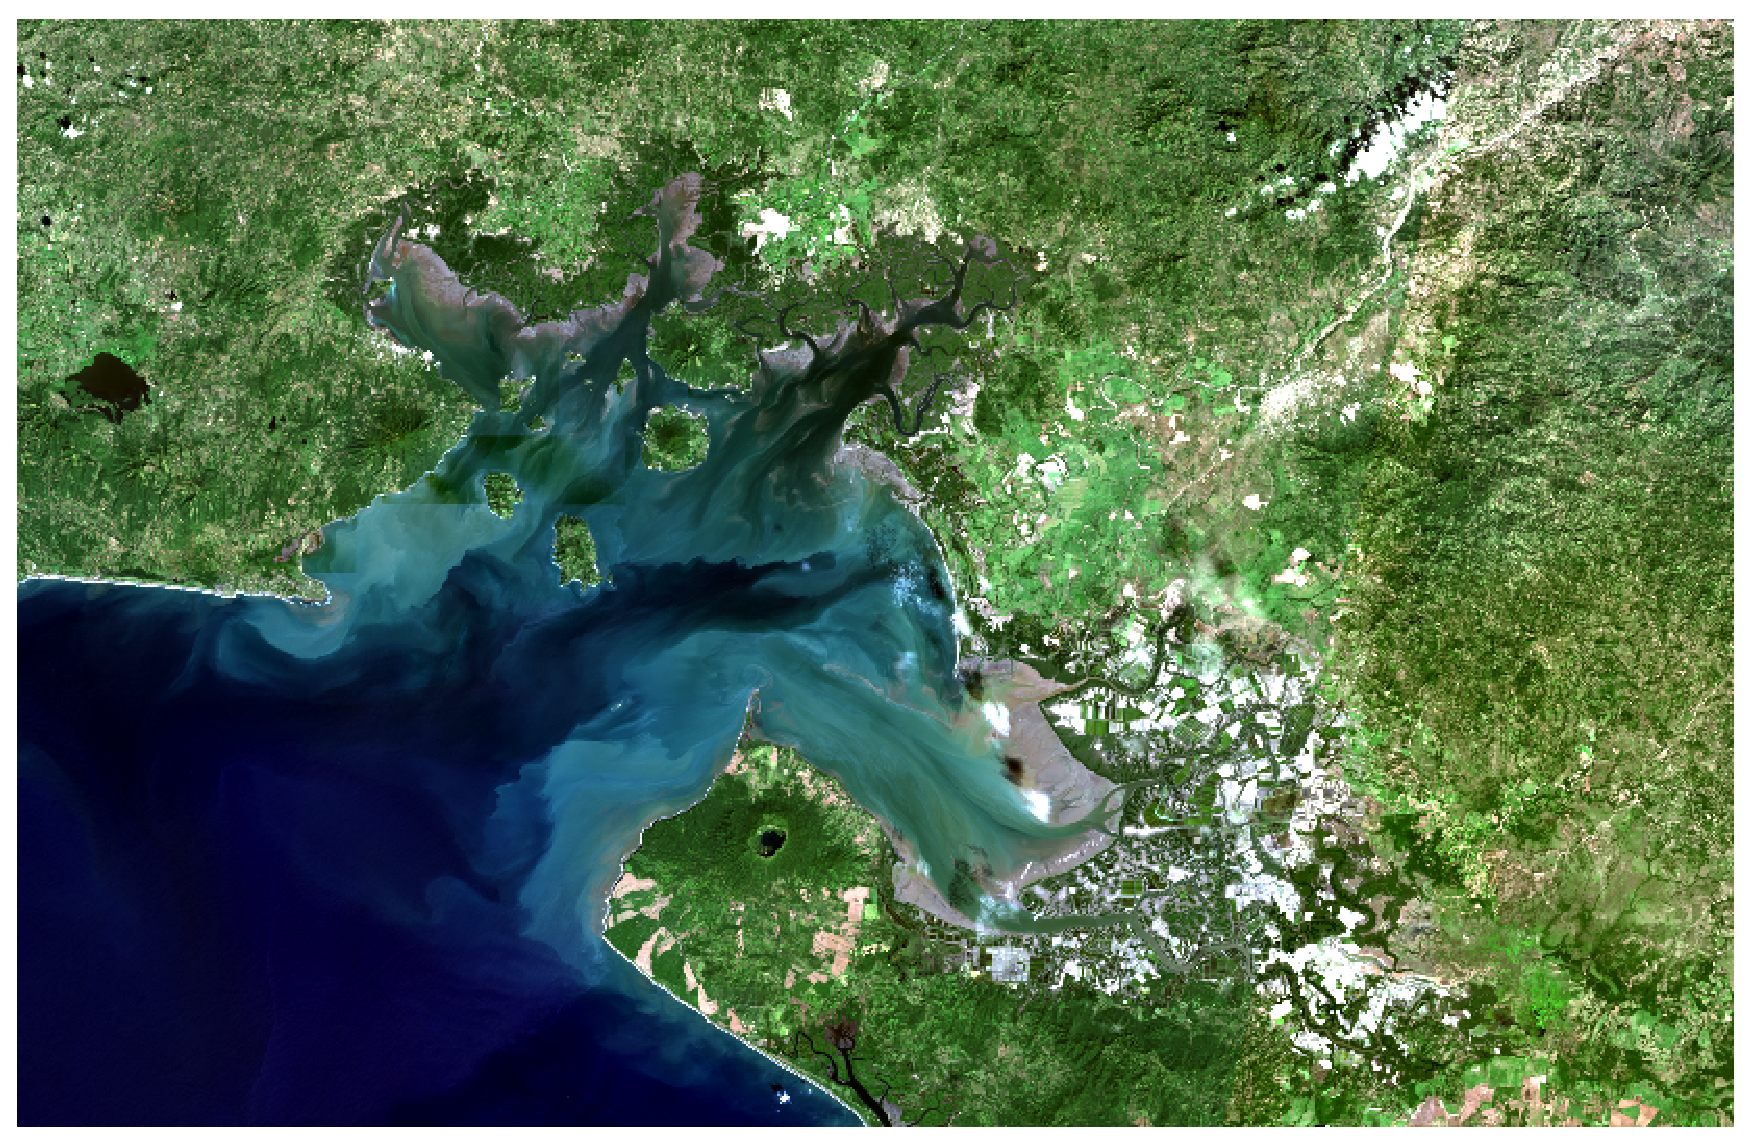
\includegraphics[width=0.9\linewidth]{./Imagenes/GF432.eps}
	\captionsetup{font={footnotesize,it}}
	\caption[Composición en color real]{Resultado de la imagen en una composición de color real (4-3-2). Imagen exportada de GRASS. Elaboración propia.}
	\label{fig:gf432}
\end{figure}

\begin{figure}
	\centering
	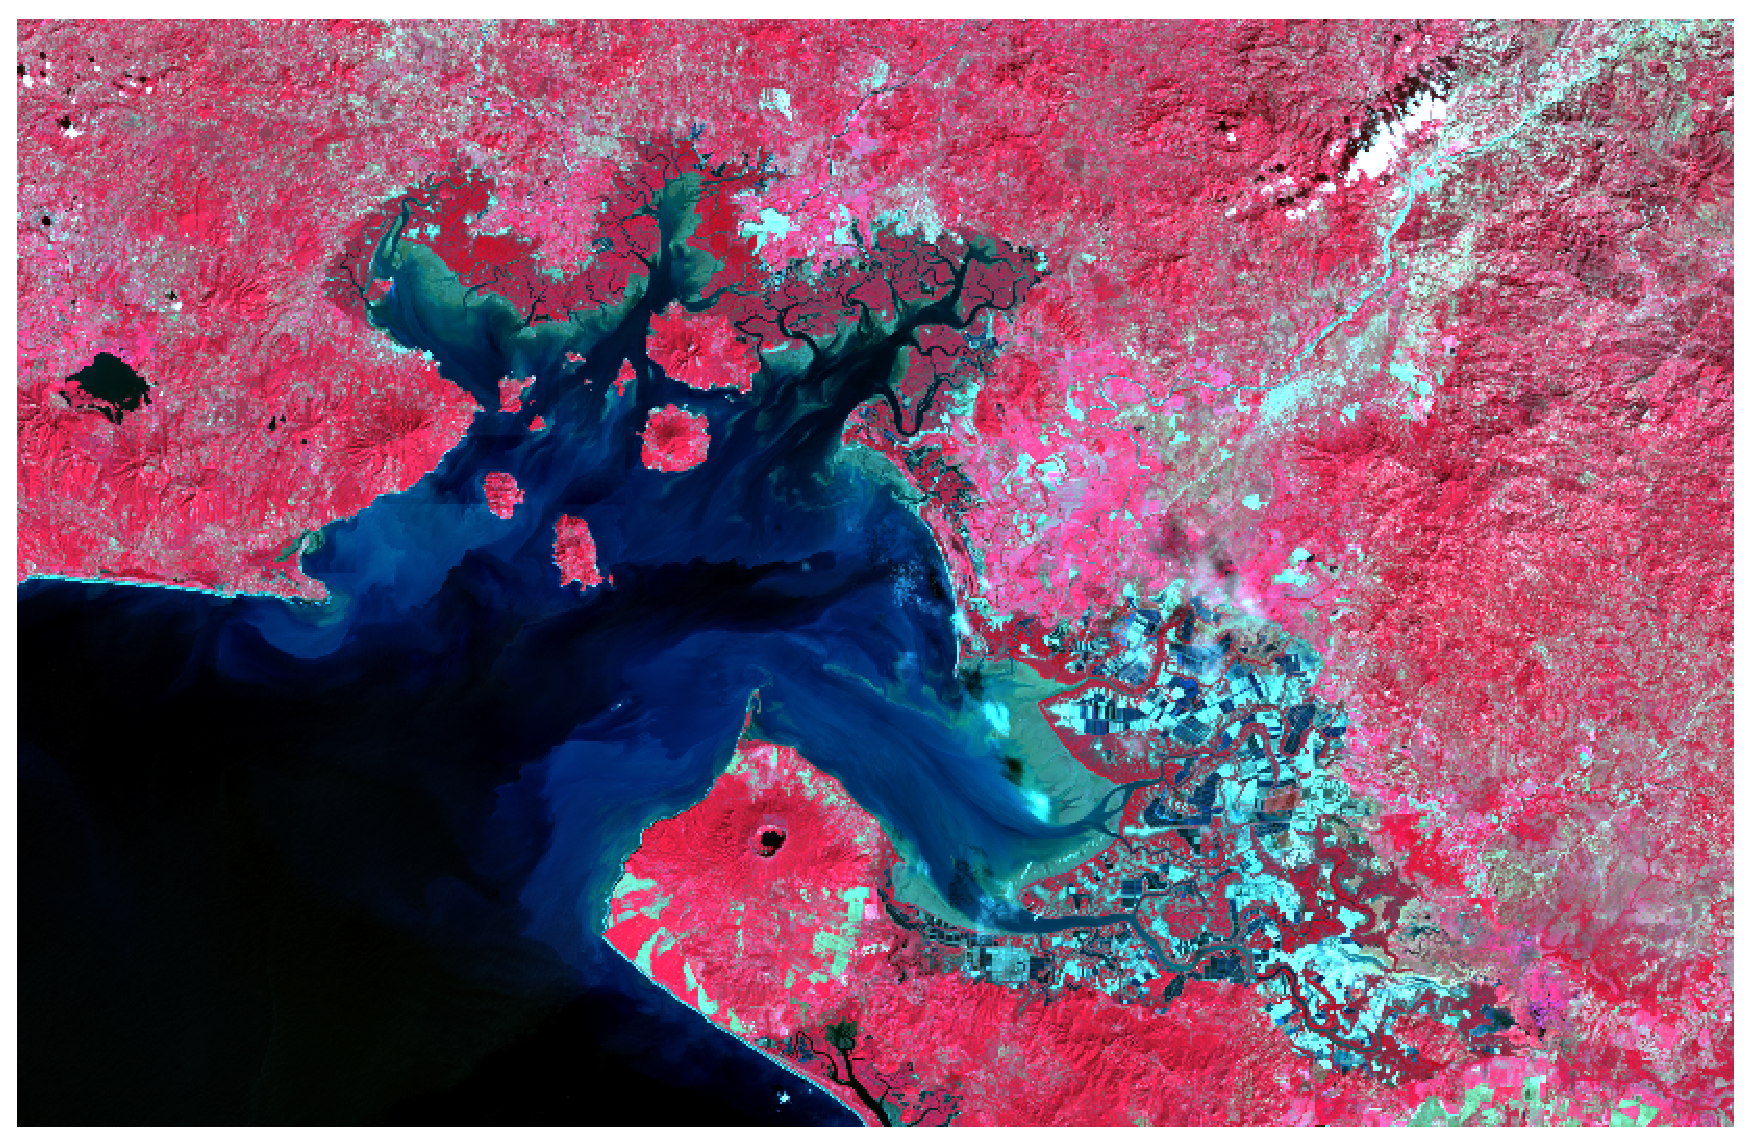
\includegraphics[width=0.9\linewidth]{./Imagenes/GF543.eps}
	\captionsetup{font={footnotesize,it}}
	\caption[Composición en falso color]{Resultado de la imagen en una composición de falso color (5-4-3). Imagen exportada de GRASS. Elaboración propia.}
	\label{fig:gf543}
\end{figure}

\section{Comprobación}
Debemos saber si los datos de reflectividad de las especies de mangle se adaptan a los datos de las imágenes raster de Landsat 8 que se han corregido. Para ello tomamos la serie de puntos en los que se conoce la existencia de bosque de mangle (cuadro \ref{tab:puntos}). Se creará en GRASS una capa vectorial con estos puntos a las que se le añadirán los valores raster de reflectividad de cada banda. Los pasos a seguir fueron los siguientes:

\begin{itemize}
	\item Creación de una capa vectorial en blanco de nombre ``puntos'' y añadirla al árbol de capas. En esta capa se digitalizarán un total de 10 puntos en los que se supone la existencia de bosque de mangle.
	\item Crear una base de datos asociada a la capa con \textit{v.db.addtable} asignando nuevos campos: ``x'' e ``y'' de tipo ``double'' que se actualizarán con las coordenadas de los puntos. También se añadirán a la tabla columnas para alojar el valor de los datos de cada una de las bandas en cada punto nombradas como B1, B2, B3, B4 y B5 de tipo ``double''.
	\item Actualización de los campos de coordenadas mediante el comando \textit{v.to.db} como se muestra en la figura \ref{fig:v.to.db} donde \textit{map} designa el vectorial que tiene la tabla asociada, \textit{option} indica que queremos actualizar coordenadas y \textit{columns} son los nombres de las columnas de coordenadas de nuestra tabla.
	
\begin{figure}[ht]
\centering
\begin{boxedverbatim}
	v.to.db map=puntos@TFG option=coor columns=x,y
\end{boxedverbatim}
\captionsetup{font={footnotesize,it}}
\caption[Actualización de coordenadas]{Actualización del campo coordenadas en GRASS con el comando \textit{v.to.db}.}
\label{fig:v.to.db}
\end{figure}	
	
	\item Actualización de los campos de datos del raster mediante el comando \textit{v.what.rast} como se muestra en la figura \ref{fig:v.what.rast} donde \textit{vector} indica cual es el vectorial que deseamos actualizar, \textit{raster} es el raster del que se tomarán los datos y \textit{column} el nombre del campo a actualizar.
\end{itemize}

\begin{figure}[ht]
\centering
\begin{boxedverbatim}
	v.what.rast vector=puntos@TFG raster=L8GF_SRFB1@TFG column=B1
\end{boxedverbatim}
\captionsetup{font={footnotesize,it}}
\caption[Actualización de los datos raster]{Actualización de los campos de datos raster en GRASS con el comando \textit{v.what.rast}.}
\label{fig:v.what.rast}
\end{figure}

\section{Clasificación de imágenes}
Con las figuras \ref{fig:gf432} y \ref{fig:gf543} del apartado anterior, composiciones en color real y falso color respectivamente, se puede observar como efectivamente el bosque de mangle se sitúa a lo largo de toda la costa del golfo adentrándose unos kilómetros al interior. Lo que se busca con la clasificación es reafirmar este hecho así como detectar de forma más clara esas zonas donde la proliferación de estanques de cría de camarón y salineras están afectando al ecosistema del manglar.%\Sep

Puesto que los datos disponibles no permiten la aplicación de un clasificador como el de paralelepípedos, ideal para utilizar valores estadísticos extraídos del análisis de datos, se procedió a emplear el \ac{MLC} para una clasificación supervisada y no supervisada y el clasificador \ac{SAM} para una segunda clasificación no supervisada. Debido a esto se incluyeron en el grupo de imágenes las correspondientes a las bandas 6 y 7 de Landsat 8 que servirán para refinar la clasificación. Un paso previo a la clasificación es la creación de un grupo y subgrupo de imágenes con el comando \textit{i.group} que en este caso reciben el mismo nombre: L8GF.%\Sep

Para la primera clasificación no supervisada se empleó inicialmente el comando \textit{i.cluster} (figura \ref{fig:cluster}) para crear la agrupación o \textit{cluster} de entrada con las firmas resultantes y posteriormente se aplicó el clasificador \ac{MLC} con \textit{i.maxlik} (figura \ref{fig:maxlik}). Donde una vez especificado el grupo y subgrupo de las imágenes se debe dar nombre al archivo de firmas y el número de clases. Se decidió utilizar solamente 6 clases dado que lo realmente importante para el trabajo es definir esas zonas donde existe cobertura de mangle y un mayor número daría lugar a confusión y la necesidad de realizar una reclasificación para reducir el número de clases.%\Sep

\begin{figure}[ht]
	\centering
	\begin{boxedverbatim}
	i.cluster group=L8GF@TFG subgroup=L8GF
	signaturefile=firmas1 classes=6
	\end{boxedverbatim}
	\captionsetup{font={footnotesize,it}}
	\caption[Generación de firmas \textit{i.cluster}]{Generación de firmas para la clasificación no supervisada con \textit{i.cluster}.}
	\label{fig:cluster}
\end{figure}

\begin{figure}[ht]
	\centering
	\begin{boxedverbatim}
	i.maxlik group=L8GF@TFG subgroup=L8GF
	signaturefile=firmas1 output=clasnosup
	\end{boxedverbatim}
	\captionsetup{font={footnotesize,it}}
	\caption[Clasificación con \textit{i.maxlik}]{Aplicación del clasificador \ac{MLC} con \textit{i.maxlik}.}
	\label{fig:maxlik}
\end{figure}

Para la clasificación supervisada se necesita crear una serie de áreas de entrenamiento primero como capa vectorial para posteriormente transformarla a capa ráster (detalle en figura \ref{fig:detalle_training}) con el fin de agrupar los píxeles cuyo valor servirá ara generar el archivo de firmas con el comando \textit{i.gensigset} de forma similar a \textit{i.cluster}. Previamente debemos crear en la base de datos asociada a la capa de entrenamiento dos nuevas categorías obligatorias referentes al número de categoría y nombre y una opcional referente a la tabla de color que se tomará para realizar el mapa (cuadro \ref{tab:tabla_training}). Al hacer la transformación se debe especificar cada una de estas categorías en el comando \textit{v.to.rast} como se muestra en la figura \ref{fig:conversion}.%\Sep

\begin{figure}
	\centering
	\includegraphics[width=0.9\linewidth]{./Imagenes/Detalle_training.eps}
	\captionsetup{font={footnotesize,it}}
	\caption[Detalle de áreas de entrenamiento]{Detalle de las áreas de entrenamiento tomadas sobre imagen en falso color. Imagen exportada de GRASS.}
	\label{fig:detalle_training}
\end{figure}

\begin{figure}
	\centering
	\begin{boxedverbatim}
	v.to.rast input=vtraining@TFG output=rtraining
	use=attr attribute_column=cat
	rgb_column=color label_column=class
	\end{boxedverbatim}
	\captionsetup{font={footnotesize,it}}
	\caption[Conversión vectorial a ráster]{Conversión de capa vectorial a ráster de las áreas de entrenamiento con el comando \textit{v.to.rast}.}
	\label{fig:conversion}
\end{figure}

\begin{table}[ht]
	\centering
	\begin{tabular}{@{}cccc@{}}
	\toprule[0.4mm]
	cat & class & color & n\_cells\\
	\midrule
	1 & Mangle & 0:128:0 & 4139\\
	2 & Estero & 139:105:20 & 3789\\
	3 & Agricultura & 255:255:0 & 6784\\
	4 & Estanque & 173:216:230 & 3139\\
	5 & Vegetacion & 144:238:144 & 3246\\
	\bottomrule[0.4mm]
	\end{tabular}
	\captionsetup{font={footnotesize,it}}
	\caption[Base de datos de áreas de entrenamiento]{Base de datos asociada a la capa vectorial de áreas de entrenamiento. Elaboración propia.}
	\label{tab:tabla_training}
\end{table}

Para realizar la clasificación aplicando el \ac{SAM} se recurrió a un script en R con la función del algoritmo implementada \ref{fig:R_SAM}. Para el correcto funcionamiento del script se necesita tener instalado y funcionando los paquetes oficiales \textit{raster}, \textit{rgdal} y \textit{sp} con el fin de que R permita la carga de archivos raster tipo \ac{TIFF} y hacer operaciones con ellos.

\begin{figure}
\begin{lstlisting}[language = R]
  require(rgdal)
  require(raster)

  # Carga de imagenes Landsat. Bandas 1-7
  b1 <- raster("/home/marcos/TrabajoFinGrado//L8GF_B1.TIFF")
  b2 <- raster("/home/marcos/TrabajoFinGrado//L8GF_B2.TIFF")
  b3 <- raster("/home/marcos/TrabajoFinGrado//L8GF_B3.TIFF")
  b4 <- raster("/home/marcos/TrabajoFinGrado//L8GF_B4.TIFF")
  b5 <- raster("/home/marcos/TrabajoFinGrado//L8GF_B5.TIFF")
  b6 <- raster("/home/marcos/TrabajoFinGrado//L8GF_B6.TIFF")
  b7 <- raster("/home/marcos/TrabajoFinGrado//L8GF_B7.TIFF")

  # Agrupamiento en un stack
  imagen  <- stack(b1,b2,b3,b4,b5,b6,b7)

  # Funcion para calcular el SAM
  SAM <- function(imagen) {
    ref=c(m1,m2,m3,m4,m5,m6,m7) #A sustituir por los valores medios de reflectividad por banda
    sam=acos(sum(ref*imagen)/(sqrt(sum(ref^2))*sqrt(sum(imagen^2))))
    return(sam)
  }

  # Aplicando la funcion
  imagen2 <- calc(imagen, SAM)
\end{lstlisting}
\captionsetup{font={footnotesize,it}}
\caption[Función de \textit{Spectral Angle Mapper}]{Script de la función de \textit{Spectral Angle Mapper} en R. Elaboración propia.}
\label{fig:R_SAM}
\end{figure}

\section{Índices de vegetación}
Con los índices de vegetación propuestos a continuación se busca esclarecer más las clasificaciones anteriores. Se decidió aplicar los índices \ac{NDVI}, \ac{EVI} y \ac{SAVI}. Simplemente con la calculadora de mapas ráster de GRASS (\textit{r.mapcalc}) ingresando el cociente de mapas correspondiente se obtienen las tres capas referentes a los \ac{IV} solo necesitando aplicar una nueva tabla de color con \textit{r.colors}.

A las ecuaciones del \ac{EVI} y el \ac{SAVI}, expuestas en la sección \ref{subsec:indices_vegetacion}, se aplicaron los valores siguientes: $L=1$ en ambos casos; $Gain=2.5 $;$C_{1}=6 $ y $C_{2}=7.5$ según lo estudiado por \cite{carvachobart2010} y \cite{crespo2000}.

%CAPÍTULO 3. RESULTADOS
%MARCOS RIAL DOCAMPO
%Parte del documento principal TFG

%%%%%%%%%%%%%%%%
%% RESULTADOS %%
%%%%%%%%%%%%%%%%


\chapter{Resultados}
\label{cap:resultados}

\section{Análisis de separabilidad}
\subsection{Análisis visual}
Una vez introducidos los datos en R se obtienen las gráficas mostradas en la figura \ref{fig:ral}, donde se expresan con las letras C, B, G, R e IRC la nomenclatura de las bandas de Landsat 8 ya expuestas en la sección de imágenes satélite del capítulo anterior (\ref{subsec:Landsat8}).%\Sep

%\begin{figure}
%	\centering
%	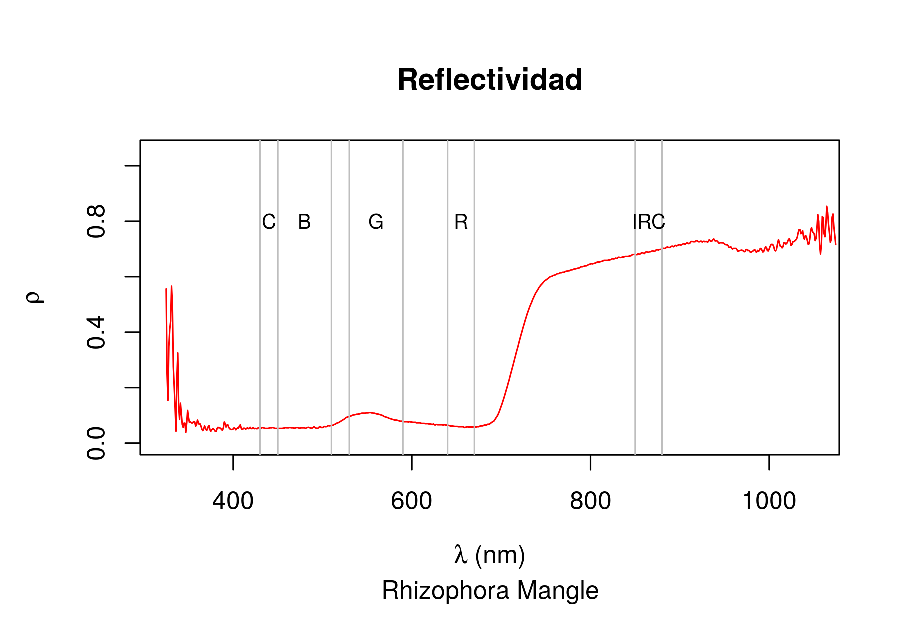
\includegraphics[width=0.8\linewidth]{./Imagenes/RM.eps}
%	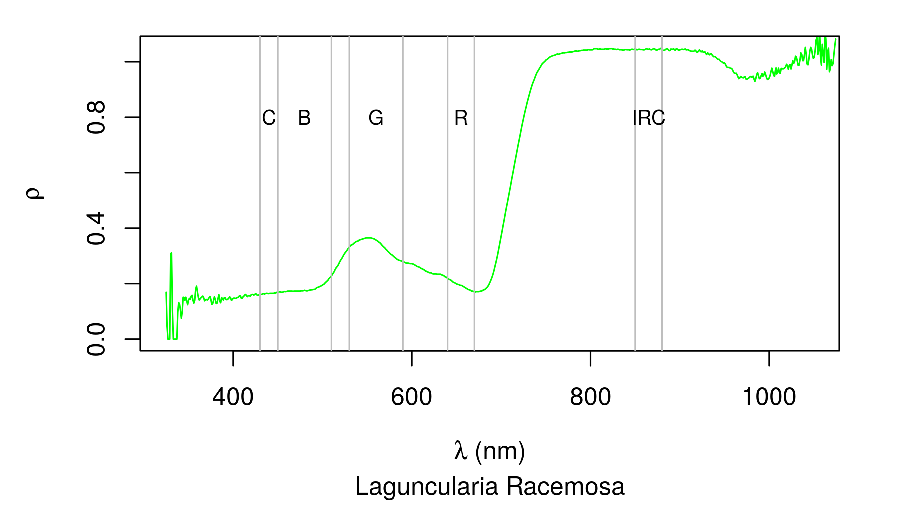
\includegraphics[width=0.8\linewidth]{./Imagenes/LR.eps}
%	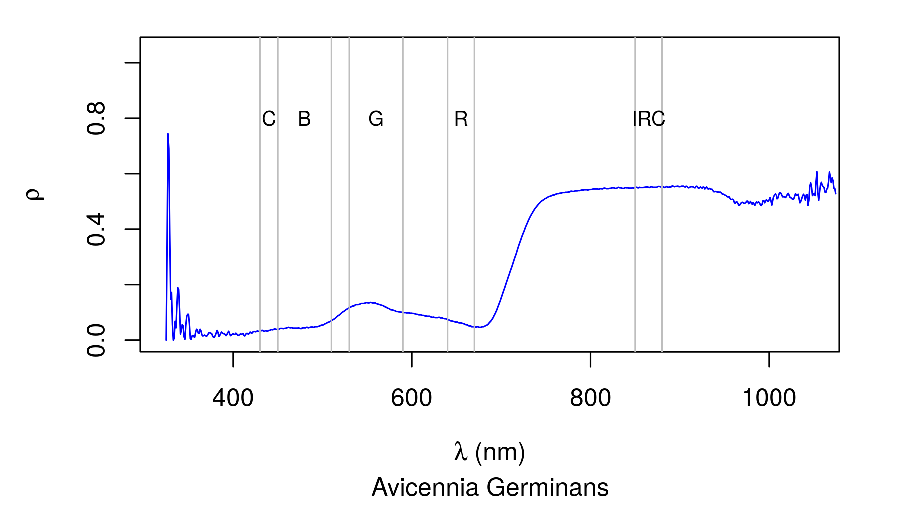
\includegraphics[width=0.8\linewidth]{./Imagenes/AG.eps}
%	\captionsetup{font={footnotesize,it}}
%	\caption[Firmas espectrales]{Gráficas de las firmas espectrales de las especies de mangle estudiadas. Fuente: Elaboración propia.}
%	\label{fig:firmas_espectrales}
%\end{figure}

\begin{figure}
	\centering
	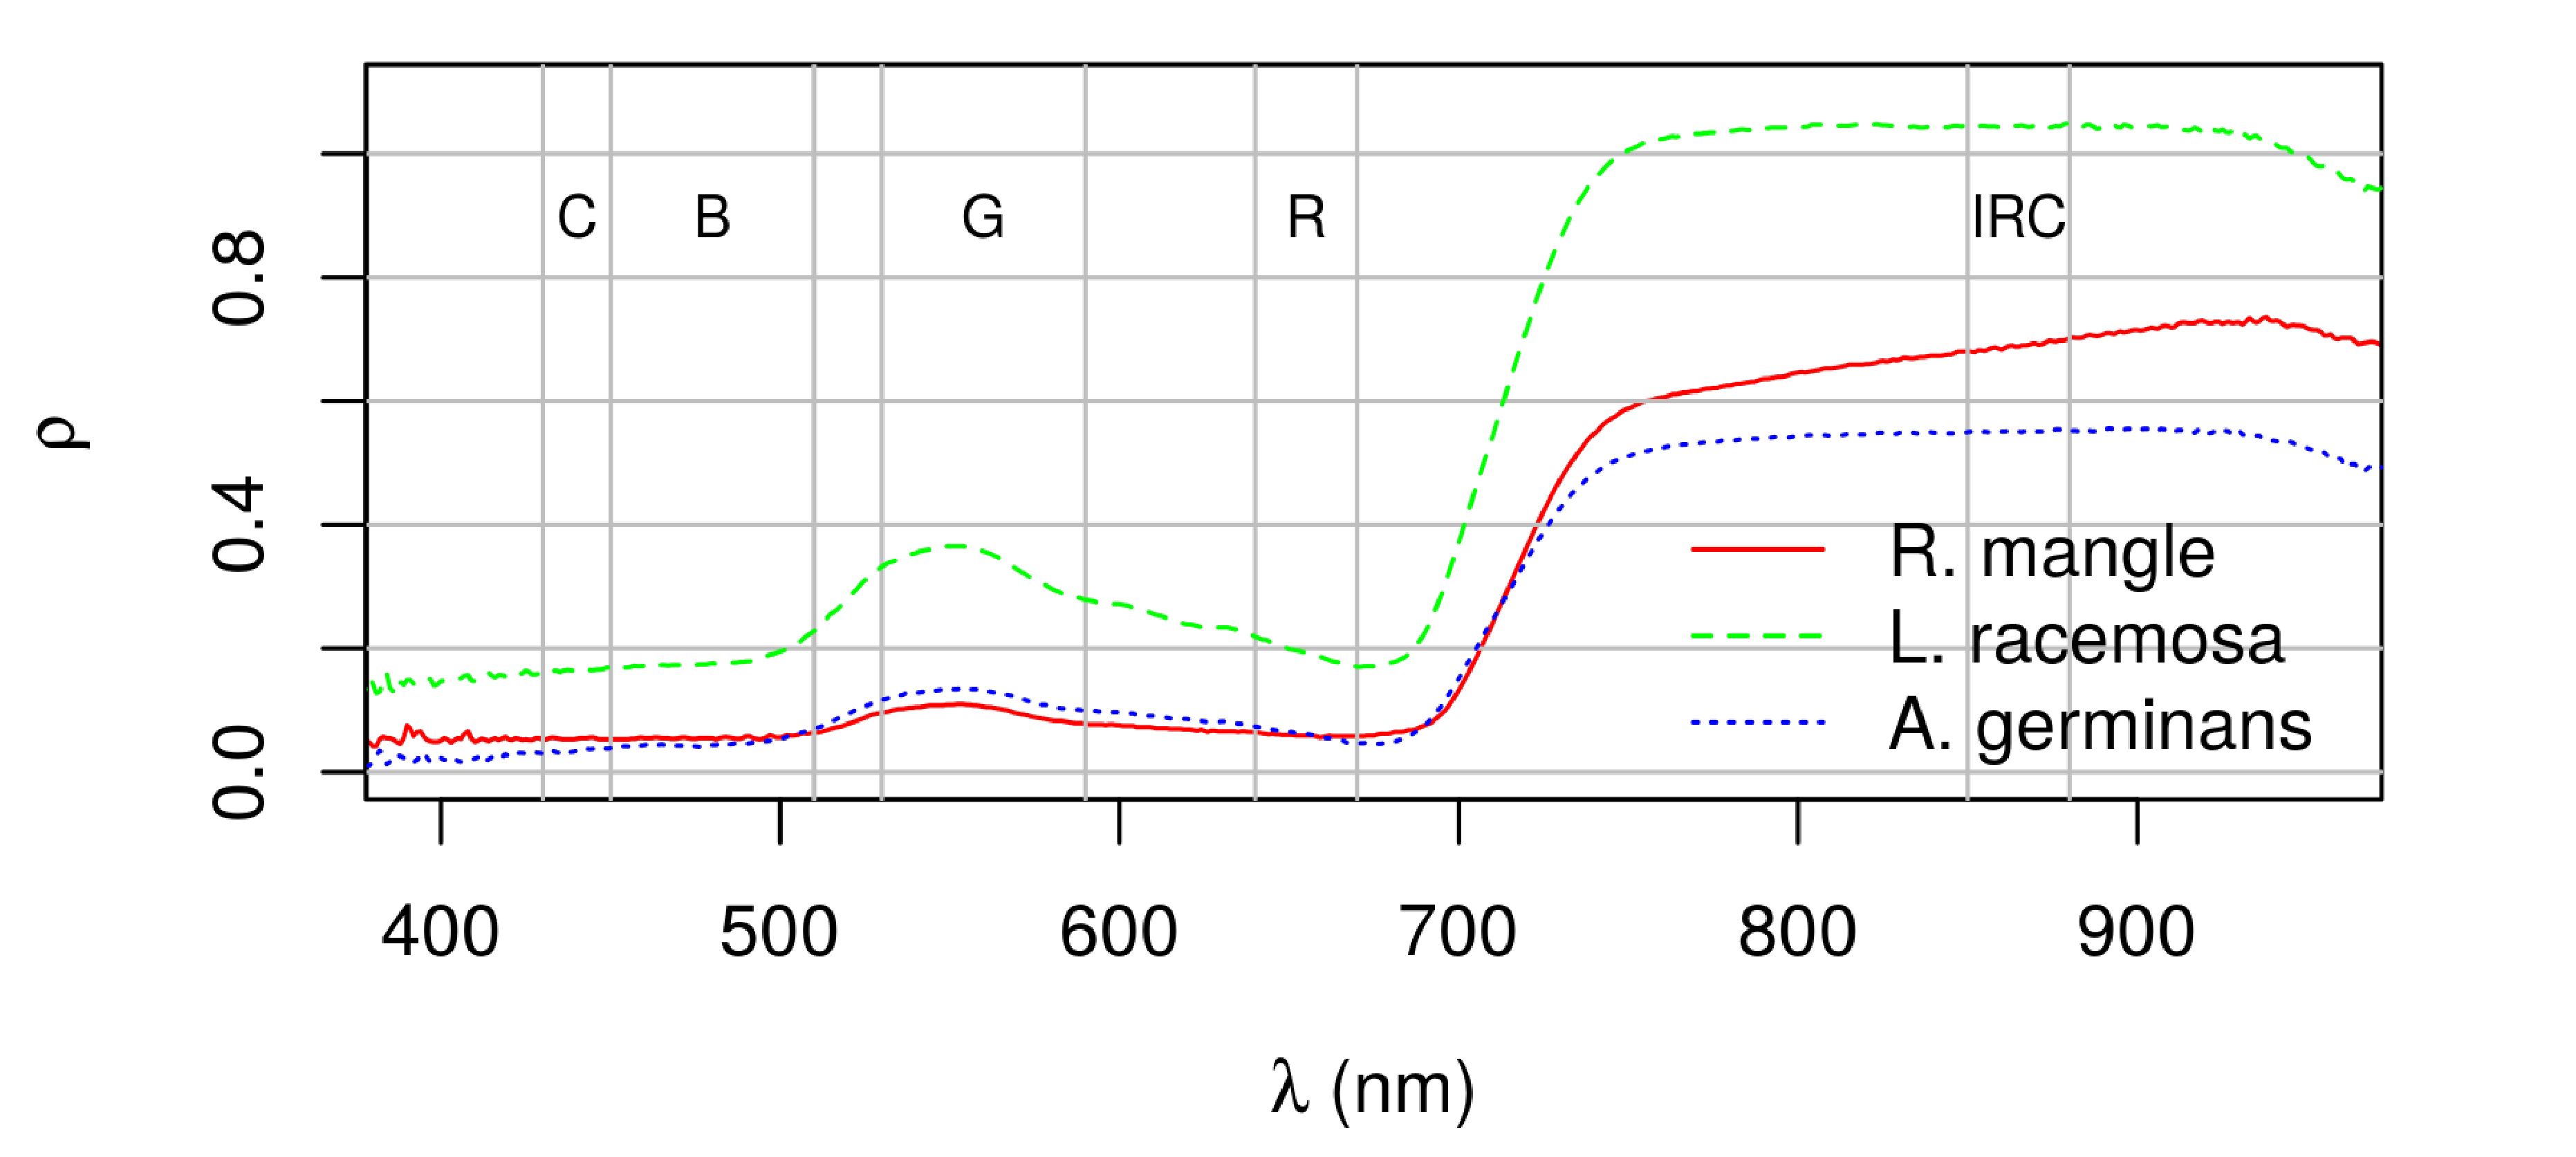
\includegraphics[width=0.8\linewidth]{./Imagenes/ral2.eps}
	\captionsetup{font={footnotesize,it}}
	\caption[Firmas espectrales de las tres especies]{Gráfica conjunta de las tres firmas espectrales. Elaboración propia.}
	\label{fig:ral}
\end{figure}

Como se aprecia, los datos presentan unas alteraciones al inicio y al final que son propias del radiómetro de campo. Se procedió a desechar estos datos haciendo un corte de colas entre los valores 420 nm y 900 nm de longitud de onda para preservar lo máximo posible la integridad de los datos y que no afectaran a los análisis de separabilidad. El número de observaciones se reduciría a 481 por las 751 originales. Las gráfica combinada resultante es la mostrada en la figura \ref{fig:ral_corte}.%\Sep

%\begin{figure}
%	\centering
%	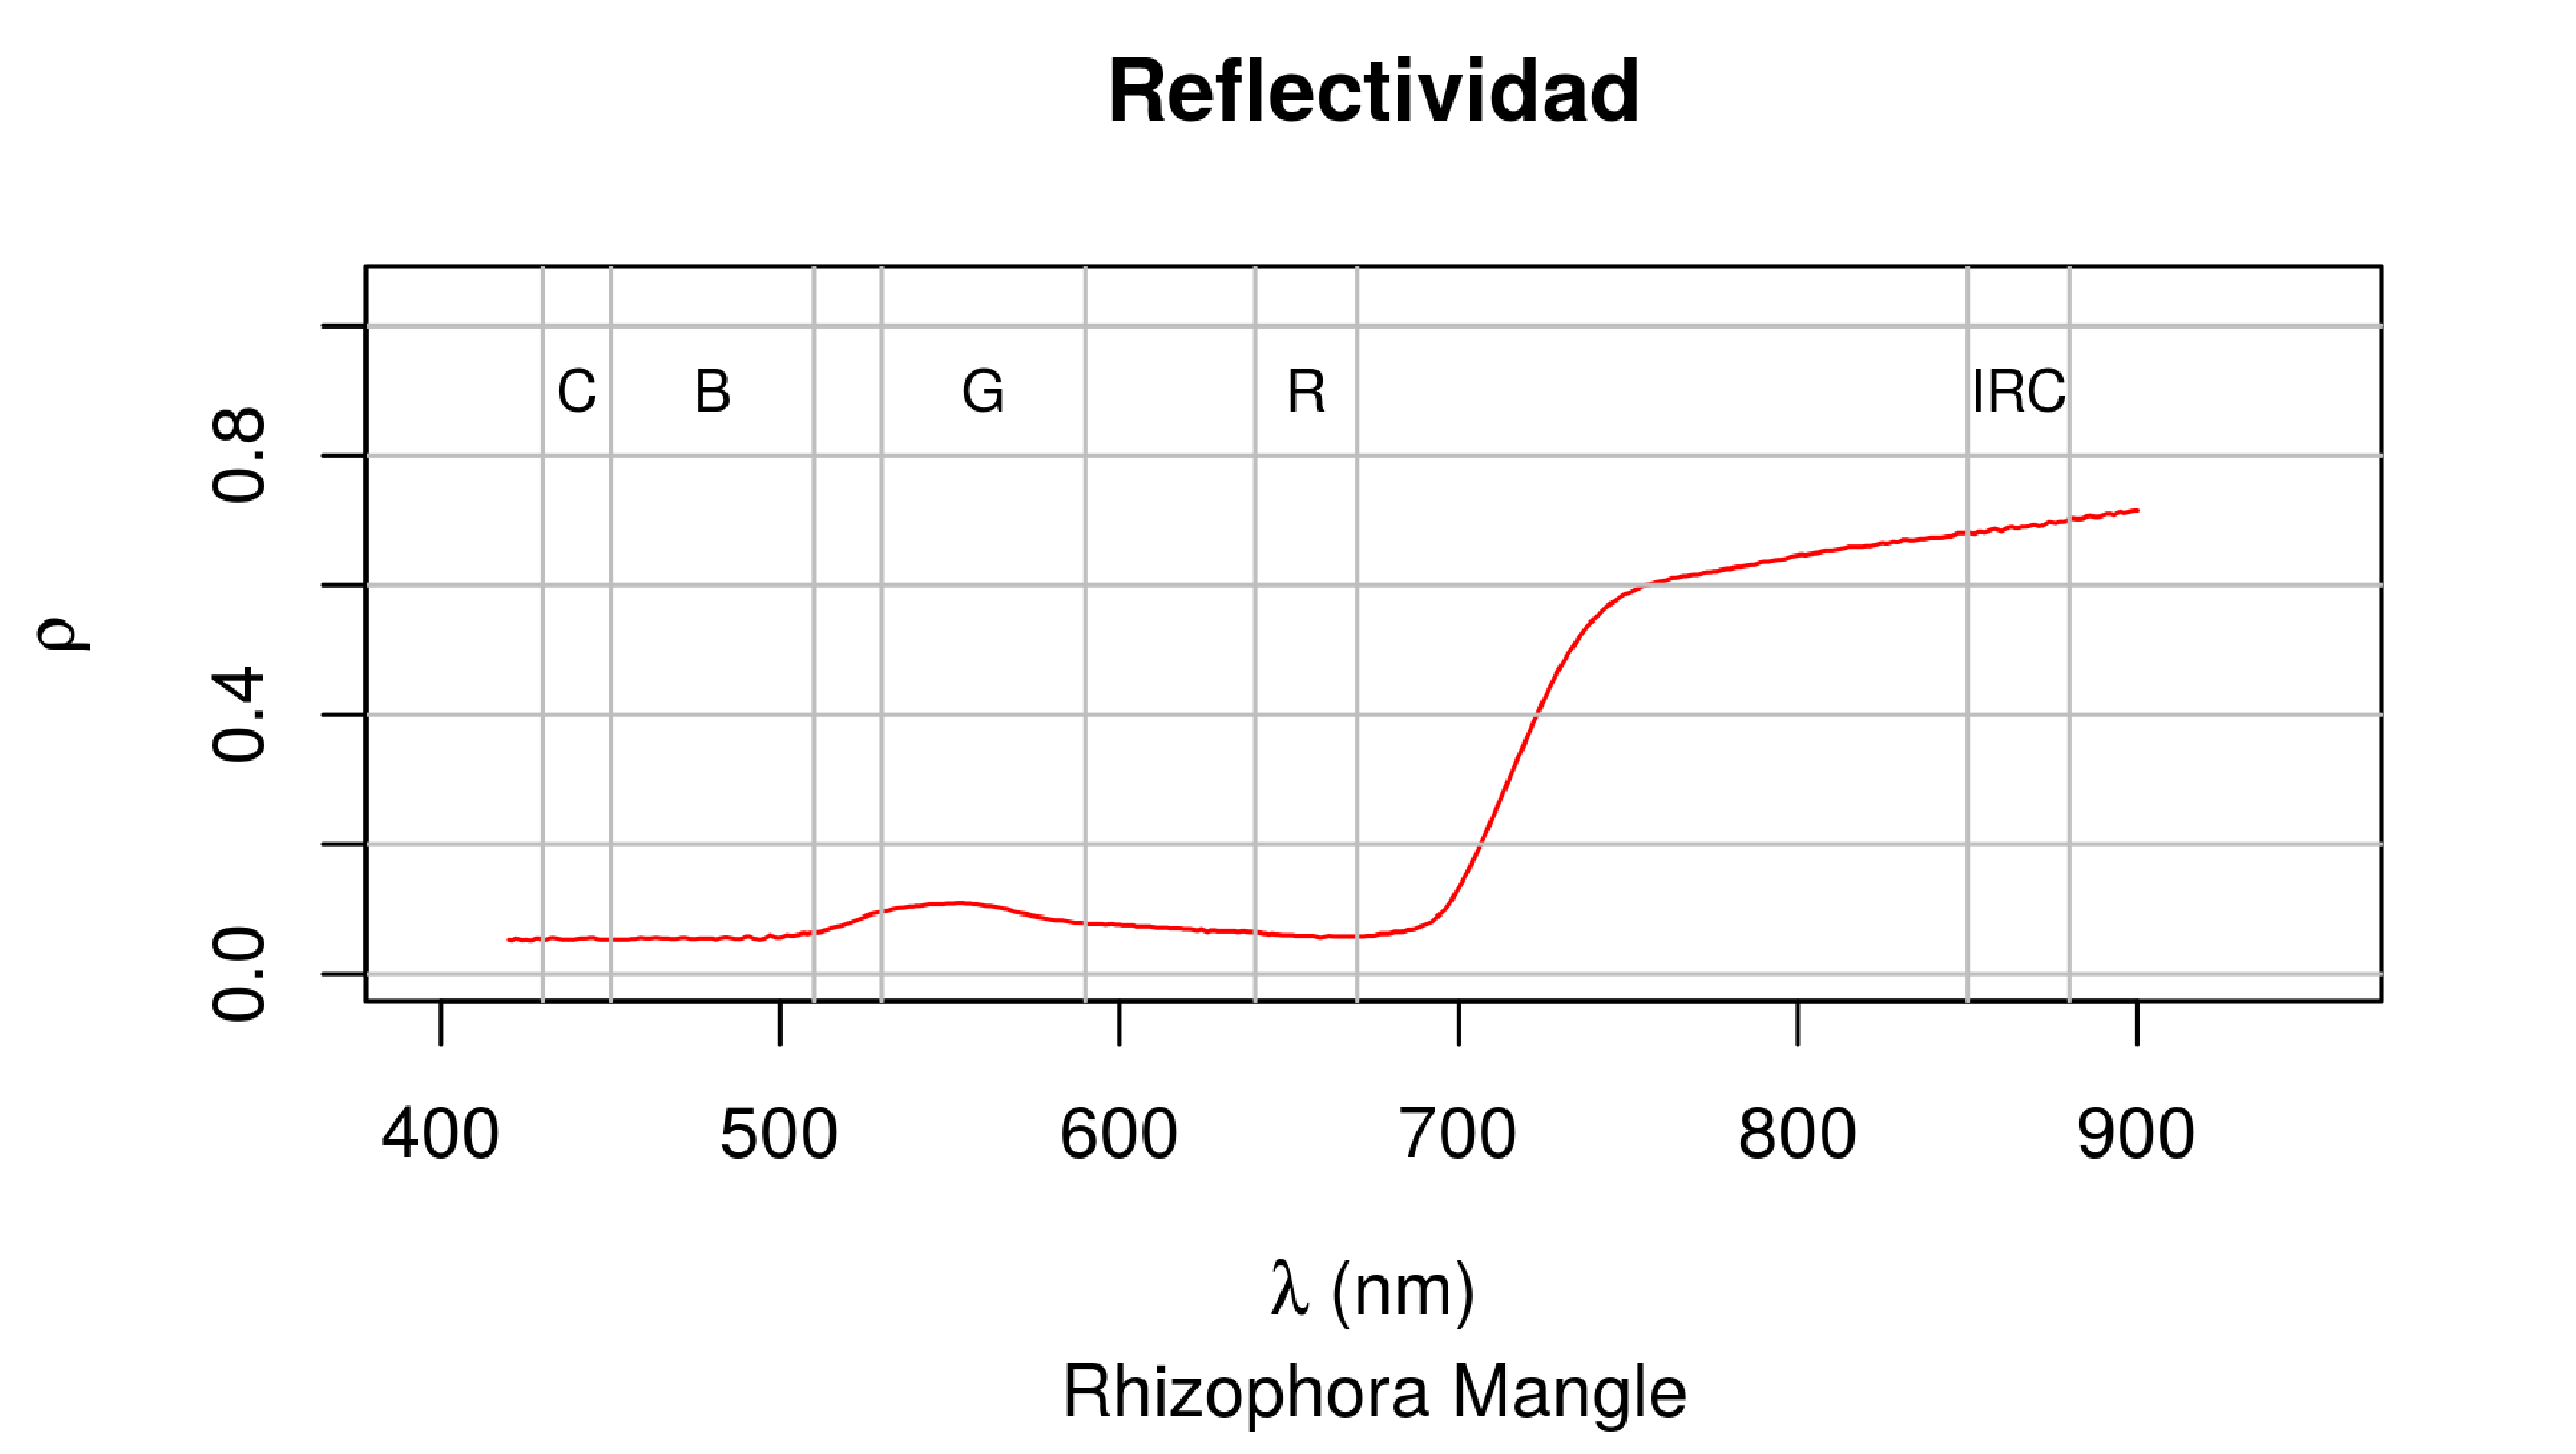
\includegraphics[width=0.8\linewidth]{./Imagenes/RMcorte.eps}
%	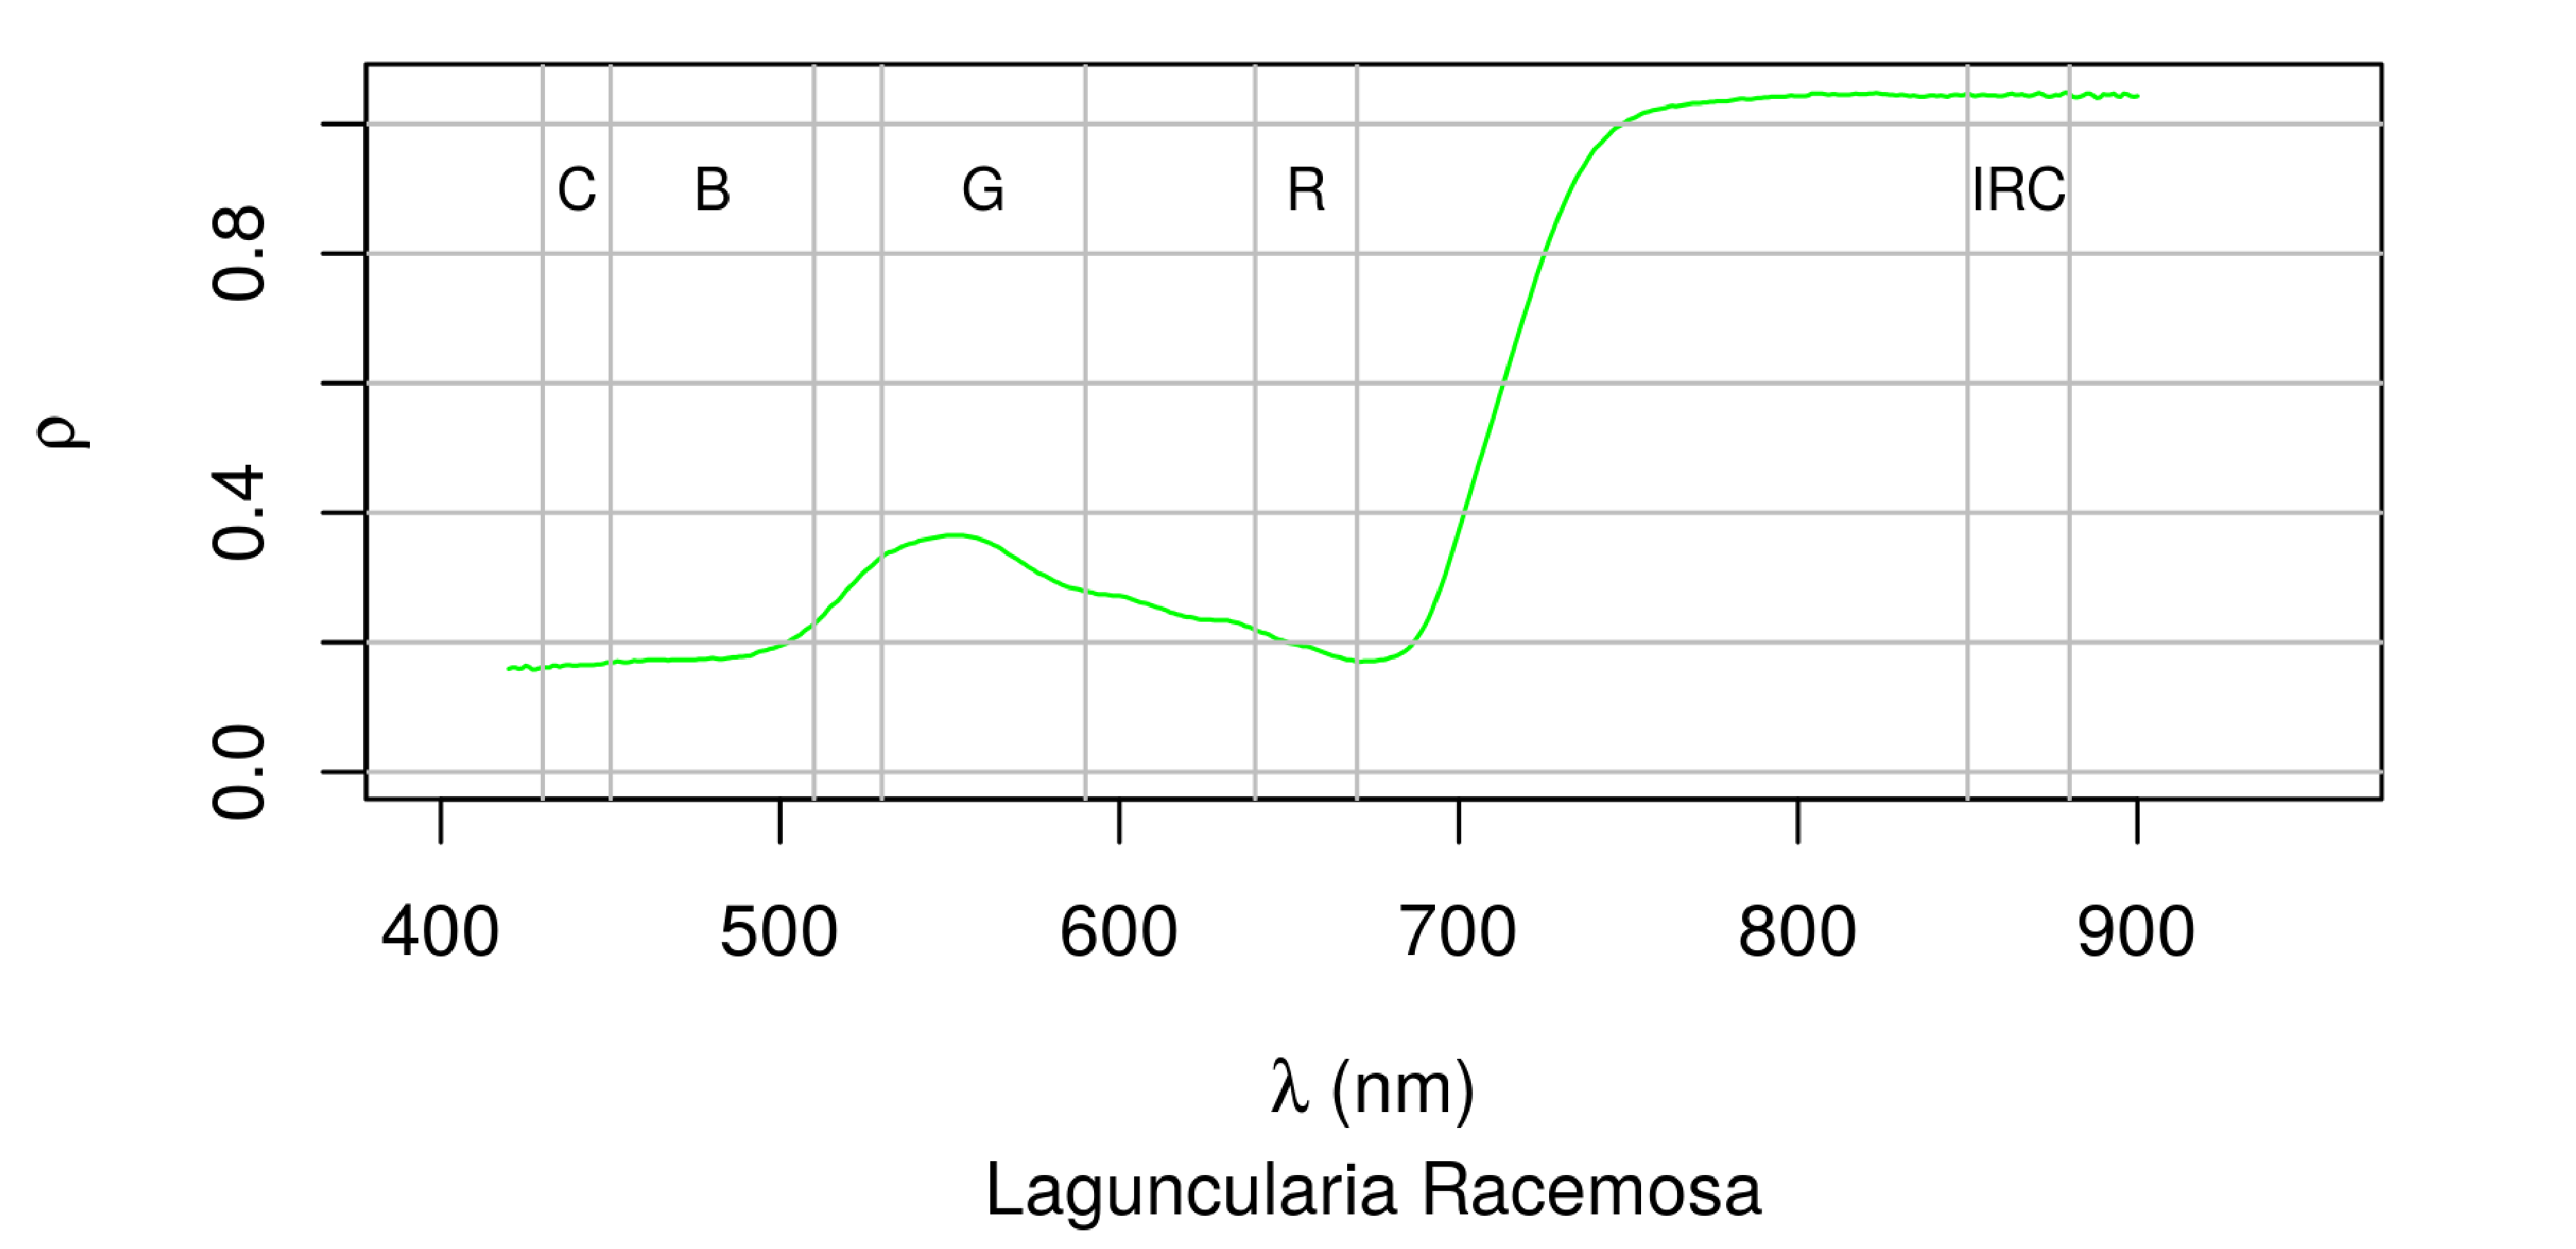
\includegraphics[width=0.8\linewidth]{./Imagenes/LRcorte.eps}
%	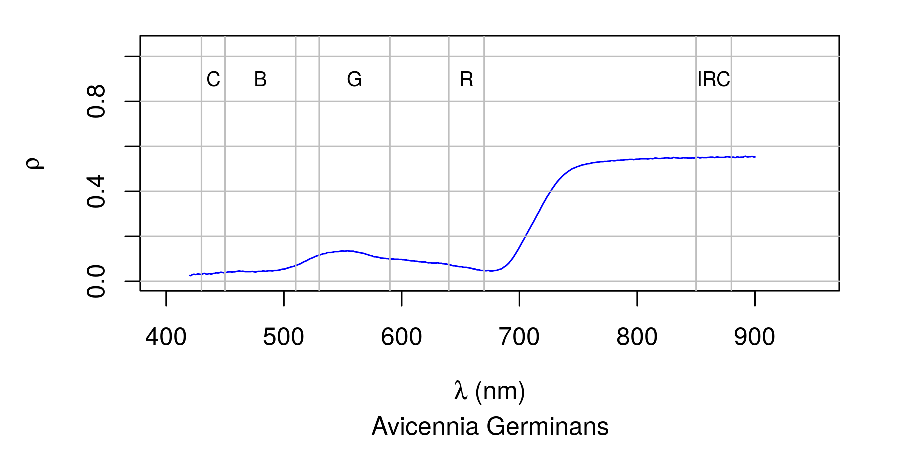
\includegraphics[width=0.8\linewidth]{./Imagenes/AGcorte.eps}
%	\captionsetup{font={footnotesize,it}}
%	\caption[Firmas espectrales cortadas]{Gráficas de las firmas espectrales de las especies de mangle estudiadas una vez realizado el corte de los datos. Elaboración propia.}
%	\label{fig:firmas_espectrales_corte}
%\end{figure}

\begin{figure}
	\centering
	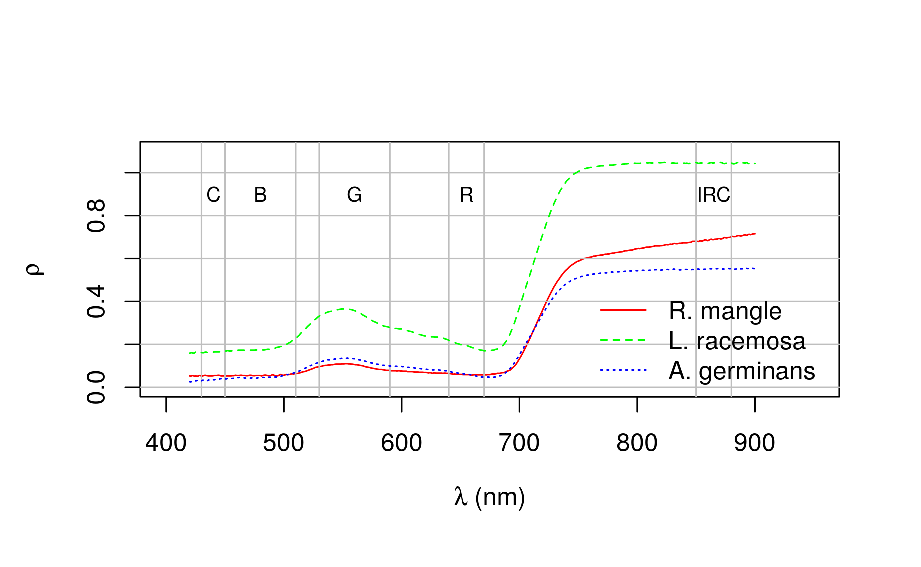
\includegraphics[width=0.8\linewidth]{./Imagenes/ralcorte.eps}
	\captionsetup{font={footnotesize,it}}
	\caption[Firmas espectrales cortadas de las tres especies]{Gráfica conjunta de las tres firmas espectrales una vez realizado el corte de los datos. Elaboración propia.}
	\label{fig:ral_corte}
\end{figure}

Las tres especies tienen un máximo local en la banda correspondiente al verde (G), típica de las especies vegetales, así como otro máximo de mayor valor, correspondientes al intervalo de longitud de onda ($\lambda$) en el que está incluida la banda del \ac{IRC}. Este último máximo también es característico de la vegetación e indicaría su grado de salud.%\Sep

Por lo tanto el primer vistazo a las gráficas es el esperado, siendo lo más preocupante el aparente parecido entre las especies R. mangle y A. germinans, que solo se diferencian en los valores del rango del \ac{IRC}.%\Sep

En el cuadro siguiente (\ref{tab:valores_medios}) se pueden apreciar los valores medios de cada especie para cada banda de Landsat 8.

\begin{table}[ht]
	\centering
	\begin{tabular}{@{}cccccc@{}}
	\toprule[0.4mm]
	Especie & Banda 1 (C) & Banda 2 (B) & Banda 3 (G) & Banda 4 (R) & Banda 5 (IRC) \\
	\midrule
	\textit{R. mangle}	& 0,0540 & 0,0561 & 0,0980 & 0,0595 & 0,6895 \\
	\textit{L. racemosa} & 0,1647 & 0,1821 & 0,3345 & 0,1930 & 1,0445 \\
	\textit{A. germinans} & 0,0355 & 0,0479 & 0,1218 & 0,0604 & 0,5513 \\
	\bottomrule[0.4mm]
	\end{tabular}
	\captionsetup{font={footnotesize,it}}
	\caption[Valores medios en las bandas Landsat]{Valores medios ara cada banda Landsat. Elaboración propia.}
	\label{tab:valores_medios}
\end{table}

\subsection{Índice de Acuerdo Espectral}
Una vez aplicando el script con la función de \ac{IAE} creado en R (figura \ref{fig:IAE}) ya se aprecia que el resultado no es muy bueno aunque esperado, siendo las diferencias casi inapreciables como se ve en la tabla \ref{tab:Valores_IAE}.%\Sep

\begin{table}[ht]
	\centering
	\begin{tabular}{@{}cccc@{}}
	\toprule
	& \textit{R. mangle} & \textit{L. racemosa} & \textit{A. germinans} \\
	\textit{R. mangle} & --- & 0,0083 & 0,0062 \\
	\textit{L. racemosa} & 0,0083 & --- & 0,0021 \\
	\textit{A. germinans} & 0,0062 & 0,0021 & --- \\
	\bottomrule[0.4mm]
	\end{tabular}
	\captionsetup{font={footnotesize,it}}
	\caption[Valores de IAE]{Valores de \ac{IAE} para cada par de especies de mangle. Elaboración propia.}
	\label{tab:Valores_IAE}
\end{table}

Las diferencias en este método son bajas debido a que se trata de tres especies que, aunque no sean de la misma familia, si son vegetales y coexisten formando asociación en el mismo ecosistema. De haber estudiado la diferencia entre especie vegetal, suelo y agua por ejemplo, las diferencias habrían sido más notables debido a la diferencia de valor medio de la respuesta espectral. En este caso, el valor medio de las tres especies sería el mostrado en el cuadro \ref{tab:mediaIAE}. El corte en $\lambda$ que se menciona en el cuadro se refiere al valor de longitud de onda a partir del cual la reflectancia es mayor a la media y por tanto se provoca una cambio en el valor binario de 0 a 1 donde, de tener un mayor rango de longitud de onda observada habría más de un cambio. Se observan unos valores similares de $\lambda$ para las tres especies, pero donde sí se notan diferencias son en el valor medio de la reflectancia, siendo el de la \textit{L. racemosa} notablemente superior al de las otras dos especies.%\Sep

\begin{table}
	\centering
	\begin{tabular}{@{}ccc@{}}
	\toprule[0.4mm]
	Especie & $\rho$ media & Corte en $\lambda$ (nm)\\
	\midrule
	\textit{R. mangle} & 0,2897692 & 714	\\
	\textit{L. racemosa} & 0,5424927 & 710\\
	\textit{A. germinans} & 0,2530166 & 711\\
	\bottomrule
	\end{tabular}
	\captionsetup{font={footnotesize,it}}
	\caption[Valores medios de la respuesta espectral]{Valor medio de la respuesta espectral para cada especie. Elaboración propia.}
	\label{tab:mediaIAE}
\end{table}

%\begin{figure}
%	\centering
%	\includegraphics[width=0.8\linewidth]{./Imagenes/IAE_RM.eps}
%	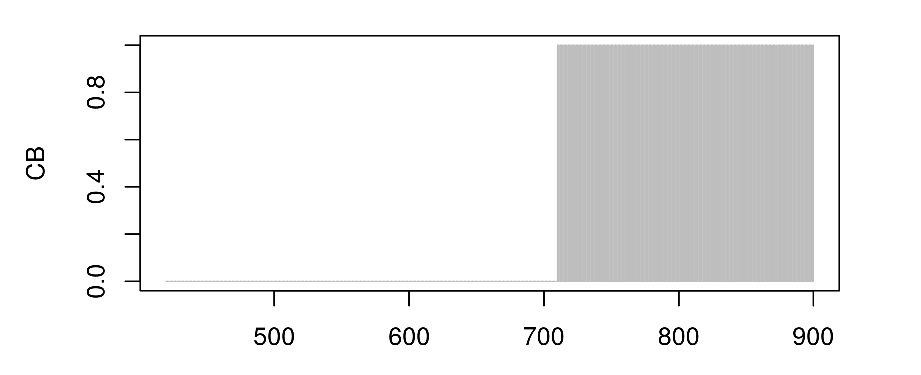
\includegraphics[width=0.8\linewidth]{./Imagenes/IAE_LR.eps}
%	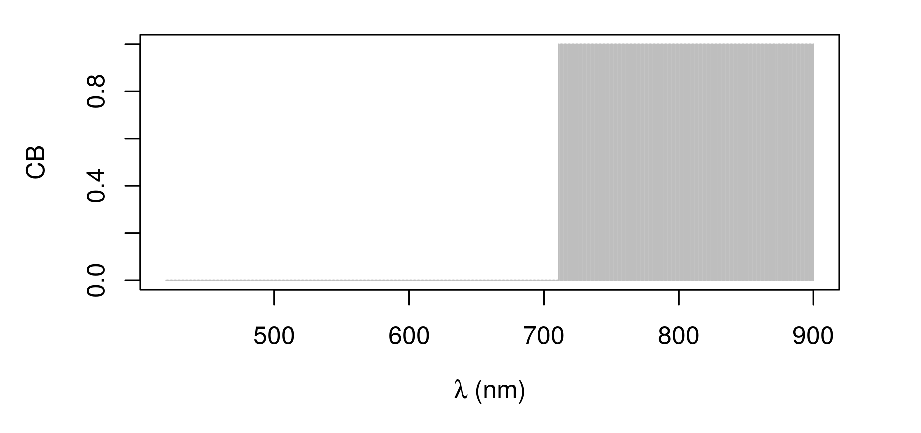
\includegraphics[width=0.8\linewidth]{./Imagenes/IAE_AG.eps}
%	\captionsetup{font={footnotesize,it}}
%	\caption[Gráficas de combinación binaria]{Gráficas de combinación binaria de las tres especies de mangle, por orden \textit{Rhizophora mangle}, \textit{Laguncularia racemosa} y \textit{Avicennia germinans}. Elaboración propia.}
%	\label{fig:CB}
%\end{figure}

\subsection{\textit{Continuum Removal}}
En la gráfica de la figura \ref{fig:GraficaCR} se pueden observar las diferencias entre las tres especies que nos indica este tipo de análisis. Son tres los aspectos de esta gráfica a analizar: la profundidad y anchura de las partes convexas y la posición de los puntos mínimos. En gris la gráfica de reflectividad de cada especie.%\Sep

\begin{figure}
	\centering
	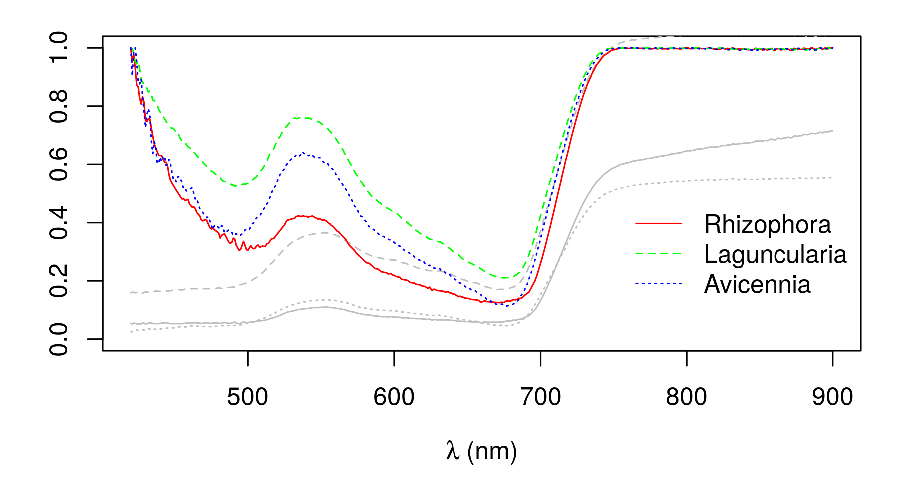
\includegraphics[width=0.8\linewidth]{./Imagenes/ContinuumR2.eps}
	\captionsetup{font={footnotesize,it}}
	\caption[Gráfica de \textit{Continuum Removal}]{Gráfica de \textit{Continuum Removal} para las tres especies de mangle. Elaboración propia.}
	\label{fig:GraficaCR}
\end{figure}

En cuanto a la profundidad se observa una clara absorción en torno a los 490 nm y los 680 nm de las tres especies. En el caso de la \textit{A. germinans} esta absorción es más acusada en ambos puntos. \textit{R. mangle} y \textit{L. racemosa} muestran un comportamiento similar en la primera zona mientras que en la segunda la \textit{L. racemosa} no muestra la absorción de la \textit{R. mangle}.%\Sep

En cuanto a la anchura lo más llamativo es la amplitud de los valores de la \textit{R. mangle} en torno a los valores centrales de la observación.

\subsection{Clasificación angular}
Una vez aplicado el script de R de la función de clasificación angular (figura \ref{fig:AE}), los valores son los de la siguiente tabla:

\begin{table}[ht]
	\centering	
	\begin{tabular}{@{}cccc@{}}
	\toprule[0.4mm]
	& \textit{R. mangle} & \textit{L. racemosa} & \textit{A. germinans} \\
	\textit{R. mangle} & --- & 0,1651 (9,5401) & 0,0752 (4,3086) \\
	\textit{L. racemosa} & 0,1651 (9,5401) & --- & 0,1062 (6,0826) \\
	\textit{A. germinans} & 0,0752 (4,3086) & 0,1062 (6,0826) & --- \\
	\bottomrule[0.4mm]
	\end{tabular}
	\captionsetup{font={footnotesize,it}}
	\caption[Valores de Ángulo Espectral]{Valores del Ángulo Espectral en radianes. Ángulo sexagesimal entre paréntesis. Elaboración propia.}	
\end{table}

Se puede observar una mayor separabilidad entre \textit{R. mangle} y \textit{L. racemosa}, siendo menor en las otras combinaciones.

\section{Combinación de bandas}
Para observar las zonas donde hay presencia de bosque de mangle basta con realizar diversas combinaciones de bandas de Landsat 8. A las figuras ya expuestas en el capítulo de materiales y métodos (figuras \ref{fig:gf432} y \ref{fig:gf543}) correspondientes al color real y a un falso color con realce del \ac{IRC} en el canal rojo. En las figuras \ref{fig:gf654} y \ref{fig:gf562} se muestran combinaciones que también buscan conseguir un realce del manglar. Por las propiedades de reflectividad de la cubierta combinando bandas del infrarrojo se obtienen buenos resultados para realizar un análisis visual.

\begin{figure}
	\centering
	\includegraphics[width=0.8\linewidth]{./Imagenes/GF654.eps}
	\captionsetup{font={footnotesize,it}}
	\caption[Composición 654]{Resultado de la imagen en una composición de realce de vegetación (6-5-4). Imagen exportada de GRASS. Elaboración propia.}
	\label{fig:gf654}
\end{figure}

\begin{figure}
	\centering
	\includegraphics[width=0.8\linewidth]{./Imagenes/GF562.eps}
	\captionsetup{font={footnotesize,it}}
	\caption[Composición 562]{Resultado de la imagen en una composición de realce de vegetación (5-6-2). Imagen exportada de GRASS. Elaboración propia.}
	\label{fig:gf562}
\end{figure}

\section{Comprobación}
Debido a que en la corrección utilizada en las imágenes \ac{PL8SR} los valores vienen presentados con un factor de escala de 0,0001 \citep{USGS2015} corresponde reescalar los valores a un intervalo 0-1 más común. Para ello se emplea la calculadora de mapas ráster de GRASS aplicando la expresión $L8GF\_SRFB1@TFG \cdot 0.0001$ para cada una de las capas del proyecto. La línea de comando utilizada es la siguiente:

\begin{figure}[ht]
	\centering
	\begin{boxedverbatim}
	r.mapcalc `L8GF_B1=L8GF_SRFB1@TFG*0.0001'
	\end{boxedverbatim}
	\captionsetup{font={footnotesize,it}}
	\caption[Reescalado de valores]{Reescalado de los valores de la imagen Landsat con r.mapcalc.}
\end{figure}

Se muestran los valores resultantes para cada punto en el cuadro \ref{tab:tabla_puntos} y su distribución en la zona de estudio en la figura \ref{fig:dist_puntos}.%\Sep

\begin{table}[ht]
	\centering
	\begin{tabular}{@{}cccccccc@{}}
	\toprule[0.4mm]
	cat & x & y & B1 & B2 & B3 & B4 & B5\\
	\midrule
	1 & 413076,12 & 1485451,42 & 0,0080 & 0,0102 & 0,0249 & 0,0120 & 0,3054\\
	2 & 416539,92 & 1483130,35 & 0,0096 & 0,0113 & 0,0254 & 0,0137 & 0,2964\\
	3 & 413619,63 & 1482194,38 & 0,0090 & 0,0108 & 0,0247 & 0,0116 & 0,3311\\
	4 & 434978,06 & 1485551,73 & 0,0076 & 0,0099 & 0,0256 & 0,0124 & 0,3132\\
	5 & 435666,27 & 1481906,87 & 0,0086 & 0,0109 & 0,0254 & 0,0134 & 0,2954\\
	6 & 426223,06 & 1479693,58 & 0,0106 & 0,0131 & 0,0330 & 0,0173 & 0,2963\\
	7 & 434938,70 & 1478948,70 & 0,0119 & 0,0146 & 0,0309 & 0,0190 & 0,2612\\
	8 & 455289,36 & 1479452,68 & 0,0132 & 0,0163 & 0,0385 & 0,0268 & 0,2300\\
	9 & 447490,46 & 1478621,82 & 0,0147 & 0,0187 & 0,0413 & 0,0286 & 0,2300\\
	10 & 452584,20 & 1462969,61 & 0,0115 & 0,0143 & 0,0345 & 0,0209 & 0,2577\\
	\bottomrule[0.4mm]
	\end{tabular}
	\captionsetup{font={footnotesize,it}}
	\caption[Base de datos de puntos de comprobación]{Base de datos asociada a la capa vectorial ``puntos'' de la figura \ref{fig:dist_puntos}. Elaboración propia.}
	\label{tab:tabla_puntos}
\end{table}

\begin{figure}
	\centering
	\includegraphics[width=0.8\linewidth]{./Imagenes/puntos_comprob.eps}
	\captionsetup{font={footnotesize,it}}
	\caption[Distribución de puntos]{Distribución de puntos de comprobación en la zona de estudio. Elaboración propia.}
	\label{fig:dist_puntos}
\end{figure}

Para hacer una comprobación de los datos tomados en campo se superponen estos a una gráfica de cajas y bigotes extraída de los valores de los puntos de comprobación (figura \ref{fig:grafica_comprob}). Un gráfico de este tipo consiste en una caja rectangular donde los lados verticales (en nuestro caso) muestran el recorrido intercuartílico dividido por un segmento horizontal que es la mediana. Por lo tanto, de un solo vistazo nos aporta información sobre valor central (segunto cuartil), primer y tercer cuartil. Además nos dice cuales son los valores máximo y mínimo de la distribución, que formarían los bigotes, y detecta valores desfasados en forma de puntos fuera de la caja.%\Sep

Gracias a esta representación gráfica se confirma que la magnitud de los datos tomados por el espectro-radiómetro de campo están incrementados en varias décimas en la lectura media de cada banda comparados con la información de las imágenes de Landsat 8. Pese a eso se puede observar como los datos tienen un aspecto similar.

\begin{figure}
	\centering
	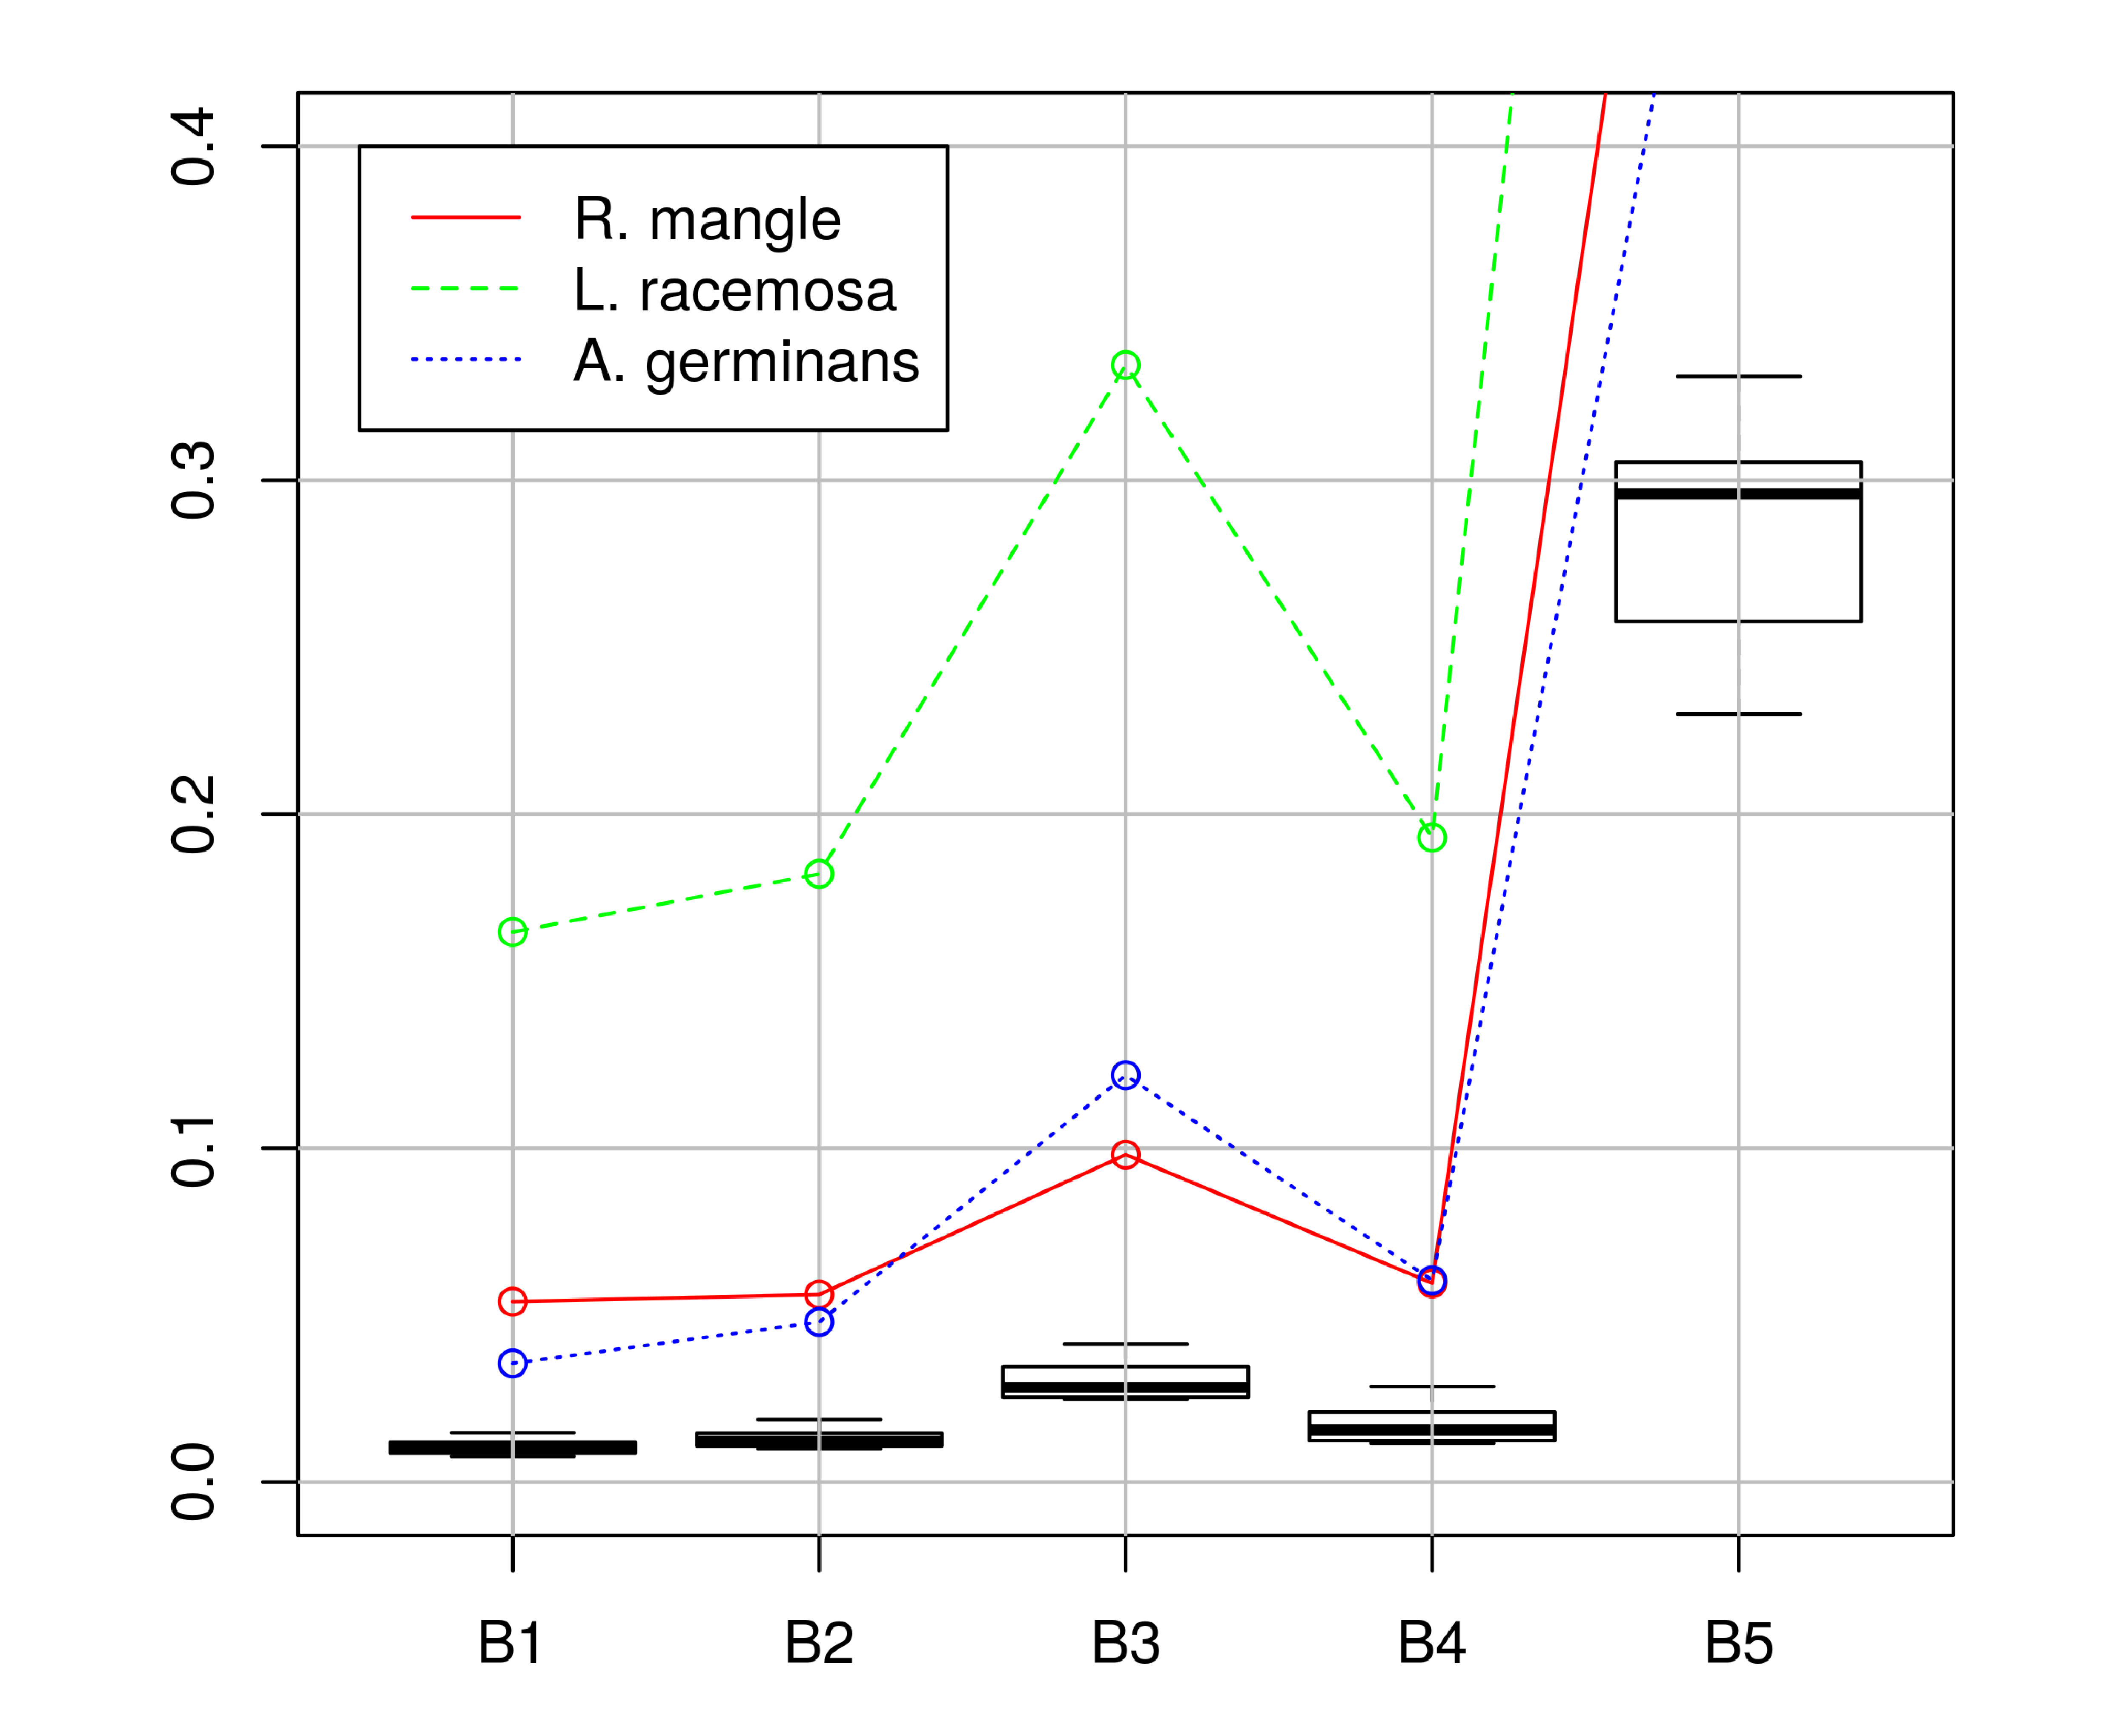
\includegraphics[width=0.8\linewidth]{./Imagenes/grafica_comprob.eps}
	\captionsetup{font={footnotesize,it}}
	\caption[Gráfico de puntos de comprobación]{Gráfico de cajas y bigotes correspondiente a los datos de los puntos de comprobación. Se superponen los datos medios de reflectividad para cada especie en cada banda. Elaboración propia.}
	\label{fig:grafica_comprob}
\end{figure}


\section{Clasificación de imágenes}
En las clasificaciones se muestra confusión de clases, mezclándose en algunos casos el mangle con otro tipo de vegetación en zonas donde, por las propias características del ecosistema, es imposible la existencia de manglar (detalle en \ref{fig:detalle_clasnosup}). A excepción de la clasificación supervisada que, a pesar de que se ve un exceso de la clase denominada ``Agua 2'' en zonas donde no hay presencia de esta, discrimina bien la cobertura de mangle de otros tipos (detalle en figura \ref{fig:detalle_classup}).%\Sep

\begin{figure}
	\centering
	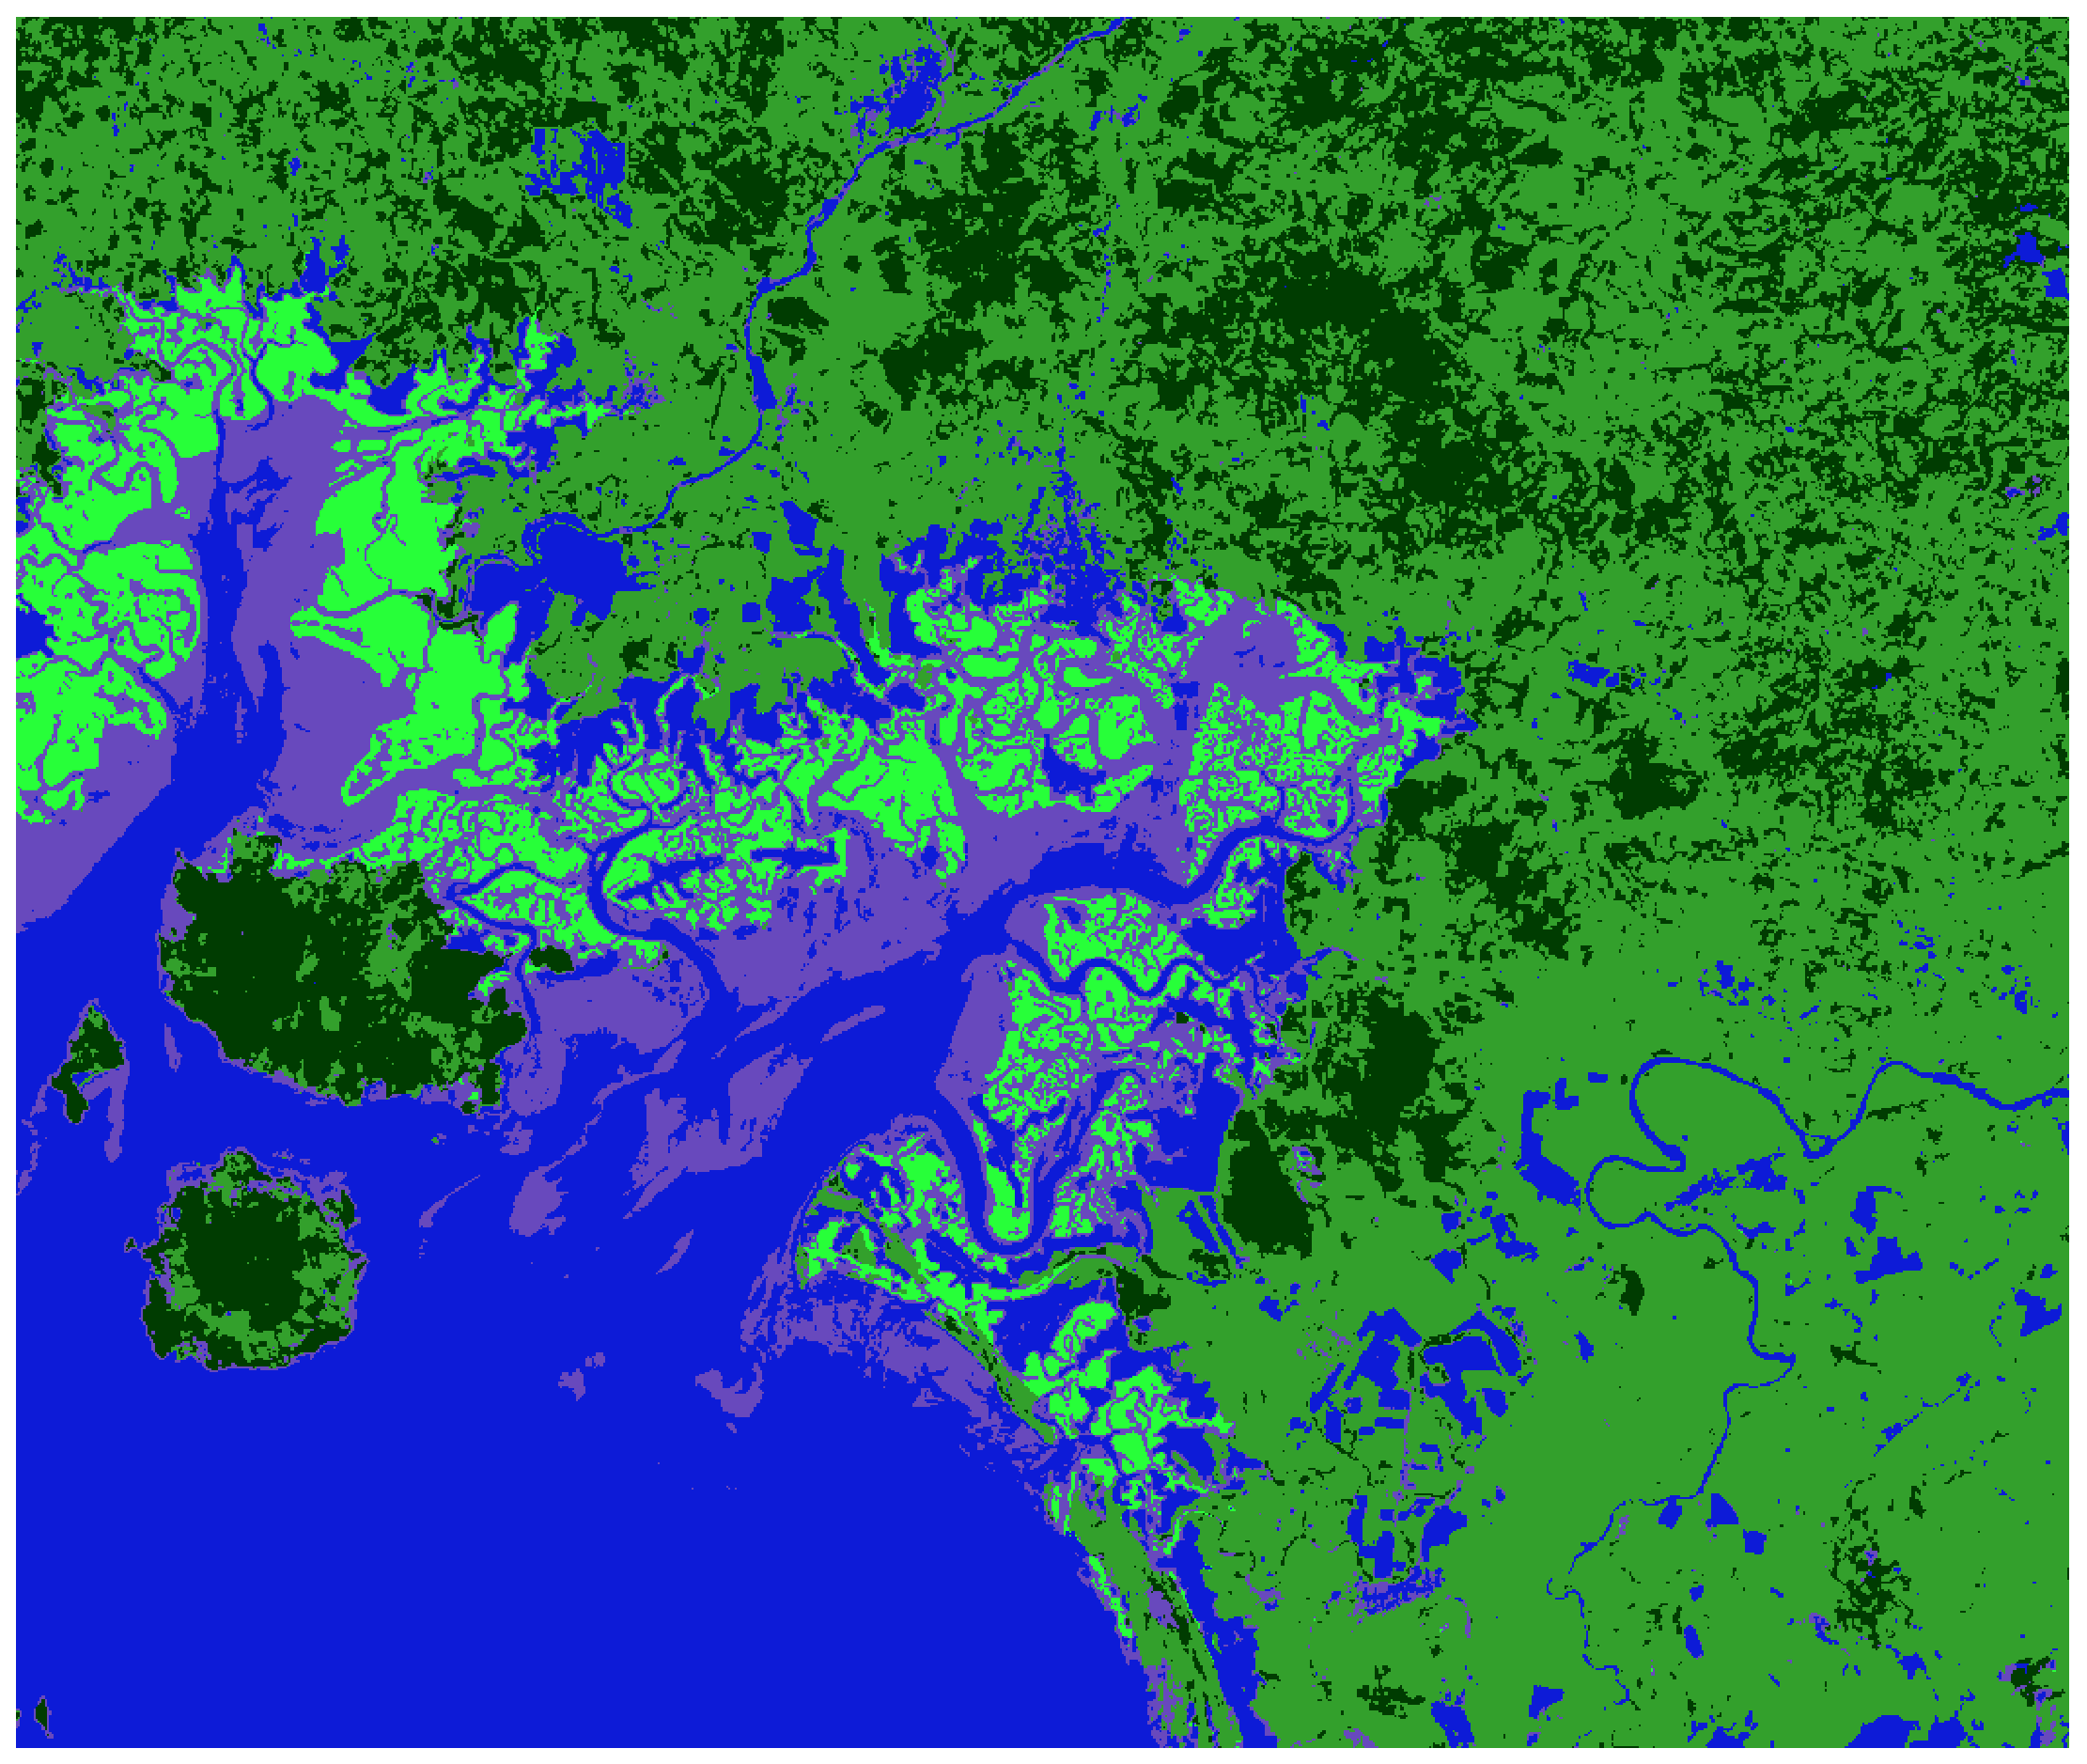
\includegraphics[width=0.8\linewidth]{./Imagenes/Detalle_classup.eps}
	\captionsetup{font={footnotesize,it}}
	\caption[Detalle clasificación supervisada]{Detalle de la clasificación supervisada. Elaboración propia.}
	\label{fig:detalle_classup}
\end{figure}

\begin{figure}
	\centering
	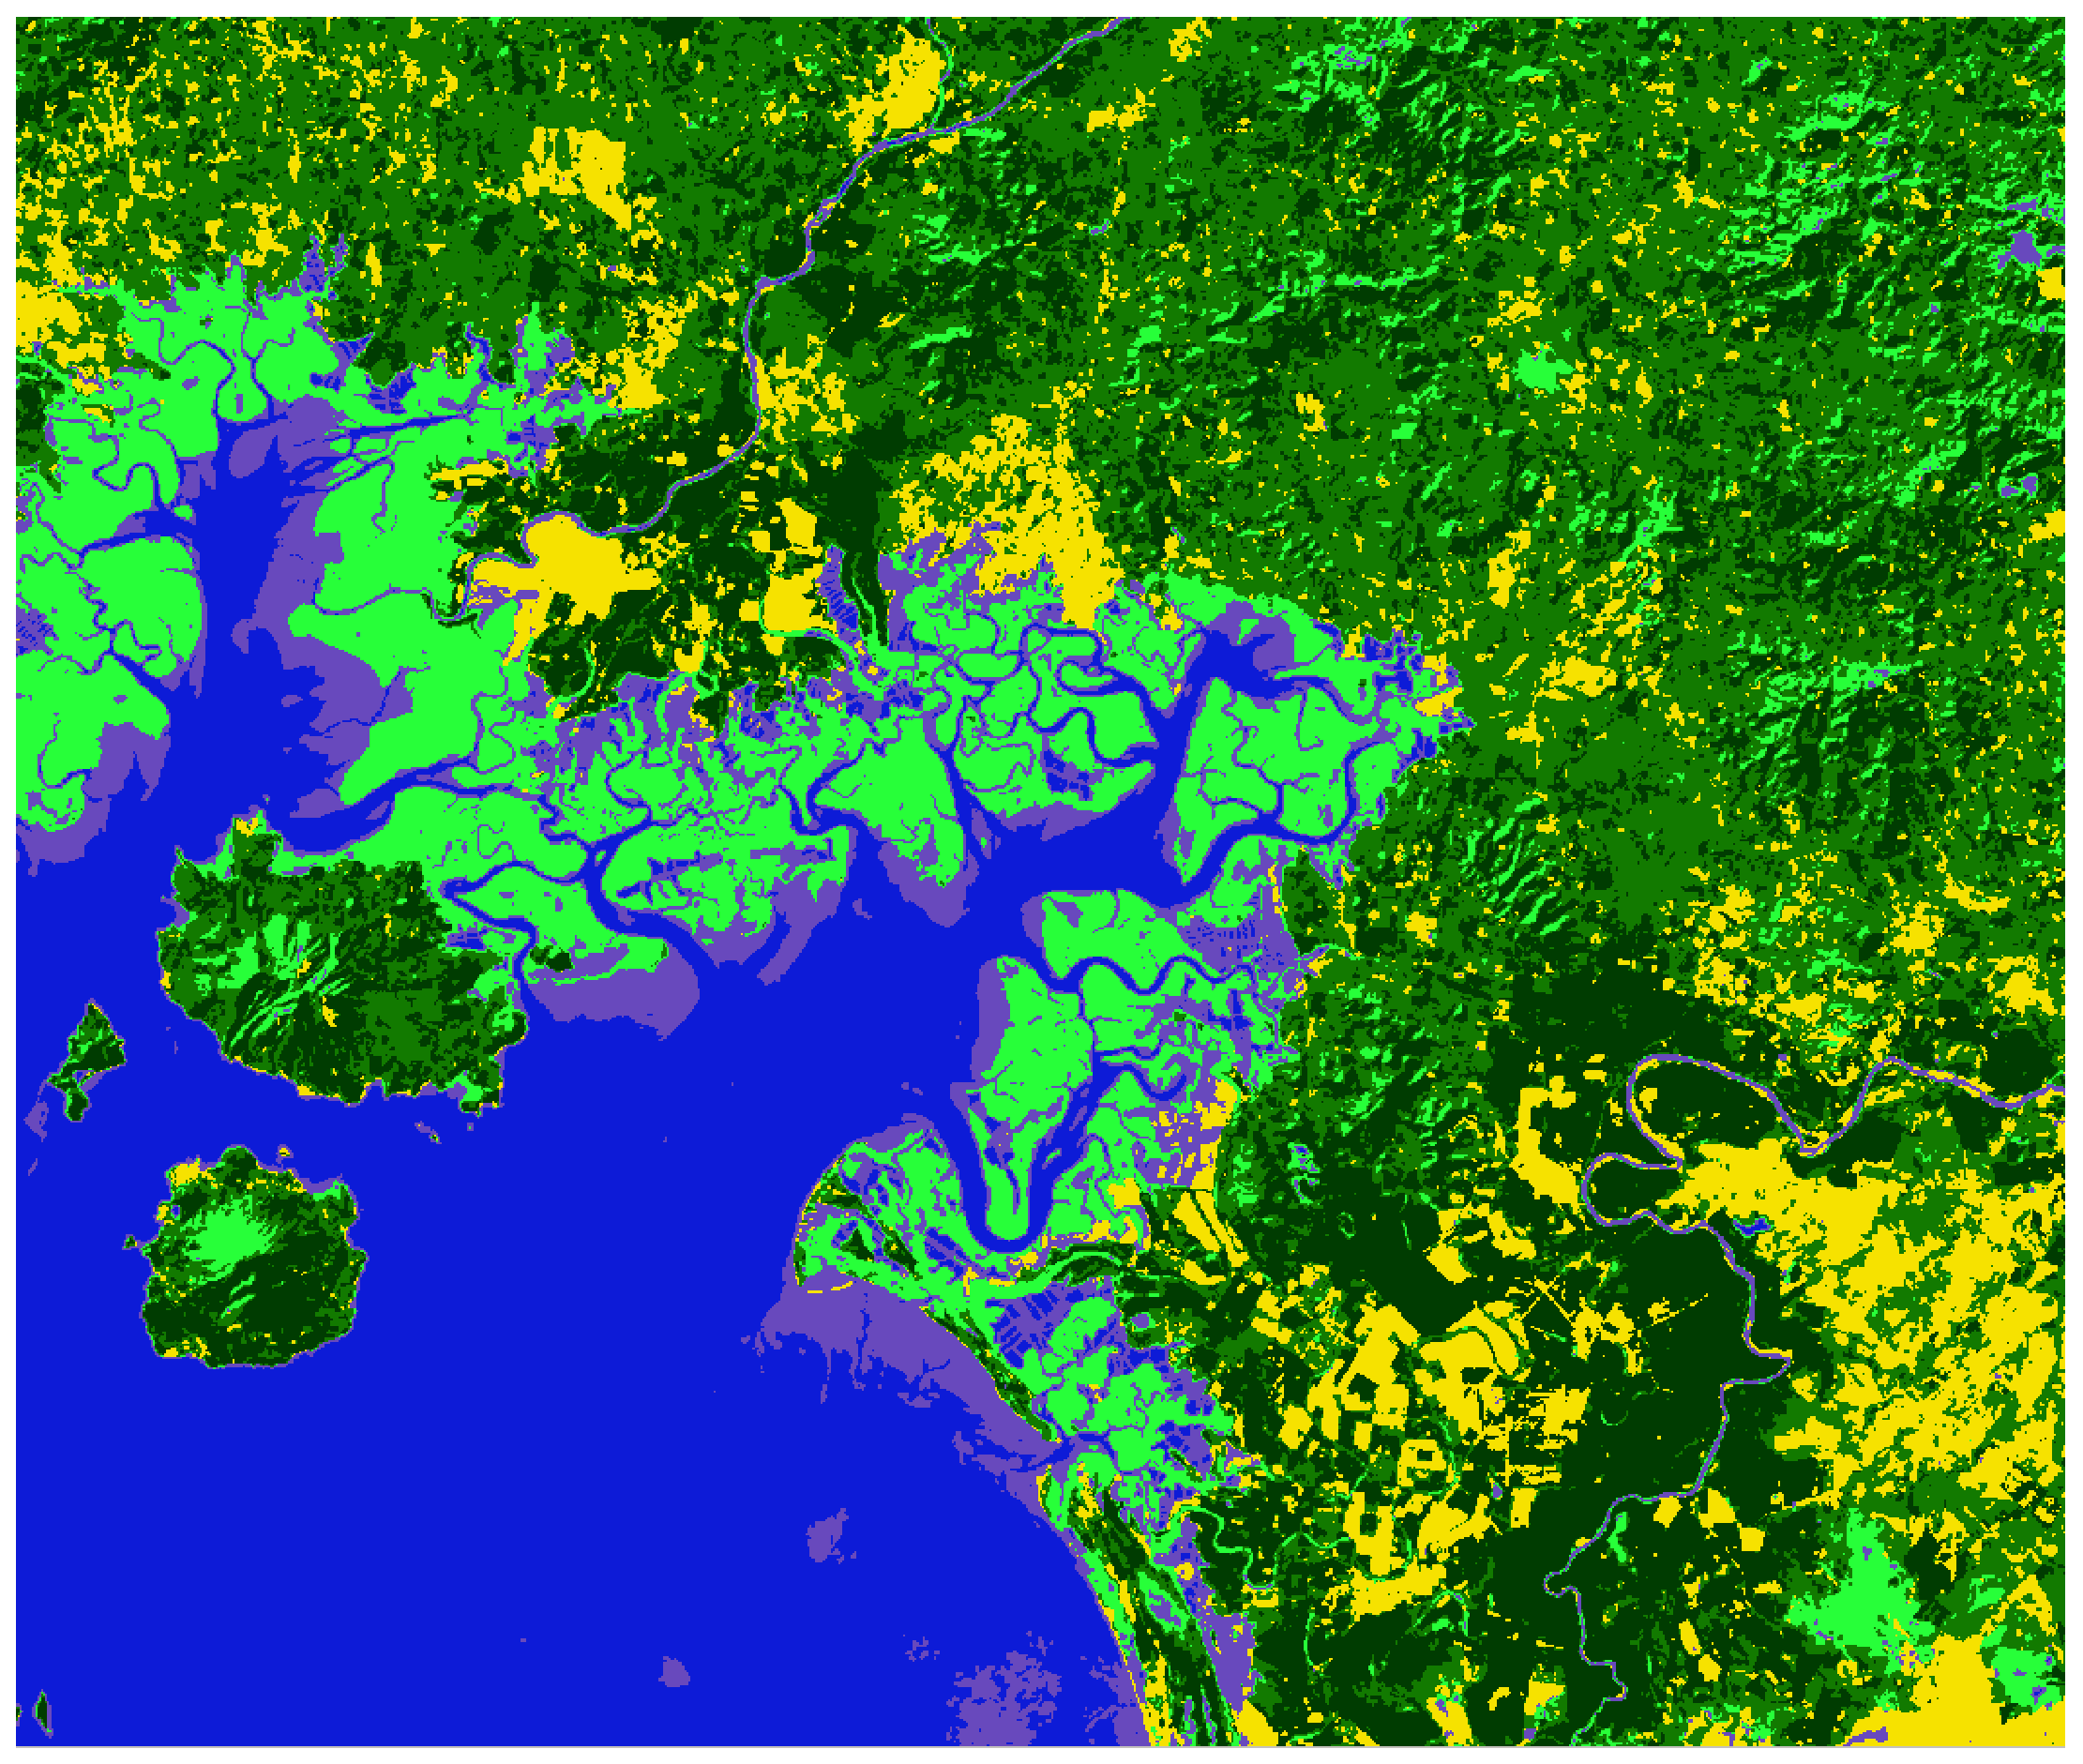
\includegraphics[width=0.8\linewidth]{./Imagenes/Detalle_clasnosup.eps}
	\captionsetup{font={footnotesize,it}}
	\caption[Detalle clasificación no supervisada]{Detalle de la clasificación no supervisada. Elaboración propia.}
	\label{fig:detalle_clasnosup}
\end{figure}

En cuanto a la clasificación utilizando el \ac{SAM} los resultados son buenos como se aprecia en el detalle de la figura \ref{fig:detalle_SAM}. Situándose el bosque de mangle en un intervalo de entre 0,35 y 0,67 rad (20,05º y 38,39º) se diferencia notablemente de otras cubiertas.

\begin{figure}
	\centering
	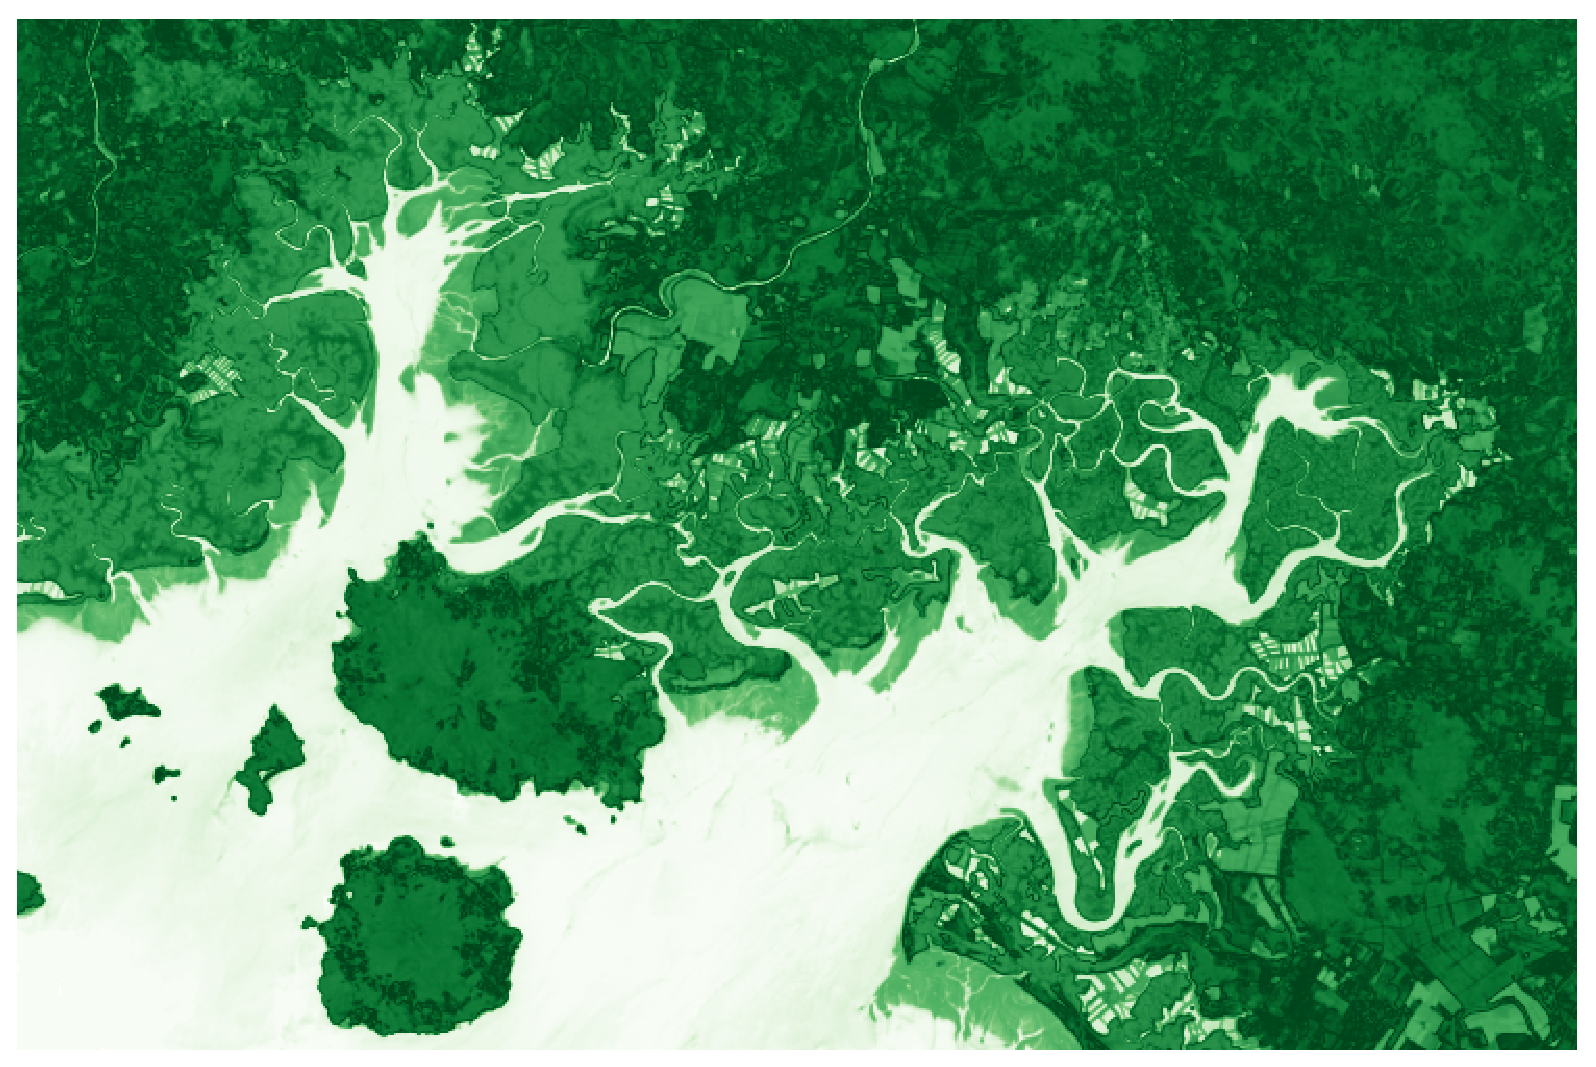
\includegraphics[width=0.8\linewidth]{./Imagenes/Detalle_SAM.eps}
	\captionsetup{font={footnotesize,it}}
	\caption[Detalle clasificación con \textit{Spectral Angle Mapper}]{Detalle de la clasificación con \ac{SAM}. Elaboración propia.}
	\label{fig:detalle_SAM}
\end{figure}

Se muestra el resultado de las clasificaciones en el anejo de mapas de este documento\footnote{Para generar los mapas se recurrió al uso del plugin de GRASS para QGIS}.

\section{Índices de vegetación}
El \ac{NDVI} nos muestra más claramente zonas de marisma o aguas turbias poco profundas que se sitúan en la línea de costa (figura \ref{fig:detalle_aguas}), justo donde hay presencia de bosque de mangle.%\Sep

\begin{figure}
	\centering
	\includegraphics[width=0.8\linewidth]{./Imagenes/Detalle_aguas.eps}
	\captionsetup{font={footnotesize,it}}
	\caption[Detalle marismas en NDVI]{Detalle de NDVI donde se ven las zonas de marisma. Imagen exportada de GRASS. Elaboración propia.}
	\label{fig:detalle_aguas}
\end{figure}

Gracias al índice \ac{SAVI} se pueden detectar fácilmente zonas de suelo desnudo y, sobre todo y más interesante, zonas de estanques artificiales, ya sean para cría de camarón, salineras o mixtas. En detalle se ven estas zonas en la figura \ref{fig:detalle_estanques} correspondientes a dos puntos distintos de la zona de estudio.%\Sep

\begin{figure}
	\centering
	\subfloat{
	\includegraphics[width=0.45\linewidth]{./Imagenes/Detalle_estanques.eps}}
	\subfloat{
	\includegraphics[width=0.45\linewidth]{./Imagenes/Detalle_estanques2.eps}}
	\captionsetup{font={footnotesize,it}}
	\caption[Detalle de estanques en SAVI]{Detalles de SAVI donde se ven los estanques artificiales. Imagenes exportadas de GRASSS. Elaboración propia.}
	\label{fig:detalle_estanques}
\end{figure}

Se muestra el resultado de los índices de vegetación en el anejo de mapas de este documento.

\section{Discusión}

La primera conclusión que se puede extraer de la realización de este \ac{TFG} es la referente a los datos tomados en campo. Podemos concluir que para la obtención de firmas para realizar bibliotecas espectrales tomar solamente una observación de cada especie se trate de una metodología correcta. Pero a la hora de realizar un análisis de separabilidad espectral fiable y, sobre todo, para hacer el posterior volcado de los resultados del análisis a la clasificación de imágenes satélite, resultaba óptimo tener numerosas observaciones de una misma especie. De este modo se permitiría conocer más a fondo aspectos de cada especie como desviación estándar de las observaciones con un valor central para cada banda que serían datos esenciales al hacer una clasificación supervisada de las imágenes Landsat.%\Sep

En cualquier caso, se preveía una dificultad el poder clasificar tres especies de mangle, que ya de por sí no están claramente separadas en el terreno, en una imagen de resolución espacial de 30 metros. Una posible solución a este problema sería el de tomar otro tipo de imagen satelital con mayor resolución espacial, como puede ser Spot o IKONOS, o realizar una fusión de imágenes combinando la mayor resolución espacial mencionada con la amplia resolución espectral de Landsat 8.%\Sep

Otro aspecto a tener en cuenta es el del software. Durante las distintas fases de realización del trabajo resultaron llamativas las numerosas actualizaciones que recibió el software. Y aunque la mayoría fueron actualizaciones menores que no afectaban a funciones importantes del programa, cabe destacar que el cambio de versión no resultó un problema de compatibilidad de archivos provenientes de versiones anteriores. En el caso de GRASS durante la realización del \ac{TFG} se liberó la versión estable 7.0 solo presentando problemas de traducción haciendo confuso el uso de algún comando o proceso, pero en ningún caso presentó problemas de compatibilidad entre versiones, salvo los evidentes a la hora de abrir un proyecto hecho en la versión anterior.%\Sep

Para la realización de la clasificación de las imágenes Landsat 8 se estudió la utilización de un plugin de QGIS llamado \ac{SCP} que permite hacer una clasificación supervisada y aplicar índices de vegetación de forma guiada por una interfaz de usuario perfectamente integrada en el software. Este plugin, creado por \cite{Congedo2015}, permite aplicar los clasificadores \ac{SAM}, el \ac{MLC} y \ac{NN} además de ofrecer una alternativa para obtener imágenes Landsat a las ya mencionadas en capítulos anteriores. Con el \ac{SCP} podemos importar archivos de firmas espectrales de forma sencilla.%\Sep

Una posible forma de mejorar la clasificación sería la de crear una máscara para la zona de más interés centrando esta en la costa del Golfo adentrándose unos kilómetros al interior. Un modo de realizar y aplicar esta máscara sería gracias al comando \textit{r.mask} de GRASS donde la podremos crear a partir de una capa ráster o vectorial que tengamos digitalizada en el proyecto y aplicarla dentro de las opciones del comando de clasificación. Otro aspecto a tener en cuenta para mejorar el resultado es la de ser más exhaustivos en la creación de las áreas de entrenamiento. En este caso se consideró suficiente el aproximarse a una media de 4000 píxeles por clase para obtener un resultado aceptable y verosímil, pero un incremento del número de píxeles en algunas clases ayudaría a definir mejor la clasificación e incluso, de tener un mayor conocimiento de la zona, crear algunas nuevas clases. También se podría haber hecho un análisis de \ac{CP} de la imagen.%\Sep

Cabe destacar también en cuanto a GRASS la utilidad de la herramienta \textit{Map Swipe} (\textit{g.gui.mapswipe}) que permite una mejor comparación de dos mapas superpuestos creando una ``cortinilla'' como se muestra en la figura \ref{fig:map_swipe}. Esta herramienta se implementó en la versión 7.0.

\begin{figure}
	\centering
	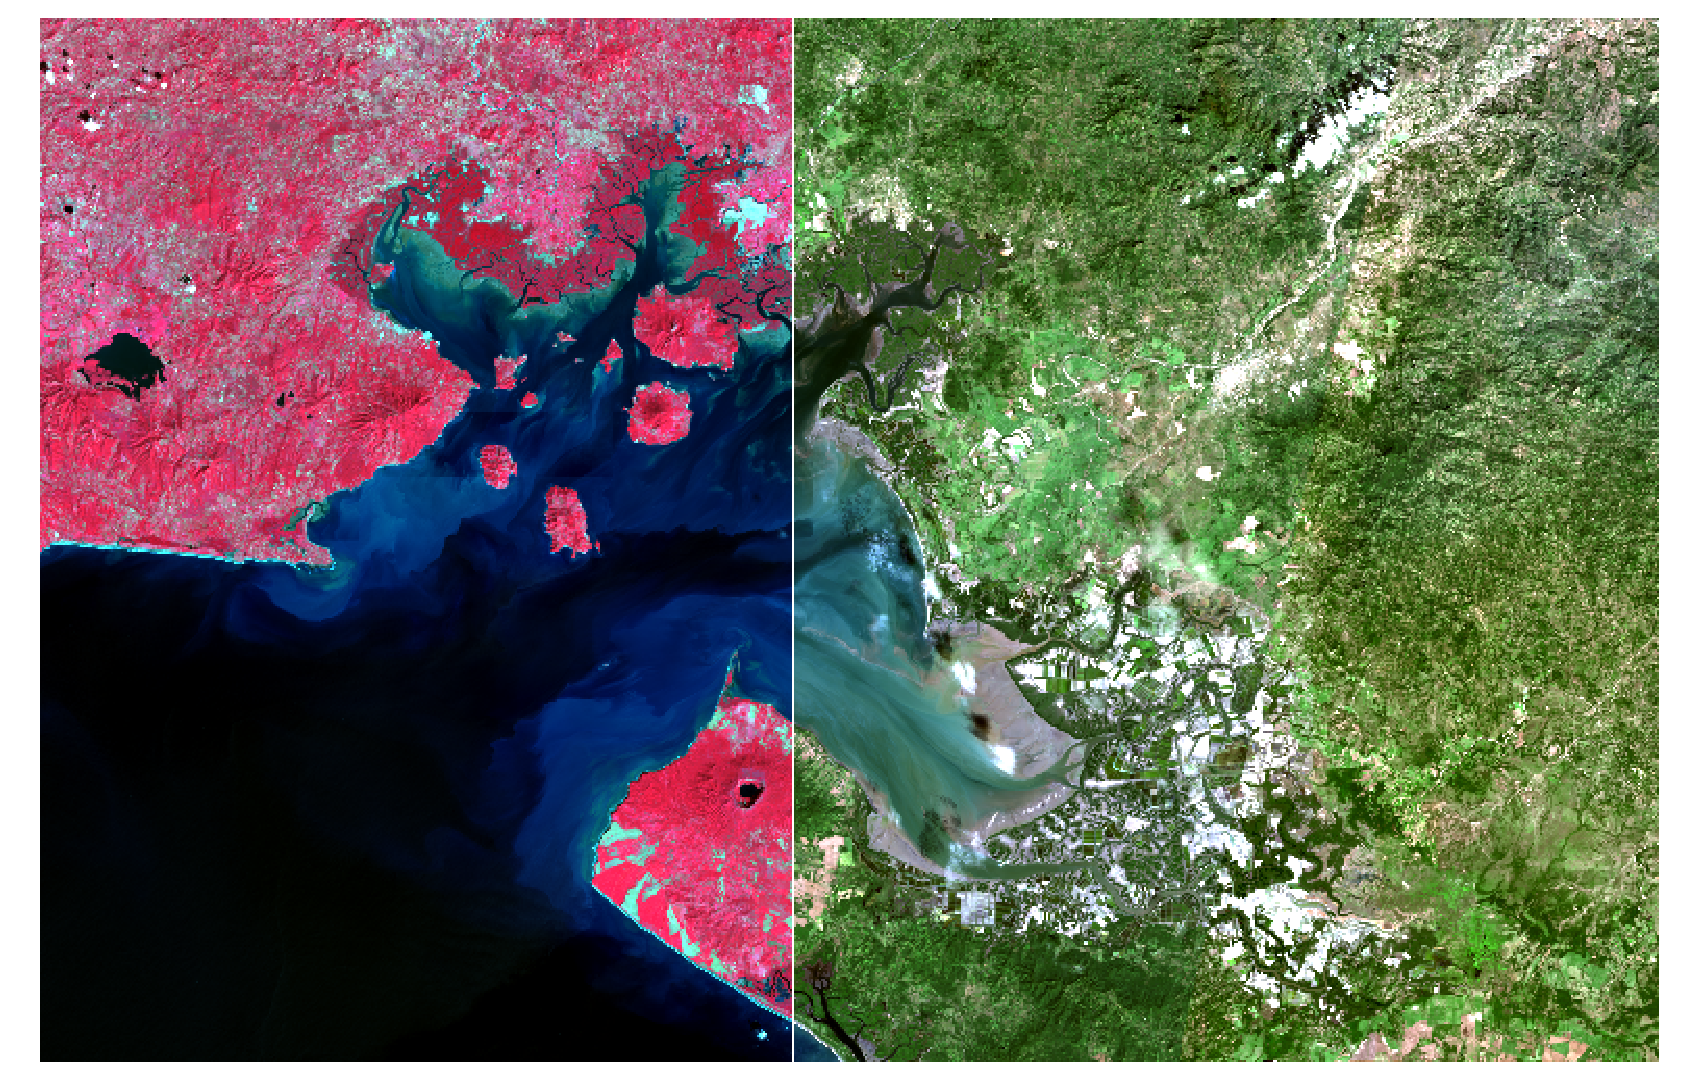
\includegraphics[width=0.9\linewidth]{./Imagenes/Map_swipe.eps}
	\captionsetup{font={footnotesize,it}}
	\caption[\textit{Map Swipe} de GRASS 7]{Ejemplo de \textit{Map Swipe} de GRASS 7. Se comparan combinaciones en falso color 5-4-3 y color real 4-3-2. Elaboración propia.}
	\label{fig:map_swipe}
\end{figure}

%CAPÍTULO 4. CONCLUSIONES
%MARCOS RIAL DOCAMPO
%Parte del documento principal TFG

%%%%%%%%%%%%%%%%%%
%% CONCLUSIONES %%
%%%%%%%%%%%%%%%%%%


\chapter{Conclusiones}

La primera conclusión que se puede extraer de la realización de este \ac{TFG} es la referente a los datos tomados en campo. Podemos concluir que para la obtención de firmas para realizar bibliotecas espectrales tomar solamente una observación de cada especie se trate de una metodología correcta. Pero a la hora de realizar un análisis de separabilidad espectral fiable y, sobre todo, para hacer el posterior volcado de los resultados del análisis a la clasificación de imágenes satélite, resultaba óptimo tener numerosas observaciones de una misma especie. De este modo se permitiría conocer más a fondo aspectos de cada especie como desviación estándar de las observaciones con un valor central para cada banda que serían datos esenciales al hacer una clasificación supervisada de las imágenes Landsat.\Sep

En cualquier caso, se preveía una dificultad el poder clasificar tres especies de mangle, que ya de por sí no están claramente separadas en el terreno, en una imagen de resolución espacial de 30 metros. Una posible solución a este problema sería el de tomar otro tipo de imagen satelital con mayor resolución espacial, como puede ser Spot o IKONOS, o realizar una fusión de imágenes combinando la mayor resolución espacial mencionada con la amplia resolución espectral de Landsat 8.\Sep

Otro aspecto a tener en cuenta es el del software. Durante las distintas fases de realización del trabajo resultaron llamativas las numerosas actualizaciones que recibió el software. Y aunque la mayoría fueron actualizaciones menores que no afectaban a funciones importantes del programa, cabe destacar que el cambio de versión no resultó un problema de compatibilidad de archivos provenientes de versiones anteriores. La única excepción fue el caso de GRASS, que durante la realización del \ac{TFG} liberó la versión estable 7.0 solo presentando problemas de traducción haciendo confuso su uso en algunos casos y por eso se prescindió de dicha actualización.\Sep

Para la realización de la clasificación de las imágenes Landsat 8 se estudió un plugin de QGIS llamado \ac{SCP}. Este plugin, creado por \cite{Congedo2015}, permite hacer una clasificación supervisada de forma guiada por una interfaz de usuario perfectamente integrada en QGIS. Además de ofrecer una alternativa para obtener imágenes Landsat a las ya mencionadas en capítulos anteriores, con el \ac{SCP} podemos importar archivos de firmas espectrales.\Sep

%------------------------%
%- BIBLIOGRAFÍA Y ANEJO -%
%------------------------%

\backmatter

\bibliographystyle{authordate1}
\bibliography{bibliografia}
\addcontentsline{toc}{chapter}{Bibliografía}

%ANEJO MAPAS
\appendix

%%MARCOS RIAL DOCAMPO
%Parte del documento principal TFG

%%%%%%%%%%%%%%%%%
%% ANEJO MAPAS %%
%%%%%%%%%%%%%%%%%

\chapter{Anejo. Mapas}
\section{Mapa1}
%\includepdf[pages=inicio-fin]{ruta archivo}
%anejomapas2

\chapter{Anejo. Mapas}

\newpage
$\ $
\thispagestyle{empty}

\immediate\write18{pdflatex mapas}
\clearpage
{\setlength\paperwidth{420mm}
\setlength\paperheight{297mm}
\setlength\pdfpagewidth\paperwidth
\setlength\pdfpageheight\paperheight
\includepdf[scale=1,noautoscale, %
                pagecommand={%
                \thispagestyle{empty}}]{./Mapas/Mapas.pdf}}
\clearpage

\immediate\write18{pdflatex mapas}
\clearpage
{\setlength\paperwidth{420mm}
\setlength\paperheight{297mm}
\setlength\pdfpagewidth\paperwidth
\setlength\pdfpageheight\paperheight
\newpage
$\ $
\thispagestyle{empty}
\clearpage

\immediate\write18{pdflatex mapas}
\clearpage
{\setlength\paperwidth{420mm}
\setlength\paperheight{297mm}
\setlength\pdfpagewidth\paperwidth
\setlength\pdfpageheight\paperheight
\includepdf[pages=2-2,scale=1,noautoscale, %
                pagecommand={%
                \thispagestyle{empty}}]{./Mapas/Mapas.pdf}}
\clearpage

\immediate\write18{pdflatex mapas}
\clearpage
{\setlength\paperwidth{420mm}
\setlength\paperheight{297mm}
\setlength\pdfpagewidth\paperwidth
\setlength\pdfpageheight\paperheight
\newpage
$\ $
\thispagestyle{empty}
\clearpage

\immediate\write18{pdflatex mapas}
\clearpage
{\setlength\paperwidth{420mm}
\setlength\paperheight{297mm}
\setlength\pdfpagewidth\paperwidth
\setlength\pdfpageheight\paperheight
\includepdf[pages=3-3,scale=1,noautoscale, %
                pagecommand={%
                \thispagestyle{empty}}]{./Mapas/Mapas.pdf}}
\clearpage

\immediate\write18{pdflatex mapas}
\clearpage
{\setlength\paperwidth{420mm}
\setlength\paperheight{297mm}
\setlength\pdfpagewidth\paperwidth
\setlength\pdfpageheight\paperheight
\newpage
$\ $
\thispagestyle{empty}
\clearpage

\immediate\write18{pdflatex mapas}
\clearpage
{\setlength\paperwidth{420mm}
\setlength\paperheight{297mm}
\setlength\pdfpagewidth\paperwidth
\setlength\pdfpageheight\paperheight
\includepdf[pages=4-4,scale=1,noautoscale, %
                pagecommand={%
                \thispagestyle{empty}}]{./Mapas/Mapas.pdf}}
\clearpage

\immediate\write18{pdflatex mapas}
\clearpage
{\setlength\paperwidth{420mm}
\setlength\paperheight{297mm}
\setlength\pdfpagewidth\paperwidth
\setlength\pdfpageheight\paperheight
\newpage
$\ $
\thispagestyle{empty}
\clearpage

\immediate\write18{pdflatex mapas}
\clearpage
{\setlength\paperwidth{420mm}
\setlength\paperheight{297mm}
\setlength\pdfpagewidth\paperwidth
\setlength\pdfpageheight\paperheight
\includepdf[pages=5-5,scale=1,noautoscale, %
                pagecommand={%
                \thispagestyle{empty}}]{./Mapas/Mapas.pdf}}
\clearpage

\end{document}